%%%%%%%%%%%%%%%%%%%%%%%%%%%%%%%%%%%%%%%%%%%%%%%%%%%%%%%             
%%         Este template foi adaptado por:           %%
%%                 Oton Crispim Braga                %%
%%    Bacharel em Ciência da Computação - IFCE       %%  
%%  Mestrando em Ciência da Computação - UFERSA/UERN %%
%%                                                   %%
%%                                                   %%
%%                                                   %%
%%                                                   %%
%%  A maior parte deste template foi recuperada      %%
%%         do trabalho desenvolvido por:             %%
%%                                                   %%        
%%            Ednardo Moreira Rodrigues              %%
%%       (Doutor em Engenharia Elétrica - UFC)       %%
%%                      &                            %%
%%            Alan Batista de Oliveira               %%
%%           (Engenheiro Eletricista - UFC)          %%
%%                                                   %%
%% Revisão:                                          %%
%%                                                   %%
%% - Francisco Edvander Pires Santos;                %%
%% - Juliana Soares Lima;                            %%
%% - Izabel Lima dos Santos;                         %%
%% - Kalline Yasmin Soares Feitosa.                  %%
%% - Eliene Maria Vieira de Moura;                   %%
%%                                                   %%
%% Colaboradores                                     %%
%%                                                   %%
%% -Andrei Bosco Bezerra Torres                      %% 
%% (Professor - Sistemas e Mídias Digitais -         %%
%% Instituto Universidade Virtual - UFC)             %%
%% Tiago ALves Lima                                  %% 
%% (Aluno de Mestrado em Eng. Elétrica)              %%
%%                                                   %%
%% Grande parte do trabalho foi adaptado do template %%
%% da UECE elaborado por:                            %%
%% Thiago Nascimento  (UECE)                         %%
%% Project available on:                             %%
%% https://github.com/thiagodnf/uecetex2             %%
%%                                                   %%
%% "Dúvidas, esclarecimentos ou sugestões podem ser  %%
%% enviadas para o seguinte e-mail:                  %%
%%                                                   %%
%%             atendimentobch@ufc.br                 %%
%%                                                   %%
%% As últimas atualizações estão descritas no inicio %%
%% do arquivo "README.md".                           %%
%%                                                   %%
%%%%%%%%%%%%%%%%%%%%%%%%%%%%%%%%%%%%%%%%%%%%%%%%%%%%%%%

\documentclass[        
    a4paper,          % Tamanho da folha A4
    12pt,             % Tamanho da fonte 12pt
    chapter=TITLE,    % Todos os capitulos devem ter caixa alta
    section=Title,    % Todas as secoes devem ter caixa alta somente na primeira letra
    subsection=Title, % Todas as subsecoes devem ter caixa alta somente na primeira letra
    oneside,          % Usada para impressao em apenas uma face do papel
    english,          % Hifenizacoes em ingles
    spanish,          % Hifenizacoes em espanhol
    brazil,           % Ultimo idioma eh o idioma padrao do documento
    fleqn             % Comente esta linha se quiser centralizar as equacoes. Comente também a linha 65 abaixo
]{abntex2}

\input{lib/preambulo}

\setlength{\mathindent}{0pt} %Complementa o alinhamento de equações para totalmente a esquerda.

%%%%%%%%%%%%%%%%%%%%%%%%%%%%%%%%%%%%%%%%%%%%%%%%%%%%%
%%                     ATENCAO                     %%
%%%%%%%%%%%%%%%%%%%%%%%%%%%%%%%%%%%%%%%%%%%%%%%%%%%%%
%  Qual e o nivel do trabalho academico que voce esta 
% escrevendo? Retire o simbolo "%" apenas de um dos 
% quatro topicos abaixo refente ao nível do seu traba
% -lho.

% \trabalhoacademico{tccgraduacao}
%\trabalhoacademico{tccespecializacao}
\trabalhoacademico{dissertacao}
%\trabalhoacademico{tese}

%%%%%%%%%%%%%%%%%%%%%%%%%%%%%%%%%%%%%%%%%%%%%%%%%%%%%

% Define se o trabalho e uma qualificacao
% Coloque 'nao' para versao final do trabalho

\ehqualificacao{nao}

% Remove as bordas vermelhas e verdes do PDF gerado
% Coloque 'sim' pare remover

\removerbordasdohyperlink{sim} 

% Adiciona a cor Azul a todos os hyperlinks

\cordohyperlink{nao}

%%%%%%%%%%%%%%%%%%%%%%%%%%%%%%%%%%%%%%%%%%%%%%%%%%%%%
%%         Informacao sobre a instituicao          %%
%%%%%%%%%%%%%%%%%%%%%%%%%%%%%%%%%%%%%%%%%%%%%%%%%%%%%

\ies{Universidade Federal Rural do Semi-Árido}
\iesdois{Universidade Estadual do Rio Grande do Norte}
\iessigla{UFERSA}
\iessigladois{UERN}
\centro{Centro de Ciências e Tecnologia}
\departamento{Departamento de Computação}

%%%%%%%%%%%%%%%%%%%%%%%%%%%%%%%%%%%%%%%%%%%%%%%%%%%%%
%%        Informacao para TCC de Graduacao         %%
%%%%%%%%%%%%%%%%%%%%%%%%%%%%%%%%%%%%%%%%%%%%%%%%%%%%%

\graduacaoem{Engenharia Xxxxxxx}
\habilitacao{bacharel} % Ou licenciado(a)

% AVISO: Caso necessario alterar o texto de apresenta-
% cao da Especializacao, ir a pasta "lib", arquivo 
% "ufctex.sty" na linha 502.


%%%%%%%%%%%%%%%%%%%%%%%%%%%%%%%%%%%%%%%%%%%%%%%%%%%%%
%%     Informacao para TCC de Especializacao       %%
%%%%%%%%%%%%%%%%%%%%%%%%%%%%%%%%%%%%%%%%%%%%%%%%%%%%%

\especializacaoem{Yyyyyyyyy}

% AVISO: Caso necessario alterar o texto de apresenta-
% cao da Especializacao, ir a pasta "lib", arquivo 
% "ufctex.sty" na linha 507.

%%%%%%%%%%%%%%%%%%%%%%%%%%%%%%%%%%%%%%%%%%%%%%%%%%%%%
%%         Informacao para Dissertacao             %%
%%%%%%%%%%%%%%%%%%%%%%%%%%%%%%%%%%%%%%%%%%%%%%%%%%%%%

\programamestrado{Programa de Pós-Graduação em Ciência da Computação}
\nomedomestrado{Mestrado Acadêmico em Ciência da Computação} % opicional
\mestreem{Ciência da Computação} 
\areadeconcentracaomestrado{Engenharia de Software e Sistemas Operacionais} % opicional

% AVISO: Caso necessario alterar o texto de apresenta-
% cao da dissertacao, ir a pasta "lib", arquivo 
% "ufctex.sty" na linha 511.

%%%%%%%%%%%%%%%%%%%%%%%%%%%%%%%%%%%%%%%%%%%%%%%%%%%%%
%%               Informação para Tese              %%
%%%%%%%%%%%%%%%%%%%%%%%%%%%%%%%%%%%%%%%%%%%%%%%%%%%%%

\programadoutorado{Programa de Pós-Graduação em Xxxxxx}
\nomedodoutorado{Doutorado em Xxxxxxx}
\doutorem{Engenharia Xxxxxx}
\areadeconcentracaodoutorado{Xxxxxxx}

% AVISO: Caso necessario alterar o texto de apresenta-
% cao da tese, ir a pasta "lib", arquivo "ufctex.sty" 
% na linha 515.

%%%%%%%%%%%%%%%%%%%%%%%%%%%%%%%%%%%%%%%%%%%%%%%%%%%%%
%%      Informacoes relacionadas ao trabalho       %%
%%%%%%%%%%%%%%%%%%%%%%%%%%%%%%%%%%%%%%%%%%%%%%%%%%%%%

\autor{João Marinho Neto} 
\titulo{Análise Automatizada de Objetivos de Desenvolvimento Sustentável: Uma Abordagem Baseada em Processamento de Linguagem Natural e Modelos de Linguagem de Grande Porte}
\data{2025}
\local{Mossoró}

% Exemplo: \dataaprovacao{01 de Janeiro de 2012}
\dataaprovacao{}

%%%%%%%%%%%%%%%%%%%%%%%%%%%%%%%%%%%%%%%%%%%%%%%%%%%%%
%%           Informação sobre o Orientador         %%
%%%%%%%%%%%%%%%%%%%%%%%%%%%%%%%%%%%%%%%%%%%%%%%%%%%%%

\orientador{Prof. Dr. Francisco Milton Mendes Neto}
\orientadories{UFERSA}
\orientadorcentro{Centro de Ciências e Tecnologia (CCT)} % opicional
\orientadorfeminino{nao} % Coloque 'sim' se for do sexo feminino

%%%%%%%%%%%%%%%%%%%%%%%%%%%%%%%%%%%%%%%%%%%%%%%%%%%%%
%%          Informação sobre o Coorientador        %%
%%%%%%%%%%%%%%%%%%%%%%%%%%%%%%%%%%%%%%%%%%%%%%%%%%%%%

% Deixe o nome do coorientador em branco para remover do documento

\coorientador{}
\coorientadories{SIGLA}
\coorientadorcentro{Centro do Coorientador (SIGLA)} % opicional
\coorientadorfeminino{nao} % Coloque 'sim' se for do sexo feminino

%%%%%%%%%%%%%%%%%%%%%%%%%%%%%%%%%%%%%%%%%%%%%%%%%%%%%
%%              Informação sobre a banca           %%
%%%%%%%%%%%%%%%%%%%%%%%%%%%%%%%%%%%%%%%%%%%%%%%%%%%%%

% Atenção! Deixe em branco o nome do membro da banca para remover da folha de aprovacao

% Exemplo de uso:
% \membrodabancadois{Prof. Dr. Fulano de Tal}
% \membrodabancadoisies{Universidade Federal do Ceará - UFC}

\membrodabancadois{Prof. Dr. Alex Sandro Gomes}
\membrodabancadoiscentro{}
\membrodabancadoisies{UFPE}
\membrodabancatres{Prof. Dr. Bruno de Sousa Monteiro}
\membrodabancatrescentro{}
\membrodabancatresies{UFERSA}
\membrodabancaquatro{}
\membrodabancaquatrocentro{}
\membrodabancaquatroies{}
\membrodabancacinco{}
\membrodabancacincocentro{}
\membrodabancacincoies{}
\membrodabancaseis{}
\membrodabancaseiscentro{}
\membrodabancaseisies{}

\begin{document}	

	% Elementos pré-textuais
	\imprimircapa
	\imprimirfolhaderosto{}
% 	\imprimirfichacatalografica{1-pre-textuais/ficha-catalografica} %  gerada pela biblioteca 
	%\imprimirerrata{elementos-pre-textuais/errata}
	\imprimirfolhadeaprovacao 
	\imprimirresumo{1-pre-textuais/resumo}
	\imprimirabstract{1-pre-textuais/abstract}
	\renewcommand*\listfigurename{Lista de Figuras} %Se você comentar esta linha o título da lista fica: LISTA DE ILUSTRAÇÕES
	\imprimirlistadeilustracoes
	\imprimirlistadetabelas
	%\imprimirlistadequadros
	%\imprimirlistadealgoritmos
	%\imprimirlistadecodigosfonte
	\imprimirlistadeabreviaturasesiglas
	%\imprimirlistadesimbolos{1-pre-textuais/lista-de-simbolos} % Comentado: requer makeglossaries extra
	\imprimirsumario
	
	\setcounter{table}{0}% Deixe este comando antes da primeira tabela.
	
	%Elementos textuais
	\textual
	\chapter{Justificativa}
\label{cap:justificativa}

A pesquisa se justifica pela crescente digitalização das experiências humanas e a
interconexão cada vez maior entre o físico e o virtual, que demandam uma compreensão
aprofundada de como as pessoas percebem e interagem com os mais diversos ambientes e
contextos. Este trabalho se insere nesse cenário, buscando explorar como a tecnologia pode não
apenas mediar, mas também auxiliar na compreensão e no enriquecimento da relação entre
indivíduos, lugares e suas identidades. A seguir, detalham-se os pilares que sustentam a relevância e
a oportunidade desta pesquisa.

\section{Relevância dos Princípios ESG no Contexto Atual}
\label{sec:relevancia-esg}

Embora o foco principal desta pesquisa não seja a avaliação direta do desempenho \gls{ESG} de
organizações -- sigla que representa os pilares Ambiental (\textit{Environmental}), Social (\textit{Social}) e de
Governança (\textit{Governance}) e se refere às práticas voltadas à sustentabilidade ambiental,
responsabilidade social e à qualidade de sua administração e transparência -- a consideração desses
princípios é fundamental no desenvolvimento e na aplicação de tecnologias que interagem com a
sociedade e o ambiente. Ferramentas que promovem o entendimento da identidade local e a
valorização do patrimônio cultural, por exemplo, dialogam com as dimensões sociais e de
governança ao fomentar o bem-estar comunitário, o respeito à diversidade e o uso consciente dos
recursos.

\section{A Crescente Necessidade de Compreender a Percepção e Identidade de Lugar}
\label{sec:necessidade-percepcao}

A forma como indivíduos e comunidades percebem e se identificam com os lugares que
habitam ou visitam é fundamental para o seu bem-estar, coesão social e para a preservação do
patrimônio cultural e natural. Na era digital, ferramentas interativas, como aplicativos de navegação
e plataformas de experiência turística e urbana, desempenham um papel cada vez mais significativo
na mediação dessa relação. Compreender profundamente como essas tecnologias moldam a
percepção dos usuários sobre os espaços, e como contribuem para a formação ou o reforço de sua
identidade territorial, é crucial. Este entendimento permite o desenvolvimento de intervenções
digitais mais sensíveis e eficazes, capazes de promover um sentimento de pertencimento genuíno e
uma valorização mais profunda dos contextos locais, indo além da simples funcionalidade para
tocar em aspectos emocionais e identitários da experiência humana.

\section{O Potencial da Análise de Sentimento e da Design Science para Inovação e Impacto}
\label{sec:potencial-analise}

Para desvendar as percepções e os sentimentos subjetivos dos usuários em relação aos
lugares, a análise de sentimento -- compreendida como a área do Processamento de Linguagem
Natural (\gls{NLP}) que visa extrair e identificar os estados afetivos e as opiniões subjetivas presentes
em textos \cite{liu2023esg} -- emerge como uma ferramenta analítica de grande potencial para
capturar as percepções públicas e acadêmicas. Ao aplicar algoritmos capazes de interpretar opiniões
e emoções expressas em dados textuais gerados a partir da interação com ferramentas digitais, é
possível obter resultados sobre a experiência do usuário que dificilmente seriam capturados por
métodos tradicionais. A condução desta pesquisa e o desenvolvimento da solução tecnológica
associada serão pautados pela metodologia da Design Science \cite{wieringa2014}. Esta
abordagem é particularmente adequada por focar na criação e avaliação de artefatos que resolvem
problemas identificados no mundo real, ao mesmo tempo em que geram conhecimento científico. A
combinação da análise de sentimento com os preceitos da Design Science justifica-se pela
oportunidade de criar uma ferramenta inovadora e validada para melhor identificar a percepção e a
identidade de lugar, contribuindo tanto para o avanço tecnológico quanto para a promoção de
experiências mais ricas, humanizadas e potencialmente mais alinhadas com um desenvolvimento
local sustentável.

	\chapter{Introdução}
\label{cap:introducao}

Nesta seção, são apresentados o contexto da pesquisa, a motivação, a metodologia da
pesquisa e as discussões e soluções que fundamentam este trabalho.

\section{Contexto da Pesquisa}
\label{sec:contexto}

Nos últimos anos, a relevância dos fatores ambientais, sociais e de governança (\gls{ESG}) têm
crescido significativamente no contexto empresarial e financeiro. A sigla ESG, utilizada
oficialmente pela primeira vez em um relatório da ONU, intitulado ``Who Cares Wins'' em 2004
\cite{onu2004}, refere-se a critérios que medem a sustentabilidade e o impacto ético de um
investimento em uma empresa. Desde então, os Princípios para Investimentos Responsáveis
(\gls{PRI}) da ONU, estabelecidos em 2006 \cite{onu2006}, reforçaram a importância dos critérios
ESG como princípios financeiros, formando a base da estrutura ESG que conhecemos hoje.

A pandemia de COVID-19 intensificou a atenção global aos temas ESG, especialmente em
relação às mudanças climáticas, proteção ambiental e saúde pública. A importância dos
investimentos a longo prazo, que consideram os riscos e oportunidades associados aos critérios
ESG, tornou-se mais evidente durante este período. As avaliações de processos econômicos
corporativos com base em ESG passaram a fornecer uma visão mais ampla, abrangendo tanto
posições regionais quanto globais.

Diversos estudos têm explorado a relação entre os conceitos de ESG e os investidores,
utilizando dados específicos de países ou focando em mercados financeiros específicos. Por
exemplo, alguns trabalhos analisaram como os dados de linguagem natural relacionados a ESG
impactam os mercados financeiros, enquanto outros examinaram os relatórios de responsabilidade
social corporativa (\gls{CSR}) para entender as concepções ESG. No entanto, esses estudos
frequentemente utilizam dados limitados ou não abrangem uma análise ampla, deixando lacunas no
entendimento sobre a utilização dos critérios ESG.

Neste contexto, a análise de sentimentos aplicada a dados relacionados a ESG emerge como
uma ferramenta para capturar as percepções públicas e acadêmicas. A análise de sentimentos, uma
subárea do processamento de linguagem natural (\gls{NLP}), permite a identificação de opiniões e
emoções expressas em textos, como notícias e publicações acadêmicas. Esta pesquisa busca auxiliar
na solução de um problema prático do mundo real utilizando a metodologia denominada Design
Science \cite{wieringa2014} para sua condução. Para isto seguiu-se uma estrutura lógica para
resolução do problema.

\section{Motivação}
\label{sec:motivacao}

Plataformas de exploração urbana e turística estão redefinindo a maneira como as pessoas se
conectam com os lugares, seu patrimônio e as narrativas locais. Ao permitir que os usuários
expressem suas impressões e vivências, abre-se uma nova janela para compreender a percepção e a
construção da identidade territorial. Neste contexto, a análise de sentimento emerge como uma
abordagem central para decifrar as nuances dessas interações e entender profundamente o que os
usuários sentem.

A ferramenta foco deste estudo, ao ser utilizada para explorar roteiros culturais ou interagir
com narrativas urbanas, não apenas guia o usuário, mas também se torna um canal para capturar
suas ricas experiências subjetivas. A aplicação da análise de sentimento sobre esses registros
permite identificar padrões emocionais e avaliar como as características de um lugar e as narrativas
associadas a ele ressoam com o público. O desenvolvimento e aprimoramento de uma solução
tecnológica com este propósito seguem uma abordagem metodológica estruturada, como a Design
Science, que orienta a criação de artefatos para solucionar problemas práticos e investigar
fenômenos reais. Entender, por exemplo, como o fato de ter nascido e/ou crescido em determinada
comunidade influenciou características culturais, sociais e aptidões políticas de um indivíduo é
crucial para definição de políticas públicas voltadas para educação e cultura daquele lugar, visando
preservar heranças passadas ou mesmo melhorar aspectos negativos identificados.

A análise sistemática das percepções e dos sentimentos dos usuários, capturados e
interpretados através desta plataforma, pode oferecer contribuições valiosas. Essas contribuições
podem direcionar também o aprimoramento de experiências turísticas e culturais, tornando-as mais
envolventes e significativas. Podem também informar como as pessoas estão percebendo e
construindo sua identidade com os espaços mediados pela ferramenta, fornecendo subsídios para
que esta se torne ainda mais eficaz em promover uma relação positiva com o entorno. A
compreensão profunda das reações emocionais, obtida via análise de sentimento, possibilita o
desenvolvimento de intervenções e recomendações mais personalizadas e eficazes através de
ferramentas de software, fortalecendo a conexão emocional e o senso de identidade dos usuários
com os lugares que exploram. Portanto, esta pesquisa se dedica a investigar como a análise de
sentimento aplicada aos dados gerados no Gnomon, uma plataforma digital interativa de exploração
urbana e turística, pode revelar e medir a percepção e a identidade de lugar formadas pelos seus
usuários.

\section{Metodologia da Pesquisa}
\label{sec:metodologia-pesquisa}

Para este trabalho seguiu-se uma estrutura lógica para resolução do problema. A seguir, as
questões de pesquisas que orientam este trabalho.

\subsection{Questões de Pesquisa}
\label{subsec:questoes-pesquisa}

As questões de pesquisa deste estudo empregam a abordagem Design Science para ajudar na
identificação dos problemas. Uma investigação guiada pelo Design Science adota uma metodologia
baseada na resolução de problemas \cite{wieringa2009}.

Em um cenário onde a responsabilidade social e a sustentabilidade se tornam cada vez mais
cruciais para a reputação e o sucesso das organizações, utilizar a análise de sentimento para melhorar
o desempenho ESG de organizações públicas é uma abordagem válida. Primeiramente, a análise de
sentimento permite que tenhamos a percepção do público sobre suas práticas ESG. Isso possibilita
uma resposta rápida a críticas e preocupações, demonstrando transparência. Além disso, com a
análise de grandes volumes de dados provenientes de redes sociais, notícias e outras fontes, é
possível identificar tendências e potenciais problemas antes que se tornem crises de reputação,
essencial para a gestão proativa das práticas ESG. Entender o sentimento do público também ajuda as
organizações a adaptar suas estratégias de comunicação, tornando-as mais eficazes. Mensagens que
ressoam com os valores e preocupações da sociedade podem aumentar o engajamento e o apoio às
iniciativas ESG. Ademais, a análise de sentimento pode fornecer informações sobre áreas onde as
práticas ESG podem ser melhoradas, permitindo que as organizações implementem mudanças
direcionadas e monitorem o impacto dessas melhorias ao longo do tempo. Então a questão geral de
pesquisa a ser tratada neste trabalho compreende:

\begin{citacao}
Como melhor identificar a percepção das pessoas sobre as práticas ESG e sua identidade de lugar?
\end{citacao}

Do ponto de vista organizacional, essa questão de pesquisa pode ser decomposta em outras
questões elementares. Segundo a Design Science, esta questão geral de pesquisa pode ser
categorizada em Questões Conceituais (QC), Questões Técnicas (QT) e Questões Práticas (QP).
Dessa forma, a Questão de Pesquisa enunciada acima pode ser decomposta nas seguintes questões de
pesquisa apresentadas a seguir:

\begin{alineas}
    \item \textbf{QC 1}: O que são Indicadores ESG?
    \begin{alineas}
        \item \textit{Explicação}: Essa questão busca identificar quais aspectos do ESG são mais relevantes e como eles podem ser representados em dados textuais para a análise de sentimento.
        \item \textit{Motivação}: Compreender os indicadores ESG e como eles funcionam.
    \end{alineas}
    \item \textbf{QT 2}: Como por meio de algoritmos de análise de sentimento podemos avaliar aspectos de ESG?
    \begin{alineas}
        \item \textit{Explicação}: Esta questão examina quais algoritmos de processamento de linguagem natural são mais eficazes para a análise de ESG.
        \item \textit{Motivação}: Identificar os algoritmos mais adequados pode melhorar a precisão e a relevância dos resultados obtidos.
    \end{alineas}
    \item \textbf{QP 3}: Como esses resultados podem ser utilizados para melhorar as práticas de ESG?
    \begin{alineas}
        \item \textit{Explicação}: Investigar formas práticas de aplicação dos valores obtidos pela análise de sentimento para promover melhorias nas práticas de ESG.
        \item \textit{Derivadas}: Quais são os principais desafios na implementação de melhorias baseadas em análise de sentimento?
    \end{alineas}
\end{alineas}

Em Design Science, a estruturação do conjunto de problemas de pesquisa é realizada através
da decomposição de uma questão geral de pesquisa em questões conceituais, técnicas e práticas. A
construção do conjunto de soluções ocorre pela composição das soluções apresentadas para essas
questões.

\subsection{Métodos de Pesquisa}
\label{subsec:metodos-pesquisa}

Para alcançar os objetivos pretendidos a pesquisa seguiu um conjunto de fases de acordo com
o Design Science \cite{wieringa2014}. O espaço-problema define a questão geral de pesquisa (QGP)
que foi decomposta em questões conceituais (QC), técnicas (QT) e práticas (QP). O espaço-solução
define as contribuições, composta pelos artefatos que respondem o conjunto de questões, conforme
ilustrado na Figura \ref{fig:metodologia-pesquisa}.

\begin{figure}[h]
    \centering
    \caption{Metodologia de Pesquisa}
    \label{fig:metodologia-pesquisa}
    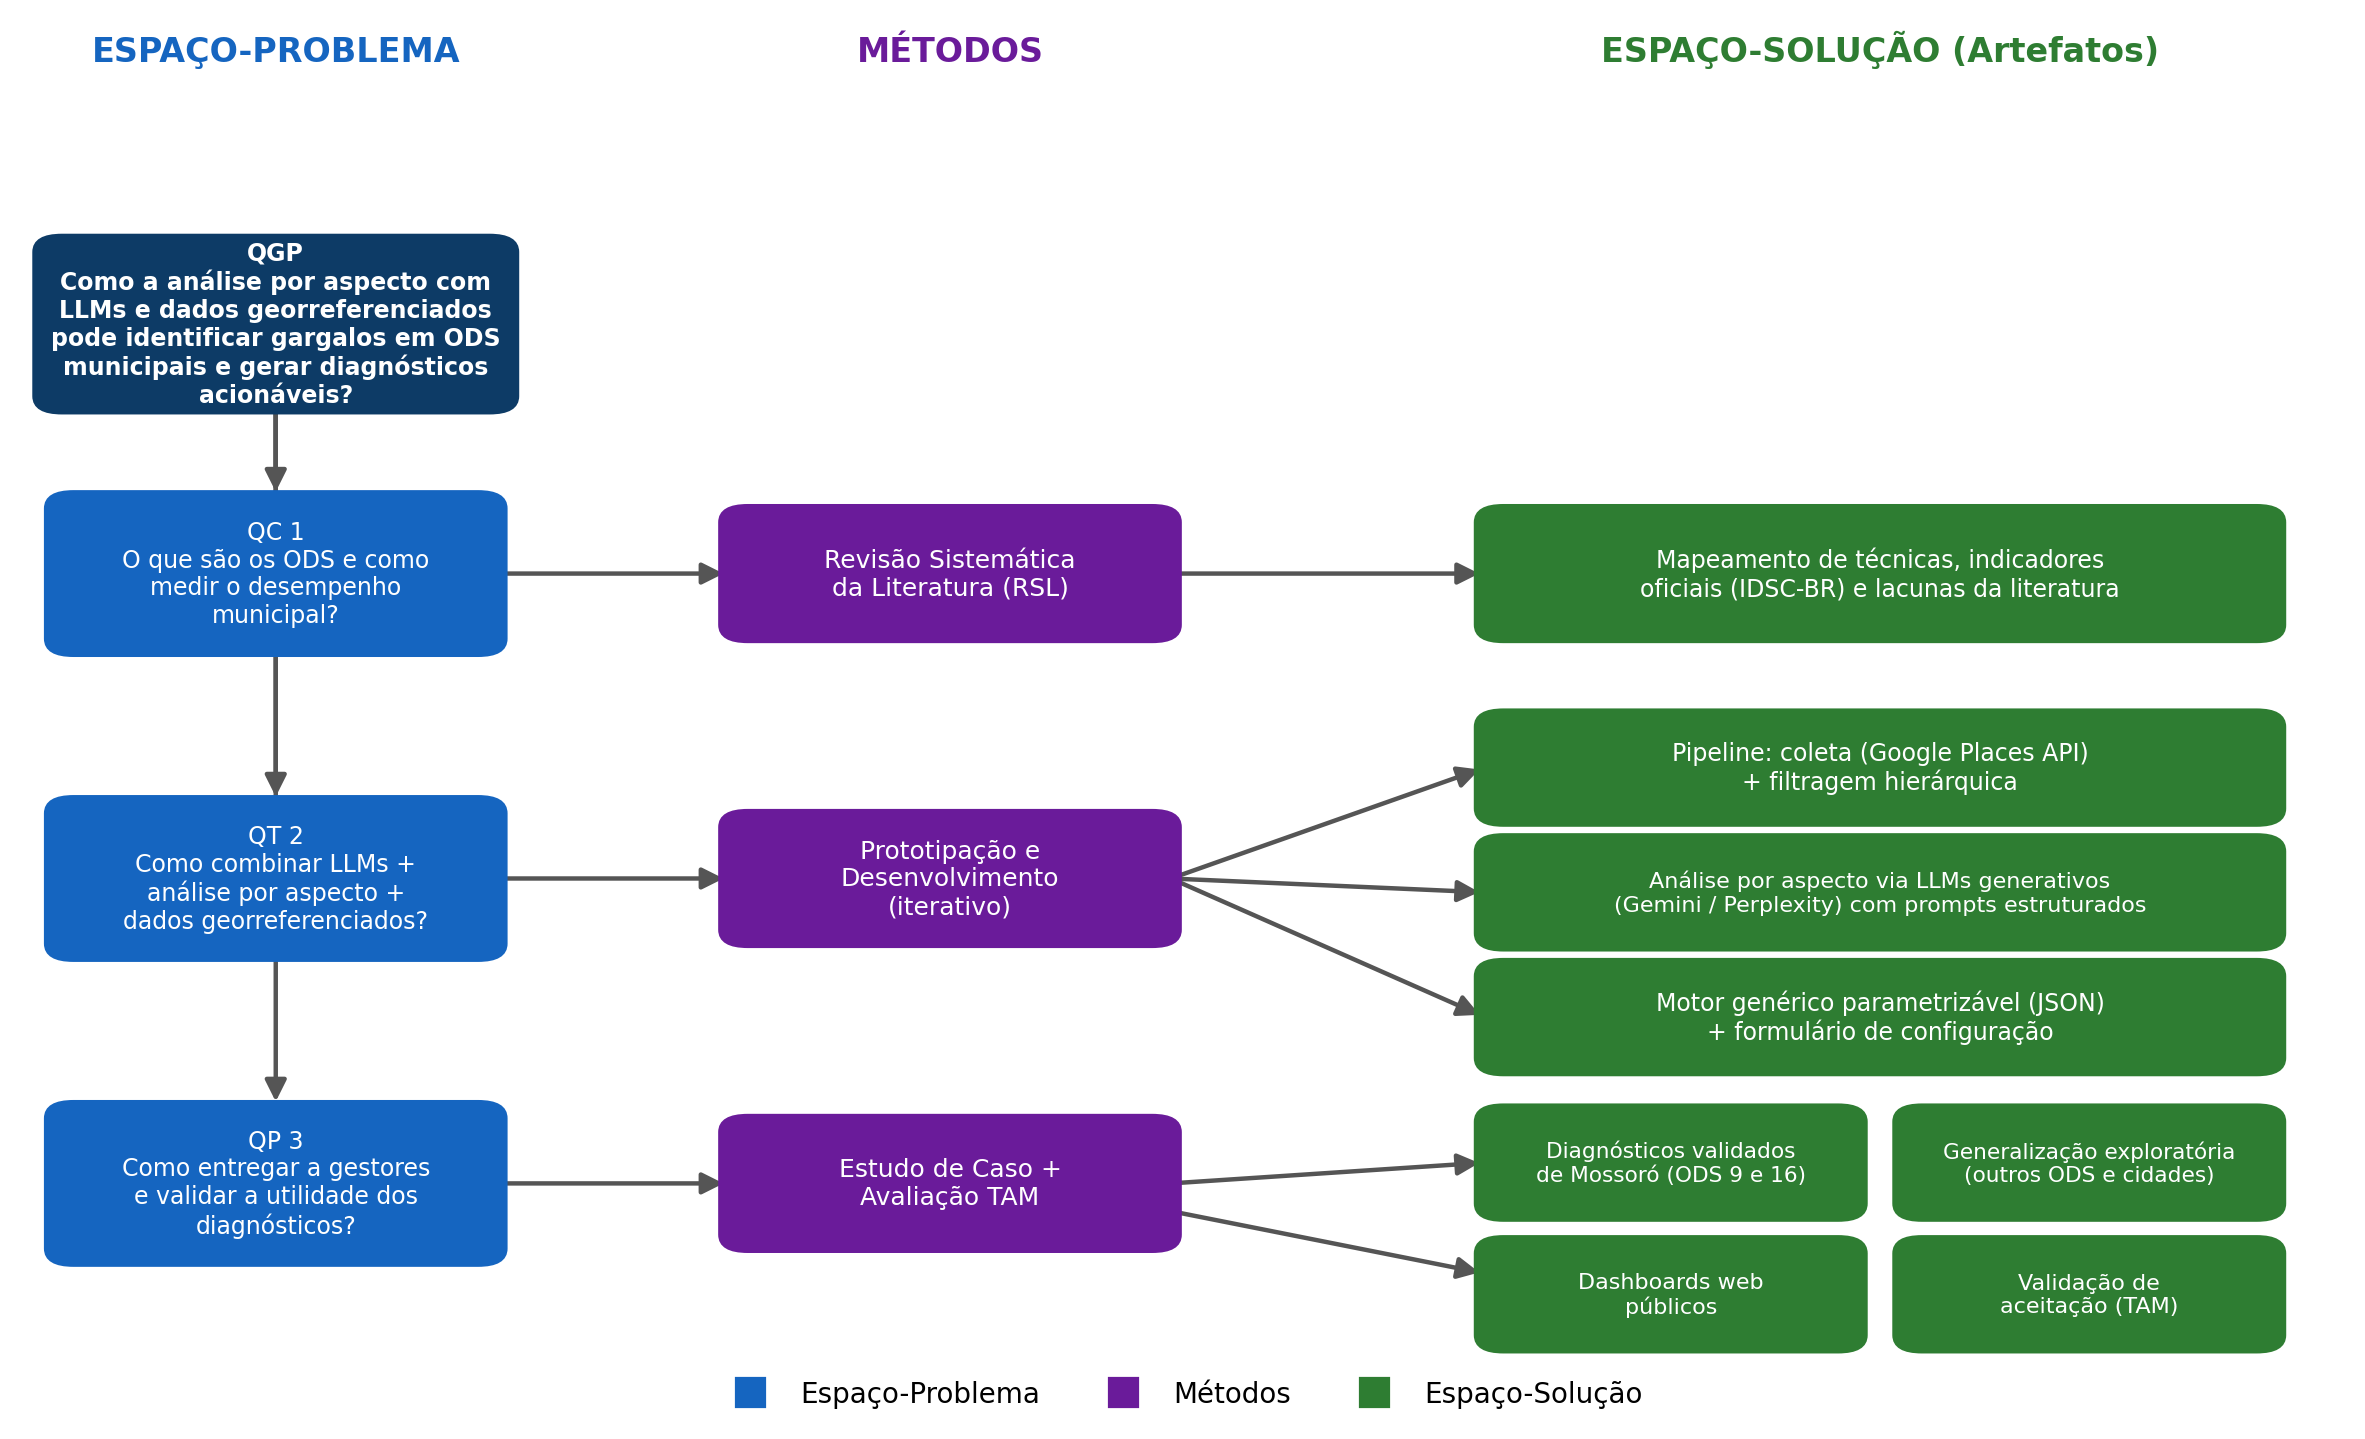
\includegraphics[width=0.85\textwidth]{figuras/metodologia-pesquisa}
    \legend{Fonte: Autoria Própria (2024).}
\end{figure}

Para responder às questões de pesquisa relacionadas ao uso de algoritmos de análise de
sentimento, com o intuito de melhorar o desempenho ESG (\textit{Environmental, Social, and Governance}),
serão adotados os seguintes métodos de pesquisa:

\begin{alineas}
    \item \textbf{Revisão Sistemática da Literatura (\gls{RSL})}: A RSL será utilizada para identificar e analisar estudos existentes sobre a aplicação de algoritmos de análise de sentimento em ESG. Este método permitirá uma compreensão abrangente dos principais indicadores ESG que podem ser extraídos de textos.
    \begin{alineas}
        \item \textit{Definição do Protocolo de RSL}: Estabelecer critérios de inclusão e exclusão, bases de dados a serem utilizadas e estratégias de busca.
        \item \textit{Coleta de Dados}: Realizar buscas em bases de dados acadêmicas como IEEE Xplore, ACM e Google Scholar.
        \item \textit{Análise e Sumarização}: Revisar e sintetizar os resultados dos estudos relevantes encontrados.
    \end{alineas}
    \item \textbf{Prototipação e Desenvolvimento}: A prototipação será utilizada para testar algoritmos de análise de sentimento adaptados ao contexto ESG. Este processo envolverá várias etapas de desenvolvimento, teste e refinamento.
    \begin{alineas}
        \item \textit{Seleção de Algoritmos}: Identificar algoritmos de NLP adequados, como modelos de Transformer (Modelo de rede Neural).
        \item \textit{Treinamento e Validação}: Treinar os algoritmos utilizando conjuntos de dados textuais relevantes (mídias sociais, relatórios financeiros, notícias) e validar sua eficácia com métricas como precisão, \textit{Recall} e F1-\textit{score}.
        \item \textit{Ajustes e Melhorias}: Refinar os algoritmos com base nos resultados.
    \end{alineas}
    \item \textbf{Estudo de Caso}: Aplicar os algoritmos desenvolvidos em um estudo de caso real para validar sua eficácia prática. Este estudo envolverá a utilização dos dados do Gnomon em situações reais.
    \begin{alineas}
        \item \textit{Seleção do Caso}: Definir um ou mais cenários de uso da ferramenta de exploração urbana e turística que permitam a coleta de dados relevantes para a análise de percepção e identidade de lugar.
        \item \textit{Coleta de Dados}: Obter dados gerados a partir da interação dos usuários com a ferramenta, como comentários, avaliações, e outros registros textuais que expressem suas percepções e sentimentos sobre os lugares explorados.
        \item \textit{Aplicação dos Algoritmos}: Aplicar os algoritmos de análise de sentimento para identificar e analisar as percepções dos usuários sobre os lugares e a formação de identidade de lugar, a partir dos dados coletados pela ferramenta.
        \item \textit{Avaliação dos Resultados}: Analisar os resultados gerados sobre a percepção e identidade de lugar, e avaliar a eficácia dos algoritmos e da ferramenta em capturar e interpretar esses aspectos, utilizando os resultados para refinar os algoritmos e métodos.
    \end{alineas}
\end{alineas}

\section{Discussões e Soluções}
\label{sec:discussoes-solucoes}

A revisão da literatura e a aplicação da ferramenta digital Gnomon em um estudo de caso
permitirão identificar aspectos da percepção de lugar e identidade territorial a partir de textos de
usuários, utilizando análise de sentimento. A eficácia de Modelos de Linguagem de Grande Porte
(\gls{LLM}s), como a \gls{API} Gemini, será avaliada para esta tarefa, com o suporte de estudos da
\gls{RSL} que demonstram o potencial de modelos NLP avançados como \gls{BERT} e \gls{RoBERTa}
para análises textuais detalhadas \cite{schimanski2024, gupta2024}.

A análise de sentimento buscará compreender profundamente como os usuários percebem os
lugares e expressam sua identidade ao usar o Gnomon. Esses resultados informarão o aprimoramento
da plataforma para enriquecer a experiência do usuário e sua conexão com o patrimônio e ambientes
explorados. No âmbito da Design Science, os resultados da análise de sentimento não apenas
responderão à questão de pesquisa sobre a identificação da percepção e identidade de lugar, mas
também oferecerão orientações práticas para o aprimoramento contínuo. O objetivo é fomentar o
desenvolvimento de experiências digitais mais significativas, personalizadas e que efetivamente
valorizem a relação humano-lugar.

	\chapter{Hipótese}
\label{cap:hipotese}

A aplicação de análise de sentimento automatizada, utilizando Modelos de Linguagem de
Grande Porte (\gls{LLM}s), como a \gls{API} Gemini, sobre dados textuais gerados por usuários na
plataforma digital Gnomon -- concebida e avaliada sob a metodologia da Design Science --
viabiliza uma identificação mais precisa e profunda da percepção dos usuários sobre os lugares e da
sua construção de identidade territorial. Adicionalmente, postula-se que esta mesma abordagem
analítica possui o potencial de revelar como dimensões de valor socioambiental, que podem se
alinhar a aspectos de Ambientais, Sociais e Governança (\gls{ESG}), são articuladas pelos usuários
em suas experiências e narrativas sobre esses territórios, conforme interagem com a plataforma
Gnomon. A investigação dessas capacidades permitirá o desenvolvimento e a validação de um
método robusto para compreender a experiência do usuário de forma integral, com implicações
diretas para o avanço do conhecimento sobre as intersecções entre tecnologia, identidade de lugar e
a expressão de valores contemporâneos.

Desta forma, a questão central que esta pesquisa busca responder por meio da validação
desta hipótese é:

\begin{citacao}
Como a análise de sentimento aplicada a dados da plataforma Gnomon pode melhor identificar a
percepção das pessoas sobre os lugares e sua identidade de lugar, e, secundariamente, capturar
suas considerações sobre aspectos socioambientais relacionados?
\end{citacao}

\chapter{Objetivo Geral}
\label{cap:objetivo-geral}

O objetivo geral desta pesquisa é investigar, propor e validar uma abordagem metodológica,
fundamentada na Design Science e na análise de sentimento com Modelos de Linguagem de
Grande Porte (LLMs), para identificar e compreender de forma aprimorada a percepção das pessoas
sobre os lugares e a formação de sua identidade de lugar, por meio da interação com a plataforma
digital Gnomon.

\section{Objetivos Específicos}
\label{sec:objetivos-especificos}

Para alcançar o objetivo geral, foram estabelecidos os seguintes objetivos específicos,
adaptados a partir dos focos de investigação de sentimento de pertencimento e percepção de temas
relevantes.

\subsection{Objetivos Específicos Relacionados ao Sentimento de Pertencimento}
\label{subsec:obj-pertencimento}

\begin{enumerate}
    \item \textbf{Identificar Expressões de Sentimento de Pertencimento nos Textos dos Usuários.}
    \begin{alineas}
        \item \textit{Descrição}: Mapear e catalogar palavras-chave, frases e construções linguísticas que indicam um sentimento de pertencimento nos relatos dos usuários.
    \end{alineas}

    \item \textbf{Analisar a Intensidade do Sentimento de Pertencimento.}
    \begin{alineas}
        \item \textit{Descrição}: Utilizar técnicas de análise de sentimentos para medir a intensidade (positiva, neutra, negativa) do sentimento de pertencimento expresso nos textos.
    \end{alineas}

    \item \textbf{Correlacionar o Sentimento de Pertencimento com Fatores Demográficos e Contextuais.}
    \begin{alineas}
        \item \textit{Descrição}: Investigar como variáveis como idade, gênero, origem geográfica influenciam o sentimento de pertencimento.
    \end{alineas}

    \item \textbf{Explorar a Evolução do Sentimento de Pertencimento ao Longo do Tempo.}
    \begin{alineas}
        \item \textit{Descrição}: Estudar como o sentimento de pertencimento dos usuários varia em períodos diferentes, identificando possíveis influências sazonais ou decorrentes de eventos específicos.
    \end{alineas}
\end{enumerate}

\subsection{Objetivos Específicos Relacionados à Percepção dos ODS da ONU}
\label{subsec:obj-ods}

\begin{enumerate}
    \item \textbf{Detectar Menções Diretas e Indiretas aos ODS nos Textos dos Usuários.}
    \begin{alineas}
        \item \textit{Descrição}: Aplicar técnicas de processamento de linguagem natural para identificar referências aos 17 \gls{ODS} nos relatos dos turistas, mesmo quando não mencionados explicitamente.
    \end{alineas}

    \item \textbf{Analisar o Sentimento Associado a Cada ODS Mencionado.}
    \begin{alineas}
        \item \textit{Descrição}: Avaliar a polaridade (positiva, neutra, negativa) das menções aos ODS, identificando quais objetivos são vistos de forma mais favorável ou enfrentam críticas.
    \end{alineas}

    \item \textbf{Avaliar o Nível de Conscientização e Conhecimento dos Indivíduos sobre os ODS.}
    \begin{alineas}
        \item \textit{Descrição}: Investigar o grau de familiaridade dos usuários com os ODS, considerando a profundidade das discussões e a precisão das informações apresentadas nos textos.
    \end{alineas}
\end{enumerate}

	\chapter{Revisão Sistemática da Literatura}
\label{cap:rsl}

Esta seção apresenta a Revisão Sistemática de Literatura, utilizada para selecionar trabalhos
relacionados com a proposta da pesquisa para mapear os que aplicam técnicas de análise de
sentimentos a dados ESG, com o objetivo de identificar as principais abordagens, desafios e
oportunidades.

A importância de uma \gls{RSL} reside em sua capacidade de fornecer uma visão abrangente e
metodologicamente rigorosa sobre um determinado campo de estudo. Seguindo uma metodologia
definida, este trabalho busca responder questões cruciais sobre as técnicas utilizadas na análise de
sentimentos aplicada a dados ESG. Ao fazer isso, espera-se contribuir para um entendimento mais
profundo e abrangente das melhores práticas e das lacunas de pesquisa existentes, promovendo o
avanço do conhecimento e a aplicação eficaz dos critérios ESG.

\section{Protocolo da RSL}
\label{sec:protocolo-rsl}

O objetivo de uma Revisão Sistemática da Literatura (RSL) é identificar, avaliar e discutir
trabalhos relevantes a fim de responder uma ou mais questões de pesquisa e identificar lacunas de
pesquisa. Esse objetivo deve ser alcançado através de uma metodologia bem definida, na qual
pode-se obter resultados menos enviesados \cite{dresch2015}.

\subsection{Metodologia da RSL}
\label{subsec:metodologia-rsl}

No protocolo da RSL, define-se, entre outras coisas, como será conduzida a execução da
revisão. O primeiro passo para a elaboração desse protocolo é a definição do objetivo da pesquisa.
O objetivo desta RSL é identificar abordagens para a análise de sentimentos aplicada a dados
relacionados aos princípios ESG utilizando técnicas de Processamento de Linguagem Natural (NLP).
Na Figura \ref{fig:metodologia-rsl} observa-se a metodologia adotada neste trabalho, baseada em
\citeauthor{dresch2015} \citeyear{dresch2015}.

\begin{figure}[h]
    \centering
    \caption{Metodologia da RSL}
    \label{fig:metodologia-rsl}
    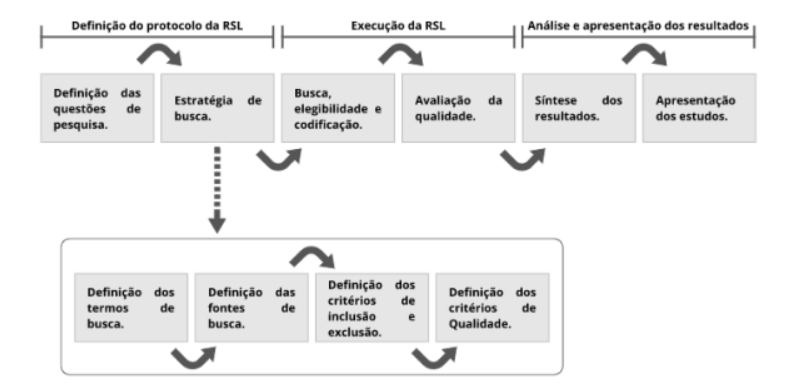
\includegraphics[width=0.85\textwidth]{figuras/metodologia-rsl}
    \legend{Fonte: \citeauthor{lopes2023} \citeyear{lopes2023}.}
\end{figure}

\subsection{Definição das Questões de Pesquisa}
\label{subsec:questoes-rsl}

Após estabelecer o objetivo, o passo seguinte na condução de uma revisão sistemática é
definir as questões de pesquisa que os estudos selecionados devem abordar. Esta etapa é crucial, pois
a habilidade de responder a essas questões é um dos principais critérios para a avaliação dos estudos
primários. Pode-se observar na Tabela \ref{tab:questoes-pesquisa} as questões de pesquisa definidas
para a RSL realizada neste trabalho.

\begin{table}[h]
\caption{Questões de Pesquisa}
\label{tab:questoes-pesquisa}
\begin{tabular}{p{1.5cm}p{11cm}}
\hline
\textbf{ID} & \textbf{Questões de Pesquisa (QP)} \\
\hline
QP1 & Quais técnicas de análise de sentimentos são utilizadas em dados relacionados a ESG? \\
QP2 & O que são indicadores ESG? \\
QP3 & Como a análise de sentimento pode ser utilizada para melhorar o desempenho ESG (\textit{Environmental, Social, and Governance}) de organizações públicas? \\
\hline
\end{tabular}
\legend{Fonte: Autoria Própria (2024).}
\end{table}

\subsection{Estratégia de Busca}
\label{subsec:estrategia-busca}

Após definir as questões de pesquisa, define-se a estratégia de busca dos estudos primários,
especifica-se os termos de busca, as fontes, os critérios de inclusão e exclusão e os critérios de
qualidade.

\subsection{Fontes de Busca}
\label{subsec:fontes-busca}

As fontes de buscas utilizadas para realizar a pesquisa foram:

\begin{alineas}
    \item IEEE Xplore
    \item Capes
    \item Science Direct
\end{alineas}

\subsection{Termos e String de Busca}
\label{subsec:termos-busca}

Para realizar a pesquisa nas fontes de busca selecionadas, os seguintes termos foram
escolhidos para compor a String de busca: ``ESG'', ``sentiment analysis'', ``public perception'' e
``NLP'' que foi inserida depois. Para abranger um maior número de artigos relacionados aos termos,
algumas variações foram adotadas, resultando na seguinte String de busca:

\begin{citacao}
(\textit{``ESG'' AND ``sentiment analysis'' AND ``public perception'' OR ``ESG'' AND ``NLP''}).
\end{citacao}

\subsection{Critérios de Inclusão e Exclusão}
\label{subsec:criterios}

Para filtrar os estudos primários foram definidos critérios de inclusão e exclusão que podem
ser conferidos nas Tabelas \ref{tab:criterios-inclusao} e \ref{tab:criterios-exclusao},
respectivamente.

\begin{table}[h]
\caption{Critérios de Inclusão}
\label{tab:criterios-inclusao}
\begin{tabular}{p{1.5cm}p{11cm}}
\hline
\textbf{ID} & \textbf{Critérios de Inclusão (CI)} \\
\hline
CI1 & Estudos publicados em periódicos (\textit{journals}) \\
CI2 & Estudos com texto completo acessível \\
CI3 & Estudos publicados entre 2020 e 2024 \\
CI4 & Estudos nos quais os termos de busca estejam presentes nos Metadados (título, resumo e palavras-chave) \\
\hline
\end{tabular}
\legend{Fonte: Autoria Própria (2024).}
\end{table}

\begin{table}[h]
\caption{Critérios de Exclusão}
\label{tab:criterios-exclusao}
\begin{tabular}{p{1.5cm}p{11cm}}
\hline
\textbf{ID} & \textbf{Critério de Exclusão (CE)} \\
\hline
CE1 & Estudos fora do objetivo da pesquisa e das questões de pesquisa. \\
\hline
\end{tabular}
\legend{Fonte: Autoria Própria (2024).}
\end{table}

\subsection{Critérios para Avaliação da Qualidade dos Estudos}
\label{subsec:criterios-qualidade}

Para avaliar a qualidade dos estudos incluídos nesta revisão sistemática, foram definidos três
critérios principais. O primeiro critério avalia a qualidade da execução do estudo, focando a precisão
e rigor metodológico. Os dois critérios seguintes avaliam, respectivamente, a adequação do estudo ao
objetivo da pesquisa e a pertinência do estudo ao contexto definido para esta RSL.

Cada estudo foi avaliado de acordo com esses três critérios, sendo classificados como de
qualidade alta, média ou baixa. A partir dessa avaliação, os estudos foram ranqueados globalmente,
seguindo a regra de que: um estudo será considerado de qualidade baixa se apresentar avaliação
baixa em qualquer um dos três critérios; será considerado de qualidade média se tiver pelo menos
um critério avaliado como médio e os demais como altos; e será considerado de qualidade alta se
todos os três critérios forem avaliados como altos. Estes critérios são apresentados na Tabela
\ref{tab:criterios-avaliacao}, adaptada de \citeauthor{lopes2023} \citeyear{lopes2023}.

\begin{table}[h]
\caption{Critérios de Avaliação}
\label{tab:criterios-avaliacao}
\begin{tabular}{p{2cm}p{4.5cm}p{4cm}p{4cm}}
\hline
\textbf{Critério} & \textbf{Qualidade da Condução do Estudo} & \textbf{Alinhamento com o Objetivo da Pesquisa} & \textbf{Relevância ao contexto de aplicação} \\
\hline
Alta & O estudo demonstra uma alta qualidade de execução, cumpre rigorosamente os padrões estabelecidos para o tema, segue o método proposto com precisão e apresenta resultados fundamentados em fatos e dados concretos. & O estudo trata diretamente do tema central da revisão sistemática. & O estudo foi conduzido em um contexto que corresponde exatamente ao definido para a revisão. \\
\hline
Média & O estudo apresenta uma qualidade de execução intermediária, com algumas lacunas em relação aos padrões exigidos para o tema, não segue completamente o método proposto e apresenta resultados que não são inteiramente baseados em fatos e dados. & O estudo aborda parcialmente o tema central da revisão sistemática. & O estudo foi realizado em um contexto que é semelhante ao definido para a revisão, mas com algumas diferenças. \\
\hline
Baixa & O estudo tem uma baixa qualidade de execução, não cumpre os padrões exigidos para o tema, não segue o método proposto e os resultados não são fundamentados em fatos e dados. & O estudo trata tangencialmente do tema central da revisão sistemática. & O estudo foi realizado em um contexto que difere significativamente do definido para a revisão. \\
\hline
\end{tabular}
\legend{Fonte: Adaptada de \citeauthor{lopes2023} \citeyear{lopes2023}.}
\end{table}

\section{Execução do Protocolo RSL}
\label{sec:execucao-rsl}

Após a definição do Protocolo de Revisão Sistemática da Literatura (RSL), inicia-se a fase de
sua implementação. Essa etapa envolve um processo meticuloso no qual os estudos primários são
identificados, selecionados e codificados. Primeiramente, realiza-se uma busca extensiva nas bases
de dados escolhidas, utilizando os termos e strings de busca previamente definidos. Os estudos
encontrados são então avaliados com base nos critérios de inclusão e exclusão estabelecidos no
protocolo.

\subsection{Busca, Elegibilidade e Codificação}
\label{subsec:busca-elegibilidade}

Durante a busca, tirou proveito dos recursos das ferramentas fornecidas pelas fontes de busca
para aplicar os critérios de inclusão e exclusão. As pesquisas nas respectivas fontes foram realizadas
no dia 06 de junho de 2024, totalizando em 73 artigos. Na plataforma IEEE Xplore retornou uma
quantidade baixa de trabalhos em relação ao Science Direct, que totalizaram 5 e 19, respectivamente.

Posteriormente, analisou-se os metadados (título, resumo e palavras-chave) de cada
trabalho, com o objetivo de desconsiderar aqueles que atendessem ao critério de exclusão que
resultou na exclusão de 51 trabalhos. Após a filtragem realizada por meio da leitura dos metadados,
restaram 8 potenciais estudos, os quais foram lidos por completo.

\subsection{Avaliação da Qualidade}
\label{subsec:avaliacao-qualidade}

Após a seleção dos trabalhos primários, seguiu-se para a avaliação de qualidade dos artigos,
que foi conduzida de acordo com os critérios de qualidade dos estudos descritos anteriormente. A
Tabela \ref{tab:avaliacao-qualidade} apresenta os resultados da avaliação da qualidade dos trabalhos
primários.

\begin{table}[h]
\caption{Avaliação de Qualidade}
\label{tab:avaliacao-qualidade}
\begin{tabular}{p{5cm}p{2.5cm}p{2cm}p{2cm}p{2.5cm}}
\hline
\textbf{Artigo} & \textbf{Autor} & \textbf{Qualidade da Execução} & \textbf{Adequação ao Objetivo} & \textbf{Adequação ao Contexto} \\
\hline
Um modelo de processamento de linguagem natural no BERT e técnica YAKE para extração de palavras-chave em Relatórios de Sustentabilidade & Gupta et al. (2024) & Alta & Alta & Média \\
\hline
Proposta de uma abordagem integrada para análise de dados ESG por meio de Algoritmos de Machine Learning e Deep Learning & Ook Lee et al. (2023) & Média & Média & Média \\
\hline
Percepções públicas sobre questões ambientais, sociais e de governança (ESG) baseadas sobre dados de mídia social: evidências da China & Liu et al. (2023) & Alta & Alta & Alta \\
\hline
Decodificando o humor do Twitterverse sobre investimentos ESG: mineração de opinião e temas principais usando aprendizado de máquina & Rachana Jaiswal et al. (2024) & Média & Alta & Média \\
\hline
Sentimento ESG baseado em notícias e risco de queda do preço das ações & Haixu Yu et al. (2023) & Alta & Alta & Alta \\
\hline
Reação dos Investidores às Notícias de ESG & Nyakurukwa et al. (2023) & Alta & Alta & Alta \\
\hline
O sentimento do mercado e as incertezas globais influenciam o nexo ESG-petróleo? Análise tempo-frequência & Purba et al. (2023) & Média & Média & Média \\
\hline
Preenchendo a lacuna na medição ESG -- Usando PNL para quantificar a Comunicação ESG & Schimanski et al. (2024) & Alta & Alta & Alta \\
\hline
\end{tabular}
\legend{Fonte: Autoria Própria (2024).}
\end{table}

\section{Análise e Apresentação dos Resultados}
\label{sec:analise-rsl}

Após a seleção e devida qualificação, os trabalhos passaram pela fase de análise dos dados
para que os artigos respondessem às questões de pesquisa apresentadas anteriormente. Na fase de
definição da estratégia de busca, o termo ``NLP'' foi incluído na string de busca mostrando que este
trabalho buscou por técnicas de processamento de linguagem natural.

Os estudos foram avaliados com base na qualidade da execução metodológica, adequação aos
objetivos da pesquisa e relevância do contexto de aplicação, permitindo uma compreensão
abrangente de suas contribuições e limitações. O estudo de \citeauthor{schimanski2024}
\citeyear{schimanski2024} destacou-se pela alta qualidade metodológica, utilizando modelos
avançados, como \gls{RoBERTa} e DistilRoBERTa, para analisar mais de 13,8 milhões de textos.
As precisões dos resultados demonstraram que técnicas de NLP podem quantificar comunicações de
ESG com confiabilidade, melhorando a transparência na avaliação da sustentabilidade corporativa.

\citeauthor{gupta2024} \citeyear{gupta2024} também apresentaram uma execução
metodológica de qualidade, alcançando 98\% de precisão na extração de palavras-chave de
relatórios de sustentabilidade utilizando a técnica YAKE e o modelo \gls{BERT}. Este estudo
confirmou a eficácia das técnicas de NLP na análise de grandes volumes de dados textuais,
proporcionando resultados detalhados.

O estudo intitulado ``Proposta de uma abordagem integrada para análise de dados ESG por
meio de Algoritmos de Machine Learning e Deep Learning'' mostrou uma qualidade metodológica
média. A pesquisa utilizou uma combinação de algoritmos de Machine Learning e Deep Learning
para analisar dados ESG, mas faltou rigor na validação dos modelos e consistência na aplicação das
técnicas. Apesar de promissora, a abordagem requer melhorias para garantir resultados mais
confiáveis.

\citeauthor{liu2023esg} \citeyear{liu2023esg} investigaram as percepções públicas sobre ESG
usando técnicas de análise de sentimentos em dados de mídia social. A metodologia foi bem
estruturada e os resultados validados, demonstrando que a análise de sentimentos pode capturar
percepções públicas, fornecendo visões sobre a opinião pública em relação a ESG. A análise do
humor no Twitter realizada pelo estudo ``Decodificando o Humor do Twitterverse'' apresentou uma
execução metodológica média. Utilizando aprendizado de máquina para analisar sentimentos na
plataforma, o estudo enfrentou limitações como a dependência de uma única fonte de dados.
Apesar disso, forneceu uma visão útil sobre as percepções de ESG no Twitter.

O estudo sobre o sentimento de notícias baseadas em ESG e seu impacto nos preços das
ações mostrou alta qualidade metodológica, utilizando boas técnicas de análise de sentimentos. Os
resultados indicaram que notícias de ESG influenciam significativamente o mercado financeiro,
demonstrando a importância de uma comunicação clara e transparente.

A pesquisa sobre a reação dos investidores às notícias de ESG também foi de alta qualidade,
utilizando técnicas avançadas de análise de sentimentos para entender as reações do mercado. Os
resultados validados rigorosamente indicaram que percepções de ESG têm um impacto direto no
comportamento dos investidores.

Por fim, o estudo sobre a influência do sentimento do mercado e incertezas globais no nexus
ESG-petróleo teve qualidade metodológica média. Embora relevante, apresentou limitações na
validação dos modelos e na abrangência metodológica, sugerindo a necessidade de maior rigor para
garantir a confiabilidade dos resultados.

Ao analisar cada estudo selecionado, para responder a primeira questão de pesquisa (QP1:
Quais técnicas de análise de sentimentos são utilizadas em dados relacionados a ESG?),
percebeu-se que os artigos revisados utilizaram várias técnicas avançadas de análise de sentimentos.
\citeauthor{schimanski2024} \citeyear{schimanski2024} aplicaram modelos de linguagem
pré-treinados como RoBERTa e DistilRoBERTa para analisar grandes volumes de textos.
\citeauthor{gupta2024} \citeyear{gupta2024} usaram a técnica YAKE junto com BERT para a
extração de palavras-chave de relatórios de sustentabilidade. Outros estudos, como o de
\citeauthor{liu2023esg} \citeyear{liu2023esg}, utilizaram aprendizado de máquina para analisar
dados de mídia social, enquanto pesquisas sobre reações de mercado a notícias de ESG empregaram
técnicas robustas de análise de sentimentos para avaliar o impacto das notícias no comportamento
dos investidores.

Dado os estudos selecionados com o objetivo de responder a segunda questão de pesquisa
(QP2: O que são indicadores ESG?) percebeu-se que indicadores ESG referem-se a métricas usadas
para avaliar o desempenho ambiental, social e de governança das empresas.
\citeauthor{schimanski2024} \citeyear{schimanski2024} e outros estudos revisados destacam que
esses indicadores são fundamentais para medir a sustentabilidade e a responsabilidade corporativa.
Eles abrangem uma ampla gama de fatores, incluindo emissões de carbono, práticas trabalhistas,
transparência corporativa e ética nos negócios.

Por fim, com o objetivo de responder a terceira questão de pesquisa (QP3: Como a análise de
sentimento pode ser utilizada para melhorar o desempenho ESG de organizações públicas?), a
análise de sentimentos pode fornecer visões sobre como as práticas de ESG são percebidas pelo
público e Stakeholders, ajudando a orientar melhorias. \citeauthor{liu2023esg}
\citeyear{liu2023esg} demonstraram que a análise de sentimentos de dados de mídia social pode
revelar percepções públicas sobre políticas ESG. Estudos como o de \citeauthor{gupta2024}
\citeyear{gupta2024} mostraram que a extração de palavras-chave de relatórios de sustentabilidade
pode identificar áreas de melhoria. Além disso, \citeauthor{schimanski2024}
\citeyear{schimanski2024} indicam que técnicas de NLP podem quantificar comunicações de ESG,
permitindo uma avaliação mais precisa e a identificação de tendências que podem informar decisões
estratégicas para melhorar o desempenho ESG.

	\chapter{Trabalhos Relacionados}
\label{cap:trabalhos-relacionados}

A literatura sobre análise automatizada de textos para diagnóstico de políticas públicas e avaliação de sustentabilidade tem crescido significativamente nos últimos anos, impulsionada pela disponibilidade de grandes volumes de dados não estruturados e pelo avanço dos Modelos de Linguagem de Grande Porte (\gls{LLM}s). Esta seção apresenta os principais trabalhos que contribuem para o embasamento teórico e metodológico desta dissertação, organizados em quatro eixos temáticos: análise de sentimentos aplicada a dados públicos, uso de \gls{NLP} para avaliação de políticas de sustentabilidade, aplicações de LLMs em contextos urbanos e o uso de dados do Google Places como fonte de diagnóstico.

\section{Análise de Sentimentos Aplicada a ESG e Políticas Públicas}
\label{sec:tr-esg}

\citeauthor{liu2023esg} \citeyear{liu2023esg} investigaram percepções públicas sobre fatores ambientais, sociais e de governança (\gls{ESG}) a partir de dados de mídia social coletados na China. O estudo utilizou técnicas de análise de sentimentos sobre textos de plataformas digitais e demonstrou que a opinião pública capturada de forma não estruturada pode antecipar e complementar indicadores ESG formais. A metodologia bem estruturada e os resultados validados demonstraram que a análise de sentimentos pode revelar percepções públicas que dificilmente seriam capturadas por métodos tradicionais de pesquisa. Este trabalho se relaciona diretamente com a presente dissertação ao validar o uso de dados textuais públicos para inferência sobre comportamentos coletivos ligados ao desenvolvimento sustentável.

\citeauthor{schimanski2024} \citeyear{schimanski2024} propuseram um framework para quantificar comunicações ESG utilizando \gls{NLP}. Os autores utilizaram modelos baseados em Transformers, como \gls{RoBERTa} e DistilRoBERTa, para analisar mais de 13,8 milhões de textos corporativos, demonstrando que técnicas de NLP podem medir com confiabilidade o nível de conformidade e transparência em reportes de sustentabilidade. A contribuição central deste trabalho é a evidência empírica de que modelos pré-treinados de linguagem podem ser adaptados para domínios altamente especializados, como a comunicação ESG, sem necessidade de \textit{fine-tuning} extensivo.

\citeauthor{jaiswal2024} \citeyear{jaiswal2024} analisaram o sentimento do mercado financeiro em relação a investimentos ESG por meio de mineração de opinião em dados do Twitter. O estudo revelou padrões temáticos e emocionais relevantes para a compreensão de como o público percebe iniciativas de sustentabilidade corporativa. Apesar de focar no contexto financeiro, o estudo contribui metodologicamente para a presente pesquisa ao demonstrar a viabilidade de análise de sentimentos em larga escala sobre textos curtos e heterogêneos.

\section{Uso de NLP para Avaliação de Sustentabilidade e ODS}
\label{sec:tr-ods-nlp}

\citeauthor{gupta2024} \citeyear{gupta2024} desenvolveram um modelo de processamento de linguagem natural baseado em \gls{BERT} combinado com a técnica YAKE para extração de palavras-chave em relatórios de sustentabilidade corporativa. O modelo alcançou 98\% de precisão na extração de termos relevantes, confirmando a eficácia de abordagens híbridas que combinam modelos neurais profundos com técnicas estatísticas de extração. O trabalho é relevante para a presente dissertação por demonstrar como modelos de NLP podem ser especializados para extrair informações estruturadas de textos sobre sustentabilidade.

\citeauthor{larosa2025} \citeyear{larosa2025} investigaram o potencial e as limitações dos LLMs na análise de políticas climáticas e de sustentabilidade. Os autores argumentam que LLMs genéricos oferecem vantagens significativas em contextos de baixa disponibilidade de dados rotulados, podendo realizar análise temática e identificação de lacunas em documentos de política pública sem necessidade de treinamento específico. Esta perspectiva é central para a justificativa metodológica da presente dissertação, que adota modelos de linguagem generativos (Gemini) para análise de textos públicos sobre ODS.

O trabalho de \citeauthor{abidoye2022} \citeyear{abidoye2022} discute a localização dos ODS por meio de dados desagregados, argumentando que indicadores nacionais ou estaduais frequentemente obscurecem disparidades locais críticas. Os autores defendem o investimento em coleta de dados granulares a nível municipal para avaliação mais precisa do progresso em direção às metas da Agenda 2030. Esta perspectiva reforça a relevância metodológica desta dissertação, que trata Mossoró-RN como unidade de análise e utiliza dados georreferenciados coletados no nível do estabelecimento.

\section{LLMs e Dados Urbanos para Diagnóstico de Políticas}
\label{sec:tr-llm-urbano}

\citeauthor{fu2023} \citeyear{fu2023} propuseram um framework de ciência urbana colaborativa baseado em LLMs pré-treinados, demonstrando que modelos como \gls{GPT} podem ser utilizados para análise de fenômenos urbanos complexos, incluindo mobilidade, habitação e uso do solo. O estudo demonstrou a viabilidade de integrar dados heterogêneos de fontes urbanas com análise gerada por IA, produzindo insights acionáveis para planejamento urbano. A abordagem proposta serve de referência para o uso de Gemini na presente dissertação para síntese e diagnóstico baseados em avaliações de usuários sobre estabelecimentos em Mossoró-RN.

\citeauthor{wankhade2022} \citeyear{wankhade2022} realizaram uma revisão abrangente de métodos de análise de sentimentos, aplicações e desafios. Os autores categorizaram as abordagens em três grupos: baseadas em léxico, baseadas em aprendizado de máquina tradicional e baseadas em aprendizado profundo. A revisão identificou que modelos baseados em Transformers (BERT, RoBERTa) representam o estado da arte em precisão, enquanto LLMs generativos emergem como alternativa flexível para contextos onde dados rotulados são escassos. Esta taxonomia orienta as escolhas metodológicas desta dissertação.

\citeauthor{agua2025} \citeyear{agua2025} investigaram o uso de LLMs para análise de sentimentos baseada em aspectos (\textit{aspect-based sentiment analysis}) em avaliações de clientes no setor de turismo. O estudo demonstrou que modelos de linguagem generativos podem identificar, sem treinamento adicional, sentimentos associados a aspectos específicos mencionados em textos livres -- exatamente a abordagem empregada nesta dissertação para classificar sentimentos relacionados às dimensões dos ODS 9 e ODS 16.

\section{Google Places como Fonte de Dados para Análise Urbana}
\label{sec:tr-google-places}

A utilização da Google Places API como fonte de dados para análise urbana e de políticas públicas é uma abordagem emergente que combina a ampla cobertura geográfica da plataforma com a riqueza qualitativa das avaliações de usuários. Diferentemente de pesquisas domiciliares ou questionários estruturados, as avaliações no Google Places refletem experiências espontâneas e não mediadas de cidadãos com estabelecimentos públicos e privados, tornando-as uma fonte valiosa para capturar percepções sobre qualidade de serviços, infraestrutura e segurança pública.

O IDSC -- Índice de Desenvolvimento Sustentável das Cidades \cite{idsc2024} -- calcula anualmente pontuações para os 17 ODS em municípios brasileiros a partir de indicadores primários como dados do IBGE, registros administrativos e pesquisas oficiais. Embora robusto para análises comparativas nacionais, o IDSC não fornece informações granulares sobre as causas específicas do baixo desempenho em determinado ODS. Esta dissertação propõe uma abordagem complementar ao IDSC, utilizando avaliações públicas do Google Places para diagnosticar, com especificidade local, os fatores que explicam as pontuações observadas.

Em síntese, os trabalhos revisados confirmam a viabilidade e relevância das escolhas metodológicas desta dissertação: a combinação de coleta automatizada de avaliações públicas, filtragem semântica multinível e análise por LLMs para diagnóstico de ODS é inovadora, replicável e alinhada com o estado da arte em análise de sentimentos, NLP para sustentabilidade e ciência urbana baseada em dados.

	\chapter{Materiais e Métodos}
\label{cap:materiais-metodos}

Nesta seção, detalha-se o enquadramento metodológico construído para
responder à questão central desta pesquisa: \emph{como a análise de
sentimento por aspecto, apoiada por Modelos de Linguagem de Grande Porte e
dados perceptivos georreferenciados, pode auxiliar a identificar gargalos
no desempenho de ODS municipais e gerar diagnósticos acionáveis para
políticas públicas?} Os conceitos teóricos que sustentam esta abordagem ---
incluindo a arquitetura Transformer, o modelo \gls{BERT}, os \gls{LLM}s
generativos e as técnicas de análise de sentimentos --- foram apresentados
no Capítulo~\ref{cap:fundamentacao-teorica}. Este capítulo concentra-se,
portanto, nas escolhas e procedimentos metodológicos, na seleção e
comparação das ferramentas de análise e nos resultados parciais obtidos
durante a fase de prototipação.

A modalidade metodológica adotada neste trabalho é a Design Science,
conforme definido por \citeauthor{wieringa2014} \citeyear{wieringa2014} e
detalhada no Capítulo~\ref{cap:introducao}. Esta escolha alinha-se aos
objetivos de desenvolver e avaliar um artefato tecnológico --- um sistema
automatizado de análise de ODS municipais --- e, simultaneamente, gerar
conhecimento sobre como técnicas de \gls{NLP} e \gls{LLM}s podem auxiliar
no diagnóstico de gargalos de desempenho em escala local. As etapas da
Design Science, envolvendo a construção do artefato, sua aplicação em
estudos de caso reais e a avaliação por especialistas, guiam a pesquisa. A
análise de sentimento por aspecto, aplicada a avaliações públicas
georreferenciadas coletadas via Google Places API, é o principal mecanismo
investigativo, permitindo a identificação sistemática de padrões e
problemas associados a estabelecimentos físicos concretos.

\section{Análise de Ferramentas}
\label{sec:analise-ferramentas}

A seleção de uma ferramenta ou abordagem para análise de sentimento
envolve considerar um espectro de opções, cada uma com suas características,
vantagens e desvantagens. Conforme detalhado no
Capítulo~\ref{cap:fundamentacao-teorica}, as abordagens disponíveis vão
desde métodos baseados em léxicos até modelos neurais profundos baseados em
Transformers e LLMs generativos.

Abordagens mais simples, como as baseadas em léxicos de polaridade e regras heurísticas --
a exemplo da biblioteca TextBlob, que oferece uma interface simplificada para tarefas de NLP,
incluindo análise de sentimento em Python \cite{loria2018}, e do modelo VADER (\textit{Valence Aware
Dictionary and sEntiment Reasoner}), especificamente desenvolvido e validado para a análise de
sentimento em textos de mídias sociais \cite{hutto2014} -- são fáceis de implementar e oferecem
resultados rápidos. O VADER, em particular, é otimizado para dados de mídias sociais. No entanto,
essas abordagens podem apresentar baixa precisão em textos com contextos complexos, ironia ou
gírias. Bibliotecas como NLTK também oferecem funcionalidades para análise de sentimentos,
muitas vezes combinando léxicos com aprendizado de máquina, mas podem requerer maior
configuração \cite{bird2009}.

O aprendizado de máquina tradicional, como o utilizado pelo FastText \cite{joulin2017},
que emprega \textit{word embeddings} e modelos lineares como a regressão logística para classificação de
texto, oferece maior eficiência e escalabilidade para grandes volumes de dados, mas geralmente
necessita de treinamento em volumes consideráveis de dados para alcançar bons resultados.

Modelos baseados em Transformers, como o BERT e suas variantes (RoBERTa, BERTimbau),
representam o estado da arte em termos de precisão para análise de sentimento contextual.
Plataformas como Hugging Face, através da biblioteca \textit{transformers} \cite{wolf2020}, facilitam o
acesso a esses modelos pré-treinados, que podem ser adaptados (\textit{fine-tuned}) para tarefas
específicas. Contudo, o \textit{fine-tuning} e a inferência com esses modelos podem ser
computacionalmente intensivos.

Paralelamente, existem serviços de NLP em nuvem, como o Google Cloud Natural Language
\gls{API} \cite{googlecloud2025} e o Azure Text Analytics, atualmente integrado ao Azure AI Language
\cite{microsoftazure2025}. Estes serviços oferecem APIs de fácil integração para análise de
sentimento e outras tarefas de NLP, sem a necessidade de gerenciamento de infraestrutura ou
treinamento de modelos por parte do usuário, embora geralmente impliquem custos e menor
controle sobre o modelo subjacente. Essas comparações podem ser vistas na Figura
\ref{tab:comparativa-ferramentas}.

\begin{figure}[h]
    \centering
    \caption{Tabela Comparativa das Ferramentas}
    \label{tab:comparativa-ferramentas}
    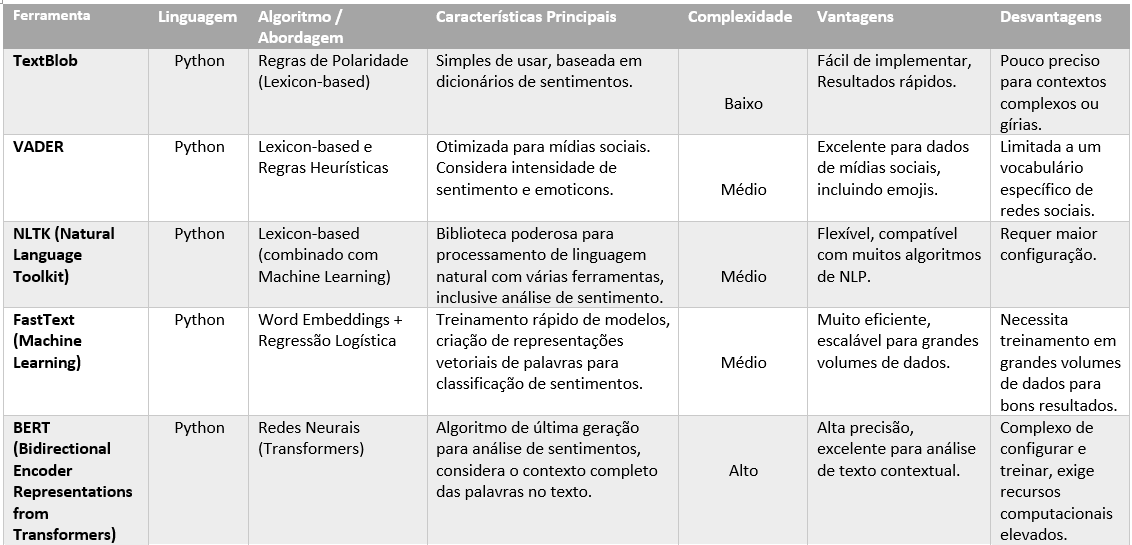
\includegraphics[width=\textwidth]{figuras/tabela-comparativa-ferramentas}
    \legend{Fonte: Autoria Própria (2025).}
\end{figure}

\section{Resultados Parciais}
\label{sec:resultados-parciais}

A análise das implementações desenvolvidas demonstrou que alguns modelos podem se sobressair a outros conforme veremos a seguir. Esta superioridade
manifesta-se através de diversas características técnicas que evidenciam tanto a eficiência quanto a
qualidade dos resultados obtidos.

A implementação com Gemini destaca-se inicialmente por sua simplicidade, como pode ser
visto na Figura \ref{fig:eficiencia-codigo}. Enquanto as implementações utilizando OpenAI e Cohere
requereram 146 linhas de código cada uma, a solução com Gemini é significativamente mais
concisa, utilizando apenas 89 linhas. Esta diferença não representa apenas uma economia de código,
mas reflete uma arquitetura mais elegante e menos propensa a falhas. Diferentemente das outras
APIs que necessitam de sistemas complexos de \textit{retry} -- ou seja, mecanismos que automaticamente
tentam enviar uma nova requisição em caso de falha -- para lidar com erros temporários, o Gemini
demonstrou maior estabilidade durante os testes, não apresentando falhas de processamento.

\begin{figure}[h]
    \centering
    \caption{Eficiência do Código}
    \label{fig:eficiencia-codigo}
    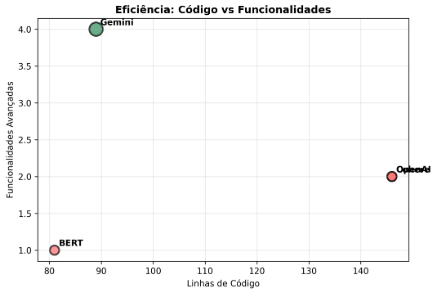
\includegraphics[width=0.85\textwidth]{figuras/eficiencia-codigo}
    \legend{Fonte: Autoria Própria (2025).}
\end{figure}

A capacidade de resposta estruturada do Gemini constitui outra vantagem significativa. O
modelo fornece não apenas a classificação do sentimento, mas também um valor de confiança
numérico e justificativas detalhadas para cada análise. Esta funcionalidade permite uma avaliação
mais precisa da qualidade dos resultados e facilita a interpretação dos dados por parte dos
pesquisadores. As justificativas geradas pelo Gemini demonstraram ser consistentemente mais
elaboradas e contextualmente relevantes conforme pode ser visto na Figura \ref{fig:nivel-confianca},
considerando tanto o conteúdo textual quanto as avaliações numéricas associadas aos \textit{reviews} de testes utilizados nas análises.

\begin{figure}[h]
    \centering
    \caption{Nível de Confiança}
    \label{fig:nivel-confianca}
    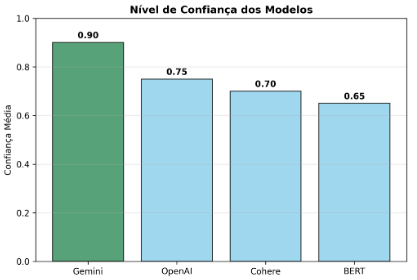
\includegraphics[width=0.85\textwidth]{figuras/nivel-confianca}
    \legend{Fonte: Autoria Própria (2025).}
\end{figure}

Em contraste, as limitações das outras implementações tornaram-se evidentes na comparação
conforme pode ser analisado na Figura \ref{fig:taxa-erro}. A solução OpenAI, embora robusta,
requer configurações mais verbosas com \textit{roles} de sistema, ou seja, instruções que definem como a
IA deve se comportar e responder, e demonstrou maior propensão a falhas temporárias durante os
testes. O sistema de \textit{retry} que foi preciso ser implementado, apesar de necessário para garantir
estabilidade, adiciona complexidade desnecessária ao código e pode impactar a velocidade de
processamento. Já a implementação com BERT multilingual, embora processe dados localmente, o
modelo que foi utilizado para teste apresentou limitações significativas como a restrição de 512
\textit{tokens} por texto e a dependência de classificações baseadas em estrelas, que se mostraram menos
interpretáveis para análises qualitativas.

\begin{figure}[h]
    \centering
    \caption{Taxa de Erro dos Modelos}
    \label{fig:taxa-erro}
    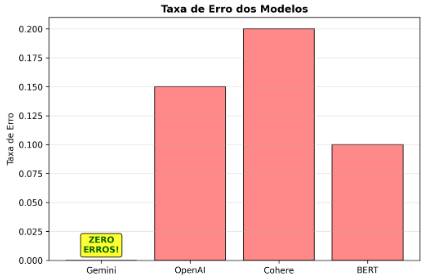
\includegraphics[width=0.85\textwidth]{figuras/taxa-erro}
    \legend{Fonte: Autoria Própria (2025).}
\end{figure}

Os resultados obtidos demostram uma possível superioridade do Gemini. A análise dos dados
processados revela que o modelo mantém uma confiança média consistente entre 0,8 e 0,95,
indicando alta precisão nas classificações. Mais importante ainda, durante todos os testes
executados, o Gemini não apresentou erros de processamento, demonstrando uma confiabilidade
operacional superior às demais soluções como pode ser visto na Figura \ref{fig:performance}. As
justificativas geradas pelo modelo mostram-se particularmente sofisticadas, considerando nuances
contextuais que outros modelos frequentemente ignoram.

\begin{figure}[h]
    \centering
    \caption{\textit{Performance}}
    \label{fig:performance}
    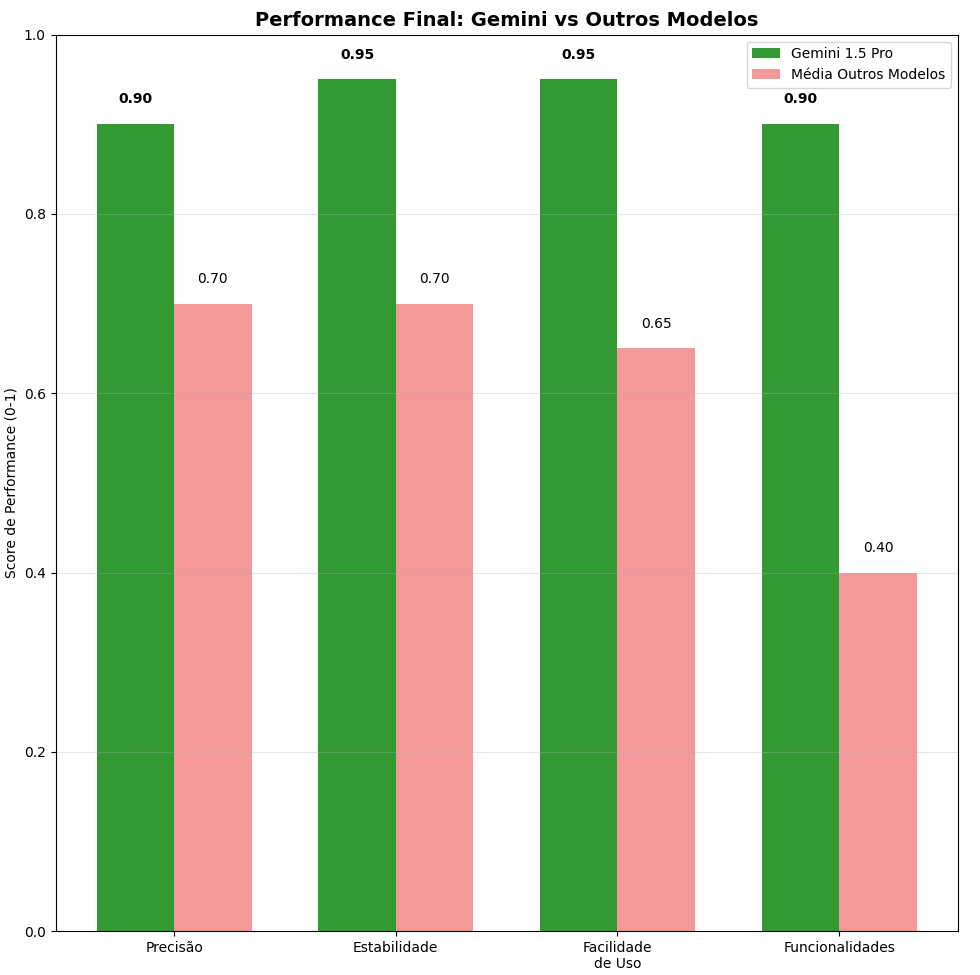
\includegraphics[width=0.85\textwidth]{figuras/performance}
    \legend{Fonte: Autoria Própria (2025).}
\end{figure}

Um exemplo representativo desta qualidade pode ser observado em uma análise onde o
Gemini identificou corretamente um sentimento positivo com confiança de 0,95, justificando que o
usuário descrevia o lugar como ótimo e sugeria atividades agradáveis para família e amigos,
reforçando esta interpretação com a avaliação numérica de 5 pontos. Esta capacidade de síntese
entre elementos textuais e numéricos demonstra uma compreensão contextual superior que se
traduz em resultados mais precisos e úteis para pesquisas acadêmicas.

Dessa forma, os resultados parciais estabelecem claramente que a implementação com
Google Gemini Pro constitui a solução mais promissora para análise de sentimentos em
\textit{reviews} com foco em sustentabilidade. A combinação de robustez técnica, capacidade analítica
superior, flexibilidade contextual e qualidade excepcional das respostas posiciona esta
implementação como ferramenta essencial para pesquisas em turismo sustentável e práticas ESG,
oferecendo não apenas maior precisão técnica, mas também funcionalidades avançadas que abrem
novas possibilidades de análise em estudos sobre percepções de sustentabilidade no setor turístico.

	\chapter{Implementação}
\label{cap:implementacao}

Este capítulo descreve em detalhe a implementação do sistema desenvolvido para análise automatizada de \glspl{ODS} a partir de avaliações associadas a locais físicos. O sistema foi construído em Python 3 e evoluiu de um protótipo específico para uma arquitetura generalizável, capaz de ser parametrizada para diferentes ODS, municípios e modelos de linguagem de grande porte. A implementação passou por três versões principais: a primeira voltada à análise ESG, a segunda composta por modelos específicos para o ODS 9 e o ODS 16, e a terceira consolidada como um motor genérico orientado por arquivos JSON de configuração.

\section{Arquitetura Geral do Sistema}
\label{sec:arq-geral}

O sistema é composto por quatro módulos principais:

\begin{enumerate}
    \item \textbf{Módulo de Configuração}: lê arquivos JSON que especificam o ODS alvo, município, termos de busca, aspectos a analisar, modelos de IA e parâmetros de execução;
    \item \textbf{Módulo de Coleta}: realiza buscas na Google Places API utilizando termos e coordenadas estratégicas do município, coletando avaliações (\textit{reviews}) dos estabelecimentos encontrados;
    \item \textbf{Módulo de Filtragem e Pré-processamento}: aplica filtros hierárquicos de validação geográfica, relevância por tipo de local e qualidade de conteúdo;
    \item \textbf{Módulo de Análise com IA}: envia cada comentário filtrado a uma LLM para classificação de sentimento por aspecto do ODS, geração de justificativas e extração de palavras-chave.
\end{enumerate}

\clearpage

A Figura~\ref{fig:fluxo-pipeline} sintetiza o fluxo operacional da solução, desde a configuração inicial do experimento até a disponibilização dos resultados em \textit{dashboards}.

\begin{figure}[!t]
    \centering
    \caption{Fluxograma da pipeline de análise automatizada de ODS}
    \label{fig:fluxo-pipeline}
    \normalsize
    \setlength{\fboxsep}{6pt}
    \renewcommand{\arraystretch}{1.0}
    \begin{tabular}{c}
        \fbox{\parbox{0.78\textwidth}{\centering \textbf{1. Configuração JSON}\\Definição do ODS, município, dimensões, termos de busca, bases de dados e modelos de IA}}\\[0.18cm]
        $\downarrow$\\[0.18cm]
        \fbox{\parbox{0.78\textwidth}{\centering \textbf{2. Busca no Google Places API}\\Consulta de locais físicos associados aos termos configurados e às coordenadas do município}}\\[0.18cm]
        $\downarrow$\\[0.18cm]
        \fbox{\parbox{0.78\textwidth}{\centering \textbf{3. Detalhes do Local}\\Coleta de nome, endereço, coordenadas, avaliação média e comentários públicos disponíveis}}\\[0.18cm]
        $\downarrow$\\[0.18cm]
        \fbox{\parbox{0.78\textwidth}{\centering \textbf{4. Filtros}\\Validação geográfica, deduplicação, comprimento mínimo, relevância semântica e adequação ao ODS}}\\[0.18cm]
        $\downarrow$\\[0.18cm]
        \fbox{\parbox{0.78\textwidth}{\centering \textbf{5. Análise com LLM}\\Classificação de sentimento por aspecto, justificativa, confiança, palavras-chave e indicação de problema}}\\[0.18cm]
        $\downarrow$\\[0.18cm]
        \fbox{\parbox{0.78\textwidth}{\centering \textbf{6. Saída JSON}\\Geração de registros estruturados com metadados, análises individuais e estatísticas agregadas}}\\[0.18cm]
        $\downarrow$\\[0.18cm]
        \fbox{\parbox{0.78\textwidth}{\centering \textbf{7. Diagnóstico}\\Síntese textual automática por ODS e por dimensão, com pontos críticos e recomendações}}\\[0.18cm]
        $\downarrow$\\[0.18cm]
        \fbox{\parbox{0.78\textwidth}{\centering \textbf{8. Dashboard}\\Visualização interativa dos indicadores, mapas, sentimentos, dimensões problemáticas e diagnósticos}}
    \end{tabular}
    \legend{Fonte: Elaborado pelo autor (2025).}
\end{figure}

\section{Evolução da Implementação}
\label{sec:evolucao}

\subsection{Primeira Versão: Modelo de Análise ESG}
\label{subsec:v1}

A primeira versão do sistema consistiu em um modelo de análise ESG, estruturado para avaliar comentários públicos segundo três dimensões: Ambiental, Social e Governança. Essa etapa teve caráter exploratório e permitiu validar a integração entre a Google Places API, responsável pela coleta de avaliações associadas a estabelecimentos e locais físicos, e os modelos de linguagem utilizados para classificar sentimentos, extrair palavras-chave e gerar justificativas textuais.

Nessa versão, cada dimensão possuía um conjunto próprio de aspectos. A dimensão ambiental considerava temas como infraestrutura urbana, saneamento, qualidade ambiental, conservação, mobilidade sustentável e conforto urbano. A dimensão social analisava inclusão, acessibilidade, segurança, saúde, cultura, trabalho e coesão comunitária. A dimensão de governança contemplava transparência, organização, gestão de recursos, participação, conformidade, ética e prestação de contas.

Apesar de funcional, essa primeira versão ainda possuía limitações importantes. Os termos de busca, os aspectos de análise e a estrutura de saída estavam fortemente vinculados ao domínio ESG, exigindo adaptação manual para aplicação direta em um ODS específico. Ainda assim, ela demonstrou que avaliações públicas não estruturadas poderiam ser convertidas em dados analíticos estruturados por meio de \glspl{LLM}.

\subsection{Segunda Versão: Modelos Específicos para ODS 9 e ODS 16}
\label{subsec:v2}

A segunda versão deslocou o foco da análise ESG para objetivos específicos da Agenda 2030, com implementações dedicadas ao ODS 9 (Indústria, Inovação e Infraestrutura) e ao ODS 16 (Paz, Justiça e Instituições Eficazes). Nessa etapa, cada ODS passou a ter seus próprios termos de busca, dimensões analíticas, filtros semânticos e prompts especializados.

Para o ODS 9, o modelo foi estruturado em sete dimensões: Infraestrutura Resiliente e Moderna; Transporte Público e Mobilidade; Acesso à Tecnologia e Informação; Inovação e Pesquisa; Industrialização Inclusiva e Sustentável; Eficiência Energética; e Valorização da Micro e Pequena Empresa. Para o ODS 16, foram definidas dimensões relacionadas a Instituições Eficazes, Direitos Humanos, Segurança Pública, Acesso à Justiça, Transparência, Participação Cidadã e Proteção de Grupos Vulneráveis.

Essa versão também introduziu campos booleanos para indicar se cada comentário contribuía para o baixo desempenho do município no respectivo ODS. Assim, além da classificação de sentimento, o sistema passou a produzir métricas quantitativas diretamente relacionadas ao problema de pesquisa, como o percentual de análises que indicavam fragilidades em infraestrutura, transporte, serviços institucionais ou segurança pública.

\subsection{Terceira Versão: Motor Genérico via Configuração JSON}
\label{subsec:v3}

A terceira versão consolidou a arquitetura em um motor genérico parametrizado por arquivos JSON de configuração. Em vez de manter um script distinto para cada ODS, o sistema passou a receber como entrada um arquivo que define o ODS analisado, o município, as dimensões avaliadas, os termos de busca, as chaves das bases de dados e os modelos de IA disponíveis. Esta arquitetura tornou o sistema extensível sem alterações diretas no código-fonte.

Cada arquivo de configuração especifica:

\begin{itemize}
    \item \textbf{Identificação do ODS}: número, nome e descrição;
    \item \textbf{Município alvo}: nome, estado, coordenadas estratégicas de busca e raio em metros;
    \item \textbf{Termos de busca}: lista de palavras-chave para cada categoria relevante ao ODS;
    \item \textbf{Aspectos a analisar}: os 7 aspectos do ODS com seus tópicos associados;
    \item \textbf{Modelos de IA}: lista de modelos LLM configurados (Gemini ou Perplexity), com chaves de API resolvidas via arquivo \texttt{env.properties};
    \item \textbf{Parâmetros de execução}: metas de análises, limites de rate, pausas entre requisições.
\end{itemize}

O Código~\ref{lst:config-ods9} apresenta um trecho representativo do arquivo de configuração para o ODS 9:

\begin{lstlisting}[language=,caption={Trecho do arquivo de configuração ODS 9 (ods9\_config.json)},label={lst:config-ods9}]
{
  "ods": {
    "numero": 9,
    "nome": "Indústria, Inovação e Infraestrutura",
    "sigla": "ODS 9"
  },
  "municipio": {
    "nome": "Mossoró",
    "estado": "RN",
    "coordenadas_estrategicas": [
      {"lat": -5.1875, "lng": -37.3444, "descricao": "Centro"},
      {"lat": -5.1650, "lng": -37.3600, "descricao": "Zona Norte"},
      {"lat": -5.2100, "lng": -37.3200, "descricao": "Zona Sul"}
    ],
    "raio_busca_metros": 15000
  },
  "termos_busca": {
    "infraestrutura_transporte": [
      "rodoviária Mossoró", "aeroporto Mossoró", "terminal rodoviário"
    ],
    "infraestrutura_urbana": [
      "rua pavimentação Mossoró", "ponte viaduto Mossoró"
    ],
    "tecnologia_telecomunicacoes": [
      "provedor internet Mossoró", "operadora telefonia Mossoró"
    ]
  }
}
\end{lstlisting}

A versão genérica também adicionou suporte nativo a múltiplos provedores de \gls{LLM}: Google Gemini (modelos Flash e Pro) e Perplexity (modelos Sonar e Sonar Pro). A seleção do modelo é realizada interativamente no início da execução ou pode ser pré-configurada no arquivo JSON. O mecanismo de \textit{fallback} automático garante que, caso o modelo principal retorne erro, o sistema tente automaticamente o próximo modelo disponível na configuração.

A resolução de credenciais de API é feita por um mecanismo centralizado que lê variáveis de ambiente ou o arquivo \texttt{env.properties} na raiz do projeto, sem expor chaves sensíveis no código-fonte. O sistema também implementa um formulário HTML para geração interativa de novos arquivos de configuração, facilitando a extensão para novos municípios e ODS.

\section{Módulo de Coleta de Dados}
\label{sec:coleta}

\subsection{Google Places API como Fonte de Dados}
\label{subsec:google-places}

O módulo de coleta utiliza a Google Places API como fonte primária de dados. Para cada termo de busca definido na configuração, o sistema realiza buscas em múltiplas coordenadas estratégicas do município, com raio configurável (padrão: 15 km). Para cada lugar encontrado, o sistema obtém os detalhes completos, incluindo nome, endereço, coordenadas geográficas, avaliação média e todas as avaliações textuais disponíveis.

O Código~\ref{lst:busca-lugares} apresenta a função responsável pela busca de estabelecimentos:

\begin{lstlisting}[language=Python,caption={Função de busca de lugares na Google Places API},label={lst:busca-lugares}]
def buscar_lugares_mossoro(termo: str, coordenadas: Dict[str, float]) -> List[Dict]:
    url = "https://maps.googleapis.com/maps/api/place/textsearch/json"
    params = {
        'query': f"{termo} Mossoró RN",
        'location': f"{coordenadas['lat']},{coordenadas['lng']}",
        'radius': RADIUS,
        'key': GOOGLE_PLACES_API_KEY,
        'language': 'pt-BR'
    }
    try:
        response = requests.get(url, params=params)
        data = response.json()
        if data.get('status') == 'OK':
            return data.get('results', [])
        return []
    except Exception as e:
        print(f"Erro na busca por '{termo}': {e}")
        return []
\end{lstlisting}

\subsection{Análise de Fontes Alternativas de Dados}
\label{subsec:fontes-alternativas}

Além da Google Places API, foram avaliadas outras fontes potenciais de dados não estruturados, especialmente redes sociais. No entanto, essas alternativas apresentaram limitações técnicas, financeiras e operacionais que inviabilizaram sua adoção no escopo desta pesquisa.

No caso do Instagram, a API oficial impõe restrições relevantes para coleta automatizada de comentários, especialmente quando se busca conteúdo público associado a locais ou estabelecimentos. Além disso, o acesso a determinados recursos exige configuração formal de aplicativo, política de privacidade, ícone, submissão para análise e aprovação individual de permissões pela Meta. Essas exigências aumentam a complexidade operacional e não garantem acesso efetivo aos comentários necessários para a análise.

O Facebook também foi avaliado, mas o acesso ficou limitado a informações de páginas administradas pelo próprio pesquisador ou a dados com permissões restritas. A coleta de informações de páginas de terceiros e comentários públicos depende de permissões específicas e aprovação da Meta, o que reduz a viabilidade de uso em uma pesquisa que exige dados comparáveis entre diferentes locais públicos.

A plataforma X/Twitter foi considerada como alternativa; contudo, seu uso apresenta barreiras financeiras significativas, uma vez que o acesso à API com volume e funcionalidades adequadas para mineração de dados tornou-se pago. Já o Threads foi descartado por ainda apresentar uma API em estágio de amadurecimento, com limitações para coleta estruturada e ampla de comentários públicos.

Diante dessas restrições, optou-se pela Google Places API como fonte principal de dados, por disponibilizar avaliações diretamente associadas a locais físicos, incluindo estabelecimentos públicos, equipamentos urbanos, instituições e serviços municipais. Essa característica é especialmente relevante para esta pesquisa, pois permite relacionar percepções dos cidadãos a dimensões concretas dos \glspl{ODS} no território municipal.

\subsection{Gerenciamento de Rate Limiting}
\label{subsec:rate-limit}

Para respeitar os limites de requisição das APIs utilizadas, o sistema implementa pausas estratégicas configuráveis: 1 segundo entre análises de \textit{reviews} individuais, 2 segundos entre lugares processados e 3 segundos entre buscas de termos distintos. O controle de deduplicação evita reprocessar o mesmo estabelecimento em buscas de termos diferentes.

\section{Módulo de Filtragem e Pré-processamento}
\label{sec:filtragem}

\subsection{Filtragem Hierárquica}
\label{subsec:filtros}

O módulo de filtragem aplica cinco camadas de validação para garantir que apenas comentários relevantes e de qualidade sejam enviados para análise. A ordem dos filtros é importante: filtros mais baratos computacionalmente são aplicados primeiro.

\textbf{Filtro 1 -- Validação Geográfica}: verifica se o estabelecimento está localizado no município alvo, verificando a presença do nome do município no endereço ou nome do estabelecimento retornado pela API. Esta validação é necessária pois buscas com raio amplo podem capturar estabelecimentos de municípios vizinhos.

\textbf{Filtro 2 -- Comprimento Mínimo}: descarta comentários com menos de 20 caracteres, que geralmente não contêm informação analiticamente útil.

\textbf{Filtro 3 -- Relevância Geográfica do Conteúdo}: elimina comentários que mencionam explicitamente outras cidades sem referenciar o município alvo, evitando que avaliações sobre filiais em outras localidades contaminem a análise.

\textbf{Filtro 4 -- Relevância Semântica por ODS}: verifica se o comentário contém pelo menos um termo relacionado aos aspectos do ODS analisado. Esta verificação é dispensada para locais de infraestrutura crítica (rodoviárias, aeroportos, delegacias), onde qualquer experiência do usuário é considerada relevante.

\textbf{Filtro 5 -- Filtros Específicos por ODS}: para o ODS 16, comentários de caráter histórico, turístico ou puramente comercial são descartados, pois não refletem a situação atual dos serviços públicos.

\subsection{Confiabilidade dos Reviews e Mitigação de Vieses}
\label{subsec:confiabilidade-reviews}

Embora as avaliações disponibilizadas pela Google Places API constituam uma fonte rica de dados perceptivos, elas não devem ser tratadas como representação estatisticamente perfeita da opinião da população. Esse tipo de dado pode apresentar viés de seleção, uma vez que apenas uma parcela dos usuários registra avaliações públicas e essa parcela tende a ser composta por pessoas com maior motivação para relatar experiências marcantes, sejam elas positivas ou negativas. Em particular, usuários insatisfeitos podem ter maior propensão a comentar, o que pode aumentar a presença de avaliações críticas em determinados estabelecimentos.

Outra limitação relevante refere-se à possibilidade de avaliações falsas, duplicadas, desatualizadas ou motivadas por interesses particulares. Embora a plataforma Google adote mecanismos próprios de moderação, o sistema desenvolvido nesta pesquisa não possui acesso aos critérios internos de detecção de autenticidade nem consegue garantir, de forma independente, que todos os comentários coletados correspondem a experiências reais. Portanto, a autenticidade total dos \textit{reviews} não pode ser assegurada apenas pelo pipeline implementado.

Para reduzir esses riscos, o sistema aplica camadas sucessivas de filtragem e pré-processamento antes da análise por \gls{LLM}. A validação geográfica verifica se o estabelecimento pertence ao município investigado; a deduplicação evita reprocessar o mesmo local em buscas diferentes; o filtro de comprimento mínimo remove comentários sem conteúdo analítico suficiente; a verificação de relevância semântica seleciona apenas textos relacionados ao ODS analisado; e os filtros específicos por objetivo descartam avaliações cujo conteúdo não representa a situação atual do serviço ou equipamento público. Essas etapas reduzem ruídos e inconsistências, mas não eliminam completamente vieses de origem dos dados.

Dessa forma, os resultados obtidos devem ser interpretados como um sinal perceptivo complementar aos indicadores oficiais, e não como substitutos desses indicadores. A contribuição da abordagem está em capturar percepções situadas, associadas a locais físicos específicos, que podem revelar gargalos, recorrências e pontos críticos não evidenciados por métricas agregadas. A interpretação dos diagnósticos deve, portanto, ocorrer por triangulação com fontes oficiais, conhecimento especializado e, quando possível, validação manual ou avaliação por especialistas.

\section{Módulo de Análise com Inteligência Artificial}
\label{sec:analise-ia}

\subsection{Prompt Engineering para Análise por Aspecto}
\label{subsec:prompt}

Para cada comentário aprovado pelos filtros, o sistema constrói um prompt estruturado que instrui o LLM a realizar análise por aspecto (\textit{aspect-based sentiment analysis}). O prompt inclui o texto do comentário, o nome do estabelecimento, o ODS analisado, o contexto de que Mossoró possui pontuação muito baixa naquele ODS, e a lista completa dos aspectos a analisar com seus tópicos associados.

O formato de saída solicitado é JSON estruturado, contendo para cada aspecto: classificação de sentimento (Positivo, Negativo, Neutro ou Não mencionado), \textit{score} de confiança (0,0 a 1,0), justificativa curta em até 15 palavras, até três palavras-chave e um indicador booleano de problema. O Código~\ref{lst:analise-ods9} mostra a estrutura principal da função de análise para o ODS 9:

\begin{lstlisting}[language=Python,caption={Estrutura da função de análise de aspectos ODS 9},label={lst:analise-ods9}]
def analisar_aspectos_ods9(texto: str, nome_lugar: str, modelo: Dict = None) -> Dict:
    prompt = f"""
    Aja como analista especializado em ODS 9 (Indústria, Inovação e Infraestrutura).
    
    COMENTÁRIO: "{texto}"
    LOCAL: "{nome_lugar}"
    CIDADE: Mossoró-RN (pontuação MUITO BAIXA no ODS 9)
    
    Analise os seguintes aspectos e retorne JSON estruturado:
    1. Infraestrutura Resiliente e Moderna
    2. Transporte Público e Mobilidade
    3. Acesso à Tecnologia e Informação
    4. Inovação e Pesquisa
    5. Industrialização Inclusiva e Sustentável
    6. Eficiência Energética e Energia Sustentável
    7. Valorização da Micro e Pequena Empresa
    ...
    """
    try:
        if modelo['tipo'] == 'gemini':
            gemini_model = genai.GenerativeModel(modelo['model_id'])
            response = gemini_model.generate_content(prompt)
            response_text = response.text
        response_text = re.sub(r'```json\s*', '', response_text)
        response_text = re.sub(r'```\s*', '', response_text)
        json_match = re.search(r'(\{.*\})', response_text, re.DOTALL)
        if json_match:
            return json.loads(json_match.group(1))
    except Exception as e:
        return {"erro": str(e)}
\end{lstlisting}

\subsection{Geração de Diagnósticos Agregados}
\label{subsec:diagnosticos}

Após a análise individual de todos os comentários, o sistema executa uma segunda etapa de síntese: para cada ODS analisado, um novo prompt é enviado ao LLM contendo as estatísticas agregadas (distribuição de sentimentos, contagem de problemas por dimensão, aspectos mais frequentes e palavras-chave predominantes). O modelo retorna um diagnóstico estruturado em seis seções: identificação das causas do baixo desempenho, análise por dimensão, pontos críticos prioritários, impacto social e econômico, recomendações estratégicas e conclusão.

Para cada ODS, diagnósticos adicionais são gerados para cada dimensão individualmente, detalhando a situação atual, o impacto no ODS geral e recomendações específicas para aquela dimensão.

\section{Estrutura de Saída e Integração com Dashboard}
\label{sec:saida}

Os resultados são salvos em arquivos JSON com nome padronizado contendo três seções principais:

\begin{itemize}
    \item \textbf{meta\_informacoes}: total de análises, problemas detectados, percentuais, data da coleta e contexto do ODS;
    \item \textbf{conclusao\_geral\_diagnostico}: texto do diagnóstico geral gerado pela IA;
    \item \textbf{analises\_ods}: \textit{array} com todos os registros individuais, incluindo dados do estabelecimento, análise por aspecto e texto original do \textit{review}.
\end{itemize}

Os arquivos JSON resultantes foram utilizados como fonte de dados para dashboards interativos, permitindo visualização geográfica dos problemas, filtros por tipo de estabelecimento, análise das dimensões do ODS e consulta aos diagnósticos textuais gerados pela IA.

\section{Generalização para Múltiplos ODS}
\label{sec:generalizacao-multiplos-ods}

Cabe esclarecer, de início, que o estudo de caso validado desta dissertação restringe-se aos ODS 9 e 16 em Mossoró-RN, únicos objetivos para os quais foram realizadas coletas em escala e análises aprofundadas (Capítulo~\ref{cap:resultados}). Os ODS 3 e 4 foram incorporados exclusivamente como exercício de generalização, com o propósito de testar se a arquitetura baseada em configuração descrita na Seção~\ref{subsec:v3} de fato permite estender a análise a outros objetivos da Agenda 2030 sem alteração do código-fonte. Não se trata, portanto, de resultados sobre saúde ou educação, mas de evidência de que o motor genérico opera além do par de objetivos validado.

Para esse teste, foram elaborados arquivos de configuração para o ODS 3 (Saúde e Bem-estar) e para o ODS 4 (Educação de Qualidade), denominados \texttt{ods3\_config.json} e \texttt{ods4\_config.json}, gerados com o auxílio do formulário interativo descrito na Seção~\ref{sec:formulario-config}, que dispensa a edição manual do JSON. Esses arquivos seguem exatamente a mesma estrutura dos arquivos utilizados no estudo de caso principal, alterando apenas os parâmetros específicos de cada objetivo: identificação do ODS, termos de busca, palavras-chave de filtragem, dimensões de análise, chaves de saída do JSON e \textit{prompts} especializados.

Para o ODS 3, foram parametrizadas sete dimensões alinhadas às metas do objetivo: Cobertura Vacinal; Mortalidade e Saúde Mental; Saúde Materno-Infantil; Doenças Transmissíveis; Doenças Crônicas e Mortalidade; Atenção Primária e UBS; e Promoção da Saúde e Bem-estar. Os termos de busca passaram a contemplar equipamentos públicos de saúde, como unidades básicas de saúde, hospitais, maternidades, clínicas e postos de vacinação. Para o ODS 4, as sete dimensões definidas foram: Educação Inclusiva e Igualitária; Educação Básica e Acesso; Capacitação e Empoderamento; Direitos Humanos e Desenvolvimento Sustentável na Educação; Qualidade do Ensino e Infraestrutura Educacional; Oportunidades para Pessoas Vulneráveis; e Formação Técnica e Superior, com termos de busca voltados a escolas, creches, universidades, bibliotecas e cursos técnicos.

As execuções foram realizadas pelo motor genérico (\texttt{ods\_analise\_generica.py}), sem qualquer alteração no código-fonte. A Tabela~\ref{tab:generalizacao-ods} resume os resultados quantitativos obtidos nessas execuções exploratórias.

\begin{table}[h!]
    \centering
    \caption{Execuções exploratórias do motor genérico para ODS 3 e ODS 4}
    \label{tab:generalizacao-ods}
    \begin{tabular}{llccc}
        \hline
        \textbf{ODS} & \textbf{Cidade} & \textbf{Análises} & \textbf{Problemas} & \textbf{\% problemas} \\
        \hline
        ODS 3 & Natal-RN & 25 & 19 & 76,0\% \\
        ODS 3 & Fortaleza-CE & 50 & 45 & 90,0\% \\
        ODS 4 & Natal-RN & 25 & 16 & 64,0\% \\
        \hline
    \end{tabular}
    \legend{Fonte: Elaborado pelo autor (2026).}
\end{table}

É importante delimitar o escopo dessas execuções. A validação metodológica completa da abordagem, com coleta em larga escala, análise das dimensões e verificação manual de amostras, foi realizada apenas para os ODS 9 e 16, no estudo de caso de Mossoró-RN; somente esses dois objetivos dispõem de dados em volume suficiente para sustentar análise e diagnóstico. As execuções com os ODS 3 e 4 tiveram caráter exclusivo de verificação de viabilidade técnica: seu propósito foi demonstrar que o pipeline completo (coleta, filtragem, análise por aspecto, geração de JSON e diagnóstico automatizado) executa corretamente para outros objetivos mediante simples troca do arquivo de configuração, com volumes de coleta deliberadamente reduzidos para controlar custos de API. Os percentuais apresentados na Tabela~\ref{tab:generalizacao-ods}, portanto, não constituem diagnósticos validados desses municípios nem conclusões sobre saúde ou educação, mas tão somente evidências de que a generalização para novos objetivos é operacionalmente possível.

\section{Generalização Geográfica}
\label{sec:generalizacao-geografica}

De forma análoga, e também em caráter estritamente exploratório, a capacidade de replicação da análise em outros municípios foi verificada executando os modelos dos ODS 9 e 16 -- estes sim validados em Mossoró-RN -- em quatro capitais do Nordeste: Natal-RN, Fortaleza-CE, João Pessoa-PB e Salvador-BA. Nessas execuções, alterou-se apenas o parâmetro de localidade (cidade e estado), mantendo inalterados as dimensões de análise, os filtros semânticos e os \textit{prompts} de cada objetivo. Vale esclarecer que a aplicação dos modelos dos ODS 9 e 16 a essas outras cidades não configura análise validada desses municípios.

Cada execução gerou um arquivo de análise no mesmo formato padronizado descrito na Seção~\ref{sec:saida}, seguindo a convenção de nomenclatura utilizada nos outros arquivos gerados. Essa padronização permite que os arquivos de diferentes municípios sejam carregados diretamente no dashboard unificado, descrito na Seção~\ref{sec:dashboards-publicos}, sem qualquer conversão. A Tabela~\ref{tab:generalizacao-geografica} resume as execuções realizadas.

\begin{table}[h!]
    \centering
    \caption{Execuções exploratórias dos modelos ODS 9 e ODS 16 em outras cidades}
    \label{tab:generalizacao-geografica}
    \begin{tabular}{llccc}
        \hline
        \textbf{ODS} & \textbf{Cidade} & \textbf{Análises} & \textbf{Problemas} & \textbf{\% problemas} \\
        \hline
        ODS 9 & Fortaleza-CE & 10 & 9 & 90,0\% \\
        ODS 16 & João Pessoa-PB & 10 & 9 & 90,0\% \\
        ODS 16 & Salvador-BA & 5 & 5 & 100,0\% \\
        \hline
    \end{tabular}
    \legend{Fonte: Elaborado pelo autor (2026).}
\end{table}

Assim como na generalização para múltiplos ODS, essas execuções utilizaram amostras intencionalmente pequenas, suficientes para confirmar que a coleta na Google Places API, a filtragem hierárquica e a análise com IA funcionam em diferentes contextos urbanos, mas insuficientes para sustentar conclusões substantivas sobre esses municípios. Com dito anteriormente, a análise aprofundada e validada ficou restrita a Mossoró-RN.

\section{Formulário Interativo de Configuração}
\label{sec:formulario-config}

Como a extensão do sistema a novos contextos depende exclusivamente da criação de arquivos de configuração JSON, foi desenvolvido um formulário web interativo (\texttt{formulario\_config\_ods.html}) para geração assistida desses arquivos, eliminando a necessidade de edição manual e reduzindo a barreira de entrada para usuários não técnicos, como gestores públicos e pesquisadores de outras áreas.

O formulário é uma página estática em HTML, CSS e JavaScript, organizada em blocos que espelham a estrutura do arquivo de configuração: seleção visual do ODS; localidade (município e estado); configuração geral (pontuação atual no IDSC-BR, limite de análises e rótulo do tipo de local); termos de busca no Google Places; dimensões de análise, com nome e tópicos associados; chaves de saída do JSON; e bases de dados, com os nomes das variáveis de ambiente que armazenam as chaves de API. Campos obrigatórios são validados antes da geração, e as dimensões podem ser adicionadas, editadas ou removidas dinamicamente. A Figura~\ref{fig:formulario-config-ods} apresenta a interface do formulário.

\begin{figure}[H]
    \centering
    \caption{Formulário web para geração de arquivos de configuração ODS}
    \label{fig:formulario-config-ods}
    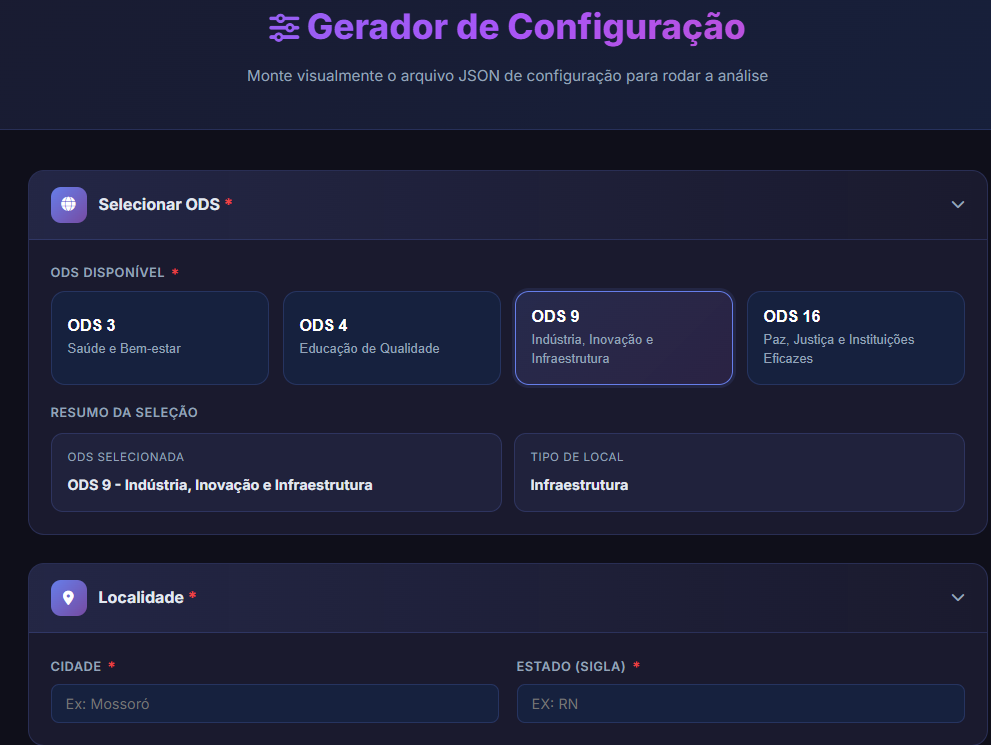
\includegraphics[width=0.70\textwidth]{figuras/formulario-config-ods}
    \legend{Fonte: Elaborado pelo autor (2026).}
\end{figure}

O fluxo de uso completo compreende quatro etapas:

\begin{enumerate}
    \item \textbf{Preenchimento}: o usuário seleciona o ODS, informa o município e ajusta dimensões, termos de busca e parâmetros de execução no formulário;
    \item \textbf{Geração}: ao confirmar, o formulário monta e disponibiliza para download o arquivo JSON de configuração, no mesmo formato dos arquivos descritos na Seção~\ref{subsec:v3};
    \item \textbf{Execução}: o arquivo gerado é passado ao motor genérico via     \item \textbf{Execução}: o arquivo gerado é passado ao motor genérico, que realiza coleta, filtragem, análise e geração de diagnósticos, por meio do comando:
\begin{verbatim}
python ods_analise_generica.py --config <arquivo>
\end{verbatim}
 que realiza coleta, filtragem, análise e geração de diagnósticos;
    \item \textbf{Visualização}: o JSON de análise resultante é carregado no dashboard unificado para exploração interativa dos resultados.
\end{enumerate}

Dessa forma, o ciclo completo de análise de um novo ODS ou município pode ser realizado sem escrever ou modificar uma única linha de código.

\section{Dashboards Web Públicos}
\label{sec:dashboards-publicos}

Inicialmente, os resultados foram estruturados em formato compatível com o Microsoft Power BI. No entanto, essa abordagem foi substituída por dashboards web desenvolvidos com HTML, CSS e JavaScript, visando reduzir a dependência de ferramentas proprietárias e facilitar o acesso público aos resultados. A versão final da interface utiliza Chart.js para geração de gráficos de distribuição de sentimentos e problemas por dimensão; Leaflet.js para recursos de visualização geográfica; WordCloud2.js para nuvens de palavras extraídas das análises; e Font Awesome para a composição visual dos ícones da interface.

Foram implementadas páginas específicas para o dashboard do ODS 9, dashboard do ODS 16 e páginas de diagnóstico textual para cada objetivo. A versão pública também inclui um dashboard unificado capaz de carregar arquivos JSON de análise por localidade, permitindo reutilizar a mesma interface para diferentes municípios e ODS, inclusive os arquivos gerados nas execuções de generalização descritos nas Seções~\ref{sec:generalizacao-multiplos-ods} e~\ref{sec:generalizacao-geografica}. Além disso, os dados de diagnóstico podem ser embutidos em arquivos JSON auxiliares, permitindo que as páginas sejam publicadas como arquivos estáticos, sem necessidade de servidor ou banco de dados.

Como os dashboards são compostos exclusivamente por arquivos estáticos, o conjunto foi publicado gratuitamente na plataforma Netlify e está disponível publicamente em \url{https://dashboard-ods-mossoro.netlify.app}. A versão hospedada inclui o dashboard unificado com os dados de Mossoró-RN, as páginas de diagnóstico dos ODS 9 e 16 e o formulário de geração de configurações descrito na Seção~\ref{sec:formulario-config}. Essa estratégia transformou a etapa de visualização em uma camada de apresentação leve, portátil e de fácil publicação, que também pode ser executada localmente em navegador, ampliando a acessibilidade da ferramenta para gestores públicos, pesquisadores e demais interessados.

	\chapter{Resultados}
\label{cap:resultados}

Este capítulo apresenta os resultados obtidos pela aplicação da metodologia proposta ao estudo de caso de Mossoró-RN, com foco nos ODS 9 (Indústria, Inovação e Infraestrutura) e ODS 16 (Paz, Justiça e Instituições Eficazes). Os dados foram coletados e analisados utilizando o sistema implementado, conforme descrito no capítulo anterior.

\section{Visão Geral da Coleta}
\label{sec:coleta-geral}

O sistema foi executado com o modelo Gemini 2.5 Flash como provedor principal de análise. A Tabela~\ref{tab:resumo-coleta} apresenta o resumo quantitativo da coleta realizada para os dois ODS.

\begin{table}[h!]
    \centering
    \caption{Resumo quantitativo da coleta de dados por ODS em Mossoró-RN}
    \label{tab:resumo-coleta}
    \begin{tabular}{lcc}
        \hline
        \textbf{Métrica} & \textbf{ODS 9} & \textbf{ODS 16} \\
        \hline
        Total de análises coletadas & 253 & 116 \\
        Estabelecimentos únicos analisados & 117 & 12 \\
        Problemas detectados & 144 & 54 \\
        Percentual de análises com problema & 56,9\% & 46,6\% \\
        Score médio de confiança & 0,87 & 0,84 \\
        \hline
    \end{tabular}
    \legend{Fonte: Elaborado pelo autor (2025).}
\end{table}

\section{ODS 9 -- Indústria, Inovação e Infraestrutura}
\label{sec:resultados-ods9}

\subsection{Distribuição por Tipo de Estabelecimento}
\label{subsec:tipos-ods9}

As 253 análises do ODS 9 foram coletadas em 117 estabelecimentos únicos, abrangendo sete categorias de locais relacionadas às dimensões do objetivo:

\begin{itemize}
    \item \textbf{Infraestrutura de transporte}: rodoviárias, aeroporto, terminais rodoviários, estações e paradas de ônibus;
    \item \textbf{Infraestrutura urbana}: ruas, avenidas, pontes, viadutos, pavimentação e iluminação pública;
    \item \textbf{Tecnologia e telecomunicações}: lojas de eletrônicos, operadoras de telefonia, provedores de internet e serviços de tecnologia;
    \item \textbf{Indústria}: fábricas, parques industriais e empresas de transformação;
    \item \textbf{Energia}: distribuidoras de energia elétrica e serviços de energia renovável;
    \item \textbf{Micro e pequenas empresas}: comércios locais, serviços de apoio ao empreendedorismo e instituições de crédito para pequenos negócios;
    \item \textbf{Inovação}: \textit{startups}, incubadoras e espaços de inovação.
\end{itemize}

Essa diversidade de tipos de local permitiu capturar percepções sobre todas as sete dimensões do ODS 9, desde ativos físicos de infraestrutura até o ambiente de negócios e inovação do município.

\subsection{Distribuição de Sentimentos}
\label{subsec:sentimentos-ods9}

Das 253 análises coletadas para o ODS 9, a distribuição de sentimentos revelou um cenário predominantemente negativo, conforme apresentado na Tabela~\ref{tab:sentimentos-ods9} e na Figura~\ref{fig:sentimentos-comparados}, que compara a distribuição de sentimentos entre os dois ODS analisados.

\begin{table}[h!]
    \centering
    \caption{Distribuição de sentimentos -- ODS 9 (Mossoró-RN)}
    \label{tab:sentimentos-ods9}
    \begin{tabular}{lcc}
        \hline
        \textbf{Sentimento} & \textbf{Quantidade} & \textbf{Percentual} \\
        \hline
        Positivo & 37 & 14,6\% \\
        Negativo & 103 & 40,7\% \\
        Neutro & 113 & 44,7\% \\
        \hline
        \textbf{Total} & \textbf{253} & \textbf{100\%} \\
        Contribuem para baixo ODS 9 & 144 & 56,9\% \\
        \hline
    \end{tabular}
    \legend{Fonte: Elaborado pelo autor (2025).}
\end{table}

\begin{figure}[h!]
    \centering
    \caption{Distribuição de sentimentos por ODS em Mossoró-RN}
    \label{fig:sentimentos-comparados}
    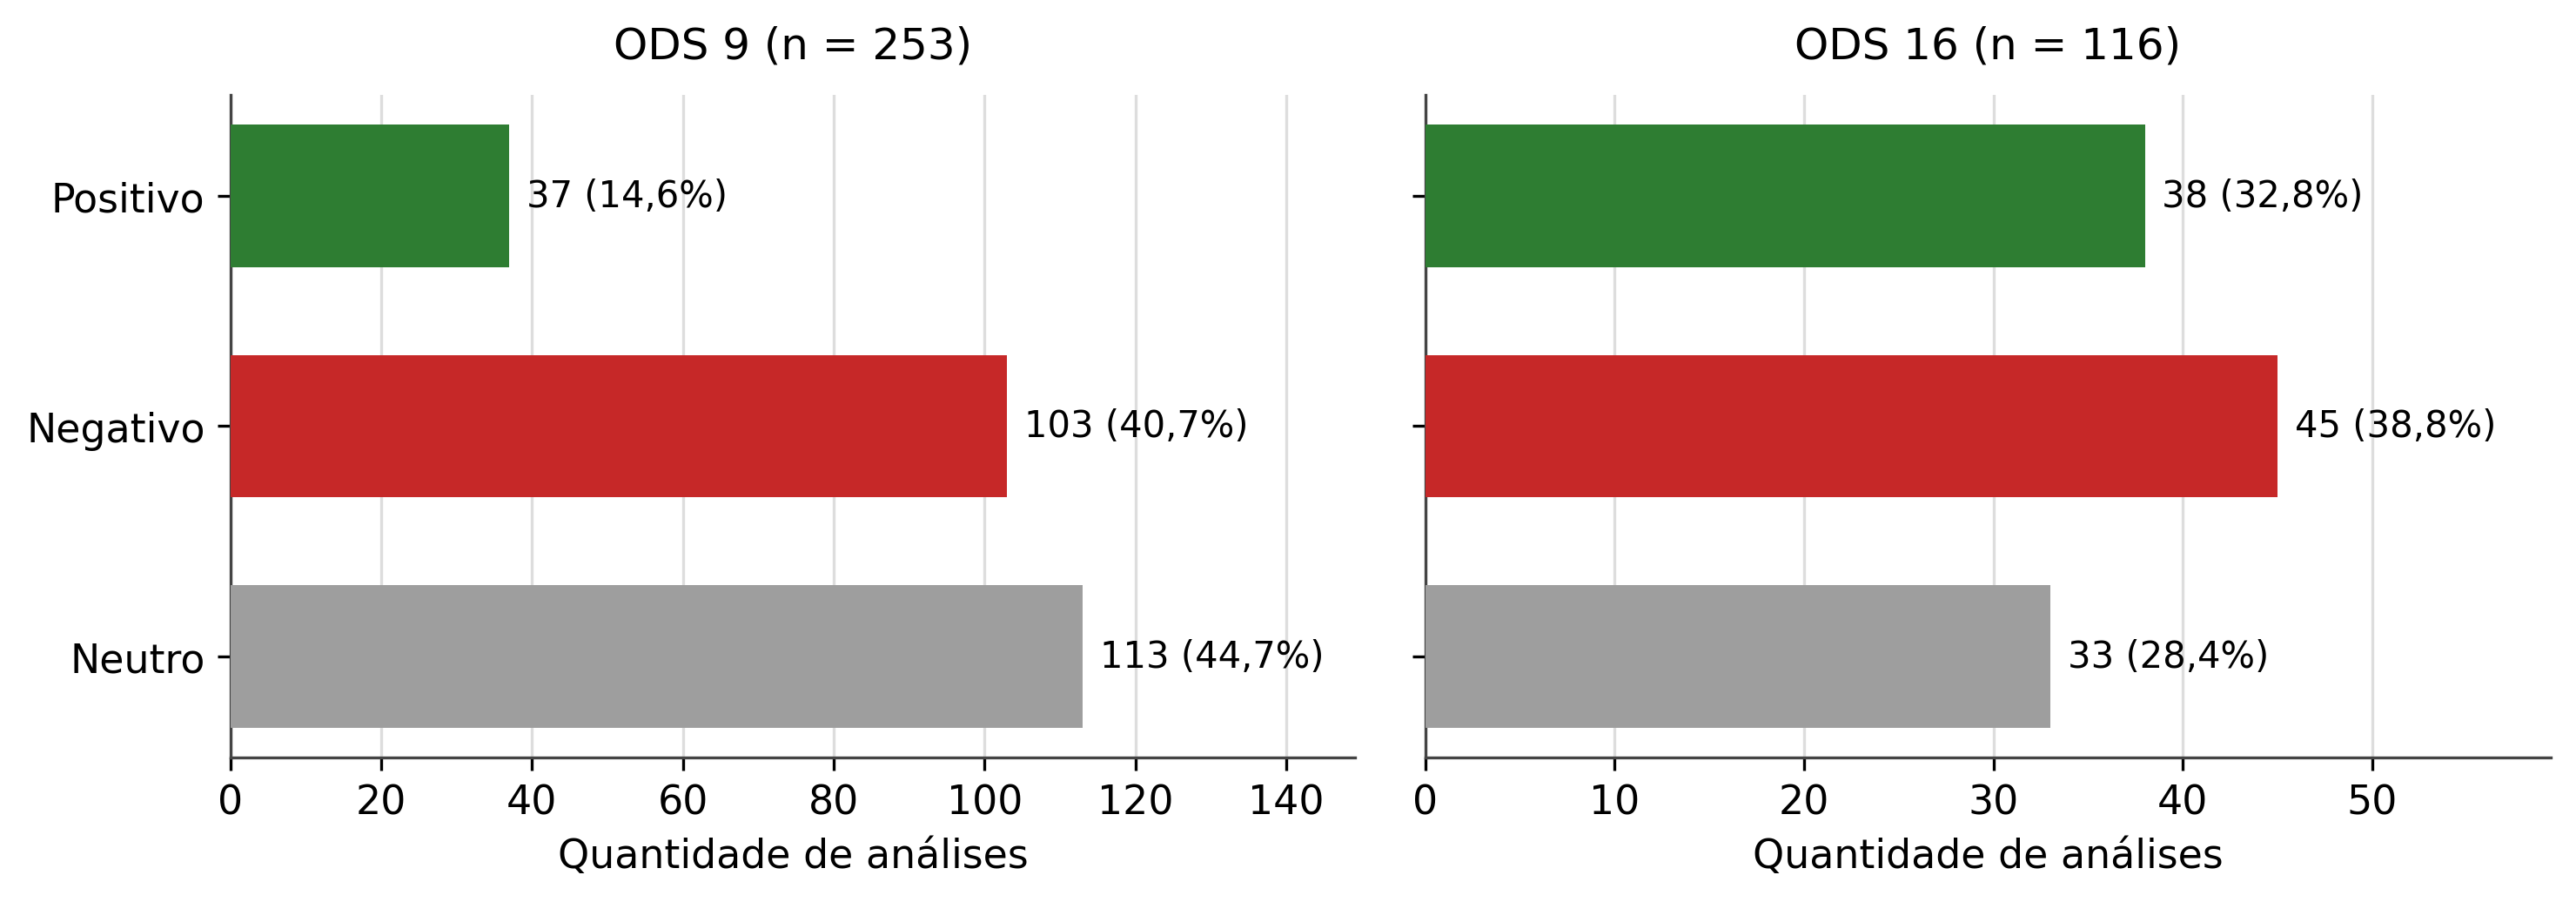
\includegraphics[width=0.95\textwidth]{figuras/distribuicao-sentimentos-ods}
    \legend{Fonte: Elaborado pelo autor (2026).}
\end{figure}

A baixa proporção de avaliações positivas (14,6\%) e o fato de que 56,9\% das análises contribuem diretamente para o baixo desempenho validam a pontuação muito baixa (0--39,99) atribuída a Mossoró no ODS 9 pelo IDSC \cite{idsc2024}. Os scores de confiança elevados (média de 0,87) indicam que o modelo identificou com segurança os aspectos problemáticos nos textos analisados.

A elevada taxa de comentários neutros (44,7\%) pode ser interpretada de duas formas complementares: por um lado, pode indicar relatos descritivos com baixo conteúdo avaliativo explícito; por outro, pode refletir uma normalização de problemas crônicos, em que deficiências recorrentes passam a ser percebidas como parte do cotidiano urbano. Essa leitura reforça a importância da análise por aspecto, uma vez que avaliações aparentemente neutras podem, ao serem analisadas semanticamente, revelar indícios de problemas persistentes.

\subsection{Distribuição de Problemas por Dimensão}
\label{subsec:problemas-ods9}

A Tabela~\ref{tab:problemas-ods9} apresenta a distribuição quantitativa de menções problemáticas por dimensão do ODS 9, extraída do campo de aspectos problemáticos identificados pela IA em cada análise.

\begin{table}[h!]
    \centering
    \caption{Distribuição de menções problemáticas por dimensão -- ODS 9 (Mossoró-RN)}
    \label{tab:problemas-ods9}
    \begin{tabular}{lcc}
        \hline
        \textbf{Dimensão} & \textbf{Menções} & \textbf{Percentual} \\
        \hline
        Infraestrutura Resiliente e Moderna & 85 & 33,6\% \\
        Transporte Público e Mobilidade & 54 & 21,3\% \\
        Acesso à Tecnologia e Informação & 52 & 20,6\% \\
        Valorização da Micro e Pequena Empresa & 48 & 19,0\% \\
        Industrialização Inclusiva e Sustentável & 37 & 14,6\% \\
        Inovação e Pesquisa & 30 & 11,9\% \\
        Eficiência Energética & 29 & 11,5\% \\
        \hline
    \end{tabular}
    \legend{Fonte: Elaborado pelo autor (2026). Percentuais calculados sobre as 253 análises; uma mesma análise pode mencionar problemas em mais de uma dimensão.}
\end{table}

A distribuição evidencia que os problemas do ODS 9 em Mossoró concentram-se nas dimensões físicas e econômicas de base, detalhadas a seguir:

\textbf{Infraestrutura Resiliente e Moderna (85 menções -- 33,6\%)}: dimensão mais problemática do conjunto. O Terminal Rodoviário de Mossoró emergiu como o principal foco de problemas: as avaliações descrevem um equipamento em estado crítico de deterioração, com estruturas abandonadas, risco de queda, condições insalubres (banheiros imundos, ausência de limpeza), iluminação inadequada e falta de manutenção preventiva. A totalidade dos comentários sobre o terminal classificou a infraestrutura como negativa, com scores de confiança acima de 0,85.

\textbf{Transporte Público e Mobilidade (54 menções -- 21,3\%)}: as avaliações do terminal rodoviário e de paradas de ônibus apontam para um sistema de transporte público em colapso: ausência de serviços básicos essenciais, falta de controle sanitário, experiência do usuário altamente comprometida e conectividade regional prejudicada.

\textbf{Acesso à Tecnologia e Informação (52 menções -- 20,6\%)}: as queixas concentram-se em operadoras de telefonia e provedores de internet, com relatos de instabilidade do serviço, atendimento deficiente e cobertura desigual entre regiões da cidade.

\textbf{Valorização da Micro e Pequena Empresa (48 menções -- 19,0\%)}: as análises revelam ausência de comércios básicos em locais estratégicos, limitadas oportunidades para pequenos negócios e insuficiência de suporte ao empreendedorismo local. É a dimensão com maior número absoluto de menções nas avaliações (171 análises a mencionam), refletindo o peso do comércio local na amostra.

As dimensões de Industrialização (14,6\%), Inovação e Pesquisa (11,9\%) e Eficiência Energética (11,5\%) apresentaram menor volume de menções problemáticas, em parte pela menor presença desses tipos de estabelecimento na amostra coletada. Em termos de localização, os estabelecimentos com maior concentração de análises problemáticas foram a Rodoviária de Mossoró, o Terminal Rodoviário Diram Ramos do Amaral, o Aeroporto Dix-Sept Rosado e a Secretaria Municipal de Infraestrutura, Meio Ambiente, Urbanismo e Serviços Urbanos, reforçando o padrão de concentração de problemas em equipamentos de transporte e órgãos de gestão urbana.

\subsection{Dashboard ODS 9}
\label{subsec:dashboard-ods9}

A Figura~\ref{fig:dashboard-ods9} apresenta o dashboard web desenvolvido para visualização dos resultados do ODS 9. A interface substitui a abordagem inicialmente prevista em Microsoft Power BI por uma solução HTML, CSS e JavaScript, acessível diretamente pelo navegador.

\begin{figure}[h!]
    \centering
    \caption{Dashboard web -- ODS 9: Indústria, Inovação e Infraestrutura em Mossoró-RN}
    \label{fig:dashboard-ods9}
    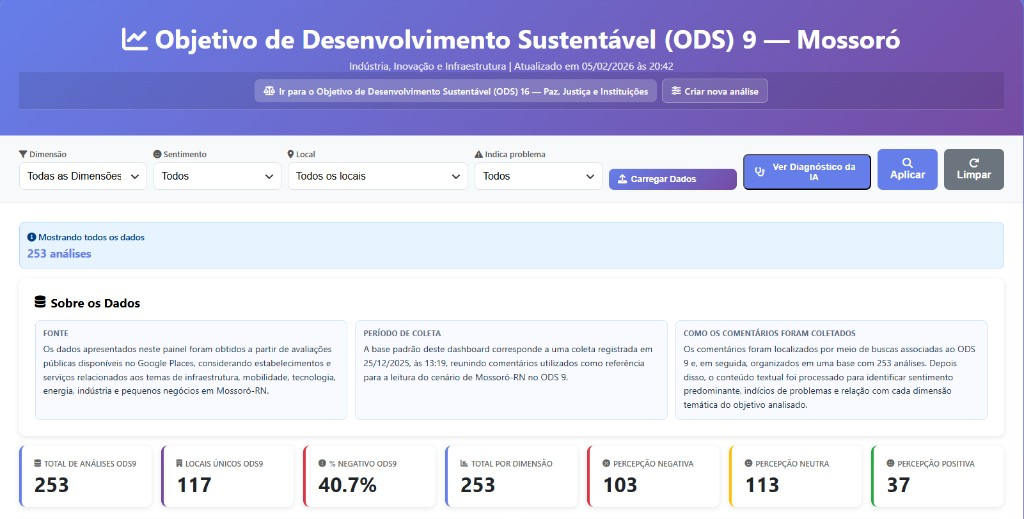
\includegraphics[width=0.95\textwidth]{figuras/dashboard-web-ods9}
    \legend{Fonte: Elaborado pelo autor (2025).}
\end{figure}

O dashboard possibilita filtragem dinâmica por dimensão, sentimento, local e indicação de problema, além da visualização de métricas consolidadas, cards informativos e acesso direto ao diagnóstico gerado pela IA. Essa organização facilita a leitura dos resultados por gestores públicos e especialistas, sem exigir conhecimento prévio em ferramentas proprietárias de inteligência de negócios.

\section{ODS 16 -- Paz, Justiça e Instituições Eficazes}
\label{sec:resultados-ods16}

\subsection{Composição da Amostra}
\label{subsec:amostra-ods16}

Para o ODS 16, foram coletadas 116 análises válidas distribuídas entre 12 estabelecimentos únicos. Embora aparentemente pequena, essa amostra representa os principais órgãos de justiça e segurança pública de Mossoró-RN, incluindo:

\begin{itemize}
    \item \textbf{Órgãos de segurança pública}: delegacias, polícia militar, guarda civil municipal e batalhões;
    \item \textbf{Poder judiciário}: fóruns, tribunais, defensoria pública e Ministério Público;
    \item \textbf{Instituições públicas}: prefeitura, secretarias municipais e câmara municipal;
    \item \textbf{Órgãos eleitorais}: TRE e Justiça Eleitoral;
    \item \textbf{Espaços públicos}: praças e parques, quando as avaliações mencionam segurança ou insegurança.
\end{itemize}

A amostra de 12 estabelecimentos reflete a realidade institucional do município: Mossoró possui um número limitado de órgãos públicos de justiça e segurança formalmente cadastrados na Google Places API, e o sistema capturou os principais estabelecimentos disponíveis. Essa cobertura dos órgãos institucionais relevantes garante que as análises representem adequadamente as percepções sobre o ODS 16 na cidade, ainda que o número absoluto de locais seja menor do que o do ODS 9, que inclui também estabelecimentos comerciais e de infraestrutura.

\subsection{Distribuição de Sentimentos}
\label{subsec:sentimentos-ods16}

A distribuição de sentimentos revela um padrão polarizado, conforme a Tabela~\ref{tab:sentimentos-ods16}. A comparação com o ODS 9, apresentada na Figura~\ref{fig:sentimentos-comparados}, evidencia diferenças relevantes no padrão de avaliação: enquanto o ODS 9 é dominado por avaliações neutras e negativas, o ODS 16 apresenta maior proporção de avaliações positivas, convivendo com queixas concentradas em dimensões críticas.

\begin{table}[h!]
    \centering
    \caption{Distribuição de sentimentos -- ODS 16 (Mossoró-RN)}
    \label{tab:sentimentos-ods16}
    \begin{tabular}{lcc}
        \hline
        \textbf{Sentimento} & \textbf{Quantidade} & \textbf{Percentual} \\
        \hline
        Positivo & 38 & 32,8\% \\
        Negativo & 45 & 38,8\% \\
        Neutro & 33 & 28,4\% \\
        \hline
        \textbf{Total} & \textbf{116} & \textbf{100\%} \\
        Contribuem para baixo ODS 16 & 54 & 46,6\% \\
        \hline
    \end{tabular}
    \legend{Fonte: Elaborado pelo autor (2025).}
\end{table}

Embora a proporção de avaliações positivas (32,8\%) seja maior do que no ODS 9, a concentração de problemas em dimensões críticas -- especialmente instituições eficazes (37,1\% das análises) e segurança pública (11,2\%) -- é suficiente para manter a pontuação na faixa muito baixa. Esse resultado é coerente com a natureza do ODS 16, no qual a experiência do cidadão é influenciada pela qualidade do atendimento, pela eficiência administrativa e pela transparência dos processos, elementos que tendem a gerar avaliações mais emocionalmente carregadas do que as associadas a infraestruturas físicas.

\subsection{Distribuição de Problemas por Dimensão}
\label{subsec:dimensoes-ods16}

A Tabela~\ref{tab:problemas-ods16} apresenta a distribuição quantitativa de menções de problemas por dimensão do ODS 16, e a Figura~\ref{fig:problemas-dimensao-ods16} evidencia graficamente a assimetria entre a dimensão dominante e as demais.

\begin{table}[h!]
    \centering
    \caption{Distribuição de problemas por dimensão -- ODS 16 (Mossoró-RN)}
    \label{tab:problemas-ods16}
    \begin{tabular}{lcc}
        \hline
        \textbf{Dimensão} & \textbf{Menções} & \textbf{Percentual} \\
        \hline
        Instituições Eficazes e Responsáveis & 43 & 37,1\% \\
        Direitos Humanos e Estado de Direito & 14 & 12,1\% \\
        Segurança Pública e Redução da Violência & 13 & 11,2\% \\
        Acesso à Justiça & 12 & 10,3\% \\
        Transparência e Combate à Corrupção & 8 & 6,9\% \\
        Participação Cidadã e Accountability & 6 & 5,2\% \\
        Proteção de Crianças e Grupos Vulneráveis & 6 & 5,2\% \\
        \hline
    \end{tabular}
    \legend{Fonte: Elaborado pelo autor (2025). Percentuais calculados sobre as 116 análises; uma mesma análise pode mencionar problemas em mais de uma dimensão.}
\end{table}

\begin{figure}[h!]
    \centering
    \caption{Distribuição de problemas por dimensão -- ODS 16 (Mossoró-RN)}
    \label{fig:problemas-dimensao-ods16}
    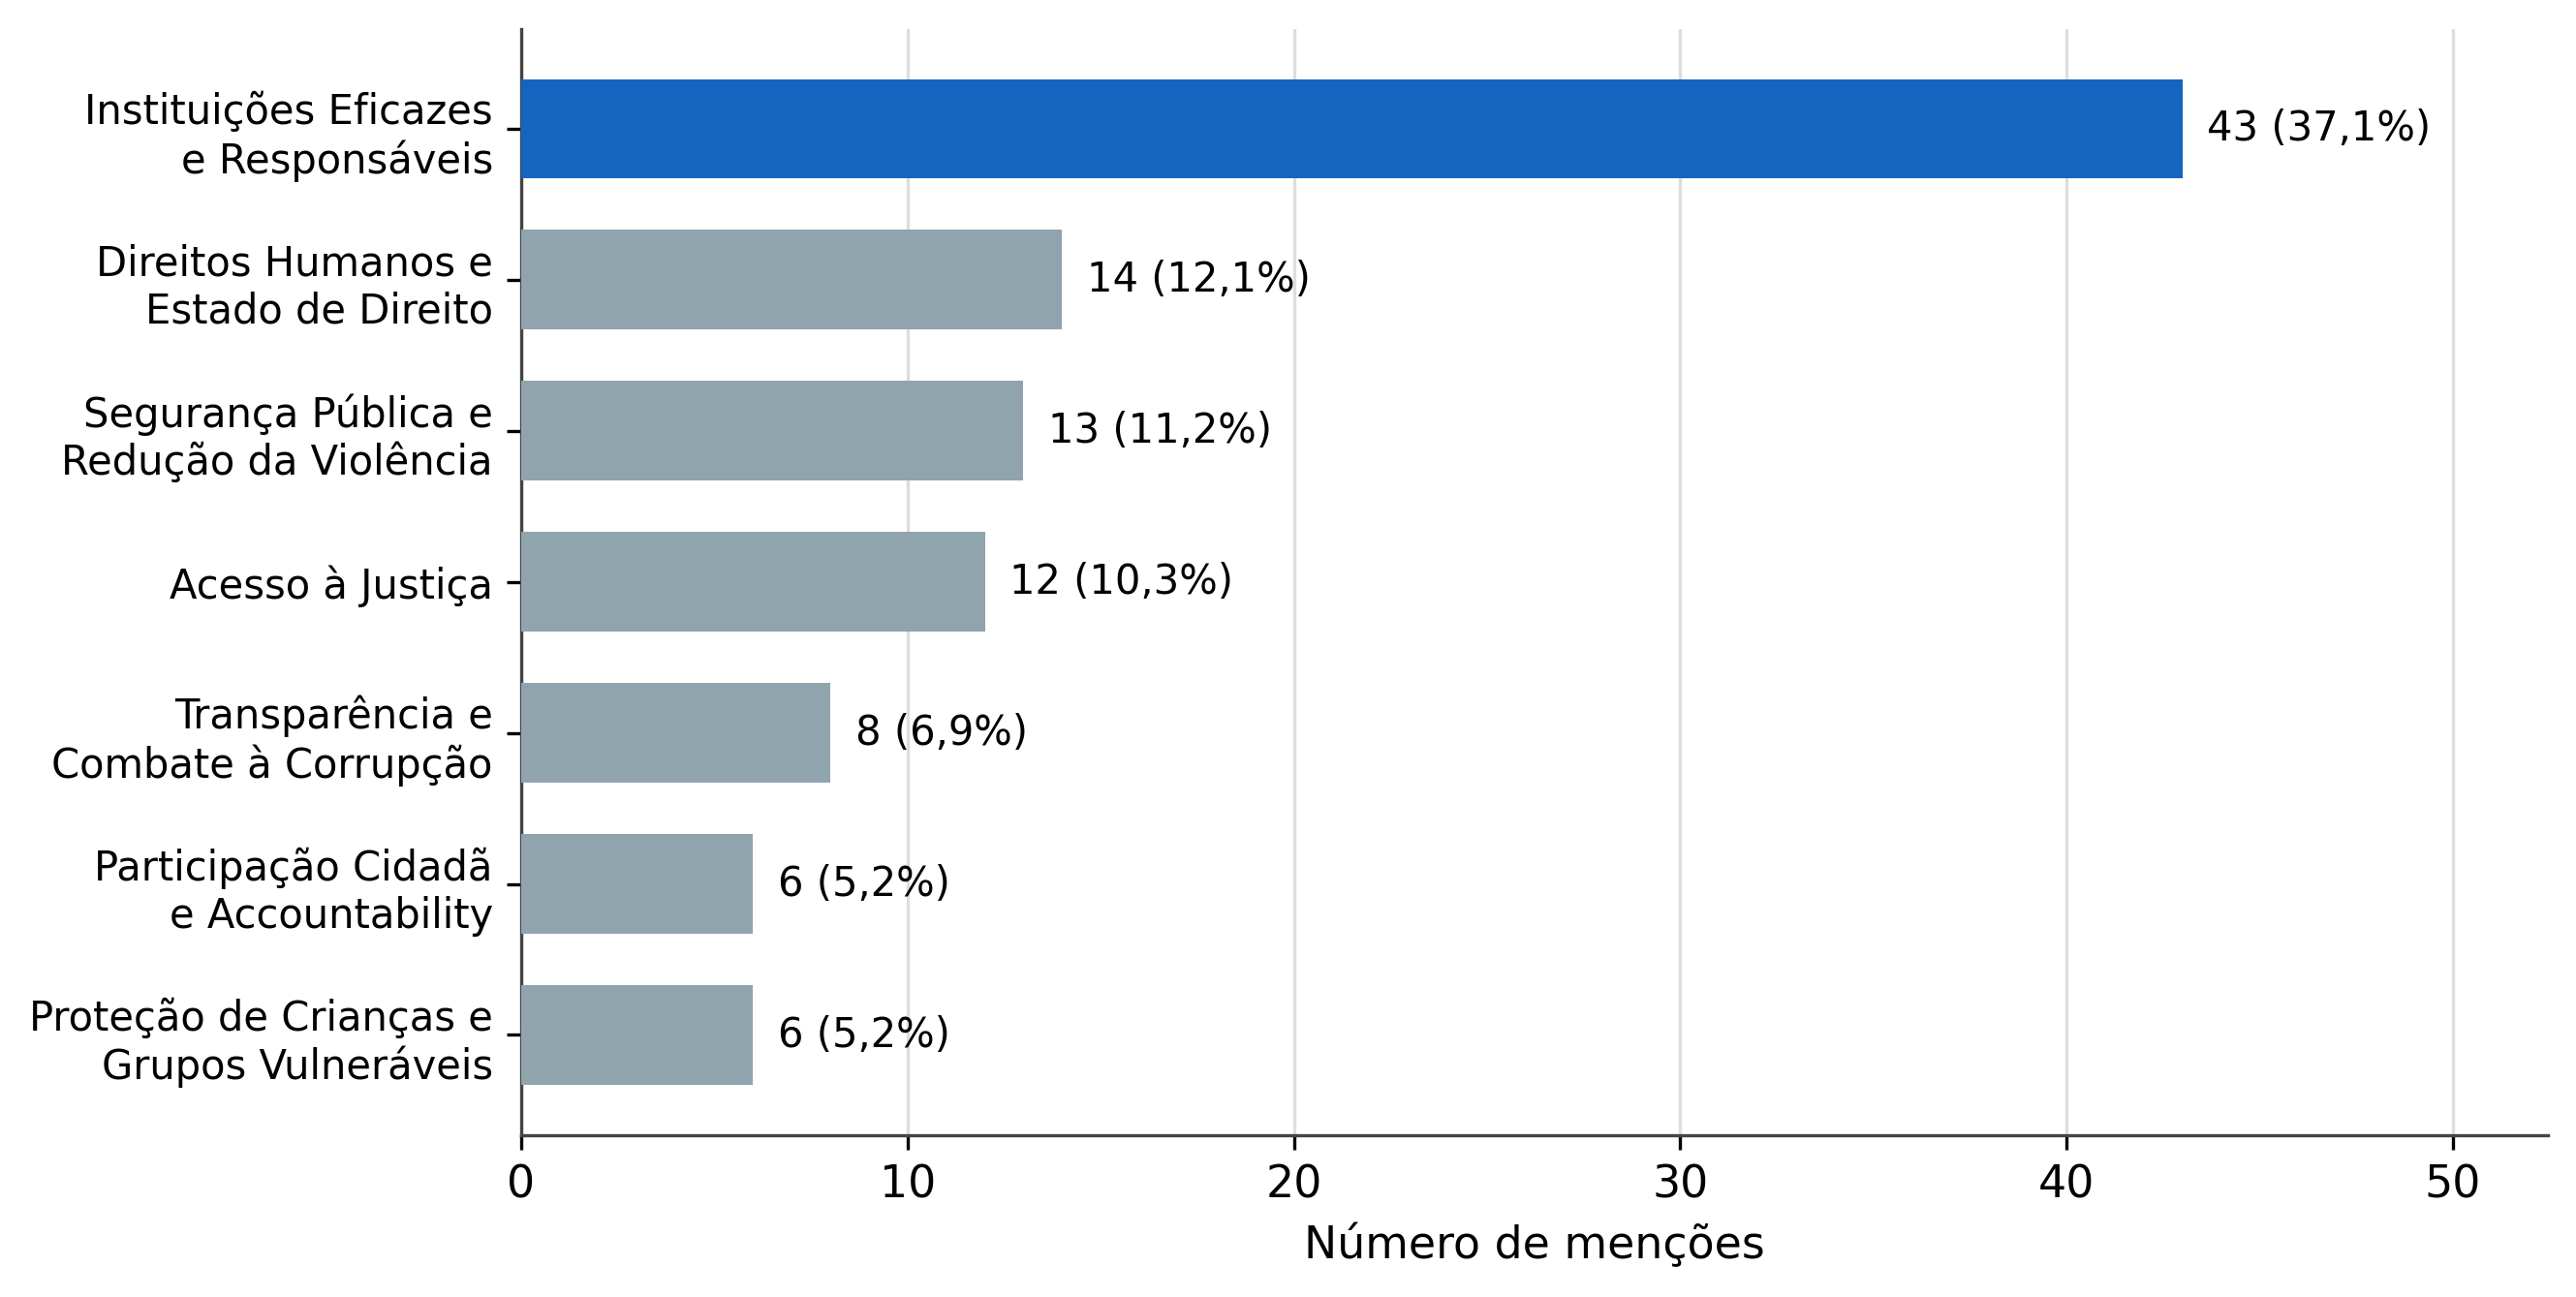
\includegraphics[width=0.90\textwidth]{figuras/problemas-dimensao-ods16}
    \legend{Fonte: Elaborado pelo autor (2026).}
\end{figure}

A dimensão \textit{Instituições Eficazes e Responsáveis} domina o conjunto de problemas (37,1\% das menções), evidenciando que a ineficiência administrativa é a raiz da maioria dos problemas identificados para o ODS 16 em Mossoró. Os principais problemas relatados nesta dimensão incluem: atendimento demorado e burocrático em secretarias municipais, insuficiência de pessoal, piora do atendimento com a migração para canais digitais e deficiências de gestão.

As demais dimensões reforçam esse quadro de fragilidade institucional. \textit{Direitos Humanos e Estado de Direito} registrou 14 menções (12,1\%), evidenciando violações em contextos de fiscalização e necessidade de capacitação. \textit{Segurança Pública e Redução da Violência} somou 13 menções (11,2\%), associadas à atuação insuficiente dos órgãos de segurança e à sensação de insegurança. \textit{Acesso à Justiça} (12 menções -- 10,3\%) relacionou-se à burocracia excessiva e a dificuldades de atendimento presencial. \textit{Transparência e Combate à Corrupção} (6,9\%), \textit{Participação Cidadã e Accountability} (5,2\%) e \textit{Proteção de Crianças e Grupos Vulneráveis} (5,2\%) completam o quadro de fragilidades identificadas.

\subsection{Dashboard ODS 16}
\label{subsec:dashboard-ods16}

A Figura~\ref{fig:dashboard-ods16} apresenta o dashboard web para o ODS 16, que permite exploração interativa dos 116 registros coletados.

\begin{figure}[h!]
    \centering
    \caption{Dashboard web -- ODS 16: Paz, Justiça e Instituições Eficazes em Mossoró-RN}
    \label{fig:dashboard-ods16}
    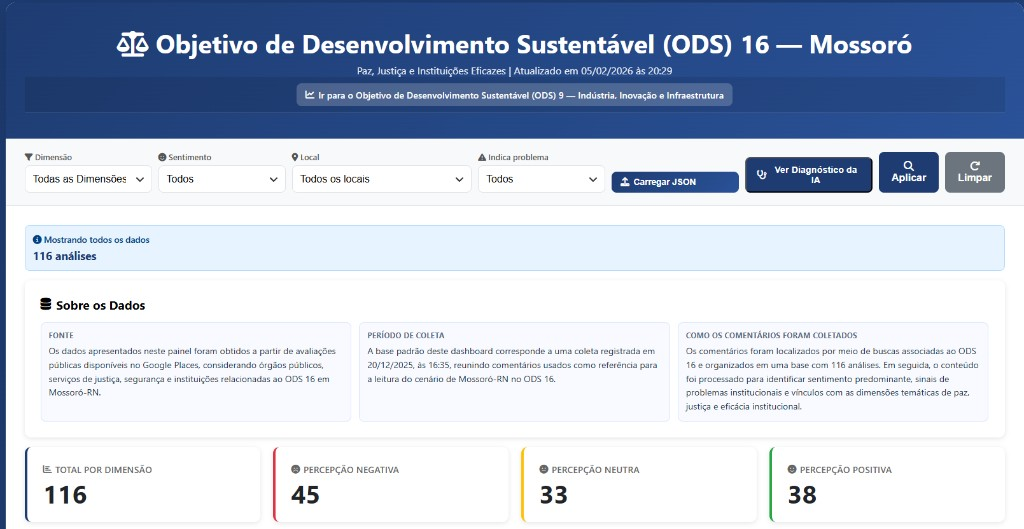
\includegraphics[width=0.95\textwidth]{figuras/dashboard-web-ods16}
    \legend{Fonte: Elaborado pelo autor (2025).}
\end{figure}

\section{Diagnósticos Gerados Automaticamente}
\label{sec:diagnosticos-automaticos}

O sistema gerou diagnósticos estruturados em linguagem natural para cada ODS, sintetizando os padrões identificados nas análises individuais. Cada diagnóstico é composto por seis blocos: diagnóstico geral do baixo desempenho, análise por dimensão, pontos críticos prioritários, impacto social e urbano, recomendações estratégicas e conclusão. Para o ODS 9, o diagnóstico identificou a degradação da infraestrutura física -- especialmente o Terminal Rodoviário -- como gargalo central, com impacto em cascata sobre o transporte público, a mobilidade urbana e a economia local. Para o ODS 16, o diagnóstico apontou a fragilidade institucional sistêmica como causa-raiz, amplificando problemas em segurança pública, acesso à justiça e direitos humanos.

A seguir, apresenta-se um trecho representativo do diagnóstico gerado para cada ODS, transcrito do campo \texttt{conclusao\_geral\_diagnostico} dos arquivos JSON de resultados. Para o ODS 9, o diagnóstico geral e o trecho da análise dimensional de infraestrutura ilustram a capacidade do sistema de articular os indicadores quantitativos com as evidências qualitativas extraídas das avaliações:

\begin{citacao}
A análise de 253 avaliações coletadas sobre Mossoró-RN revela que 144 análises (56,9\%) identificam problemas que contribuem diretamente para o baixo desempenho no ODS 9 (pontuação muito baixa: 0--39,99). A distribuição de sentimentos mostra predominância negativa: 103 análises negativas (40,7\%), 113 neutras (44,7\%) e apenas 37 positivas (14,6\%). Esta distribuição evidencia um cenário crítico de infraestrutura, inovação e desenvolvimento industrial na cidade. [...] Infraestrutura Resiliente e Moderna: os problemas mais frequentes incluem infraestrutura deteriorada, falta de manutenção, estacionamentos inadequados, banheiros em estado deplorável e necessidade urgente de reformas. A rodoviária de Mossoró é descrita como ``cenário pós-apocalíptico'', com estruturas abandonadas, sujas e em risco de colapso. Ruas precisam de reformas urgentes e há falta de serviços básicos em terminais e espaços públicos. (Diagnóstico gerado automaticamente pelo sistema, 2025)
\end{citacao}

Para o ODS 16, o trecho selecionado evidencia a identificação da fragilidade institucional como causa central do baixo desempenho:

\begin{citacao}
Mossoró-RN apresenta pontuação \textit{muito baixa} no ODS 16 (0--39,99) pautada por percepção pública amplamente crítica sobre a capacidade institucional e pelo registro significativo de análises que vinculam falhas institucionais à fragilização da paz e da justiça; das 116 análises, 54 (46,6\%) foram identificadas como contributivas para o baixo desempenho no ODS 16, com 43 menções explícitas a \textit{instituições eficazes} como problema central. [...] Instituições Eficazes e Responsáveis: esta é a dimensão mais citada (43 menções) e apresenta as falhas mais determinantes para o desempenho baixo: ineficiência no atendimento público, piora do serviço em migração para canais digitais, insuficiência de pessoal, deficiências de gestão em secretarias e falta de escalabilidade de práticas eficazes. As análises indicam baixa confiança institucional e fragilidade administrativa que comprometem implementação de políticas, execução de serviços essenciais e resposta a demandas cidadãs. (Diagnóstico gerado automaticamente pelo sistema, 2025)
\end{citacao}

Os trechos ilustram duas características relevantes da geração automatizada: a fidelidade aos números agregados da coleta, reproduzidos corretamente nos textos, e a incorporação de evidências textuais extraídas diretamente das avaliações dos cidadãos, como a descrição da rodoviária. Os diagnósticos gerados foram validados por comparação com os problemas identificados manualmente na literatura e em relatórios de organismos oficiais. A consistência entre os achados automatizados e as evidências conhecidas confirma a capacidade do sistema de produzir diagnósticos confiáveis a partir de dados não estruturados.

A Figura~\ref{fig:diagnostico-ods9} ilustra a página de diagnóstico textual do ODS 9, na qual o usuário pode consultar o diagnóstico geral e os diagnósticos por dimensão. A página organiza o texto produzido pela IA em uma interface de leitura própria, separando a exploração quantitativa do dashboard da análise qualitativa gerada automaticamente.

\begin{figure}[H]
    \centering
    \caption{Página web de diagnóstico automatizado -- ODS 9}
    \label{fig:diagnostico-ods9}
    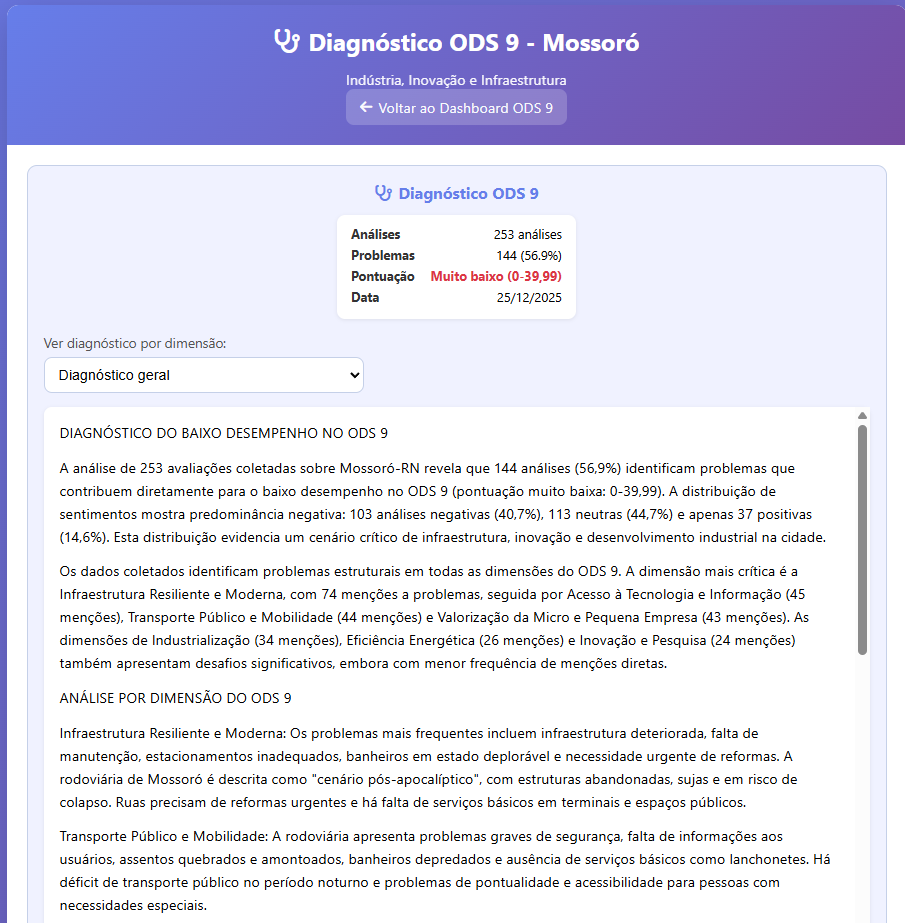
\includegraphics[width=0.70\textwidth]{figuras/diagnostico-web-ods9}
    \legend{Fonte: Elaborado pelo autor (2025).}
\end{figure}
\FloatBarrier
\section{Evidências de Generalização da Abordagem}
\label{sec:generalizacao-abordagem}

Embora o estudo de caso principal desta dissertação concentre-se em Mossoró-RN, com ênfase nos ODS 9 e 16, a implementação também foi avaliada quanto à sua capacidade de generalização para outros objetivos e municípios. Essa verificação foi realizada por meio da execução do motor de análise em diferentes combinações de ODS, cidade e conjunto de dimensões, mantendo a mesma lógica de coleta, filtragem, análise por aspecto, geração de JSON e produção de diagnóstico automatizado.

A generalização foi testada em dois níveis. No primeiro, os modelos específicos de ODS foram reaplicados em outras cidades (Natal-RN, Fortaleza-CE, João Pessoa-PB e Salvador-BA), mantendo a estrutura de análise definida para cada objetivo. No segundo, a versão genérica orientada por arquivos de configuração JSON foi executada sem alteração do código-fonte para os ODS 3 e 4, modificando apenas os parâmetros de entrada relativos ao ODS, à localidade, às dimensões e aos termos de busca. Os detalhes operacionais dessas execuções, incluindo os arquivos de configuração utilizados e os volumes coletados, são apresentados nas Seções~\ref{sec:generalizacao-multiplos-ods} e~\ref{sec:generalizacao-geografica}.

Essas execuções não substituem o estudo de caso aprofundado realizado em Mossoró-RN, mas demonstram que a arquitetura proposta não está rigidamente acoplada a um único município ou a um único ODS. A possibilidade de alterar o arquivo de configuração e reaplicar a pipeline a novos contextos constitui uma evidência técnica de escalabilidade. Assim, a abordagem pode ser replicada para outros municípios brasileiros, desde que existam avaliações públicas disponíveis na Google Places API e que as dimensões do ODS analisado sejam adequadamente parametrizadas.

É importante destacar que a generalização aqui apresentada é de natureza técnica e operacional. Ou seja, demonstra que o sistema executa a coleta, a filtragem, a análise e a geração de diagnósticos em diferentes contextos. A generalização substantiva dos achados -- isto é, a afirmação de que os mesmos problemas identificados em Mossoró ocorrem em outras cidades -- requer estudos comparativos adicionais, com validação local e análise das especificidades urbanas, institucionais e socioeconômicas de cada município.

\section{Correlações entre Dimensões e Padrões Transversais}
\label{sec:correlacoes}

A análise comparativa entre os dois ODS revelou padrões estruturais comuns que transcendem as especificidades de cada objetivo:

\begin{itemize}
    \item \textbf{Falta de manutenção preventiva}: tanto a infraestrutura física (ODS 9) quanto os serviços institucionais (ODS 16) degradam-se por ausência de manutenção e monitoramento contínuos;
    \item \textbf{Insuficiência de recursos humanos e financeiros}: ambos os ODS sofrem com quadros de pessoal reduzidos e orçamento insuficiente para atender a demanda;
    \item \textbf{Desconexão com necessidades cidadãs}: os serviços públicos analisados mostram baixa capacidade de resposta às demandas da população, evidenciada nas avaliações;
    \item \textbf{Concentração geográfica de problemas}: os estabelecimentos com maior número de avaliações negativas concentram-se no centro e em terminais de transporte, sugerindo prioridades claras de intervenção.
\end{itemize}

Para o ODS 16, a análise identificou uma cadeia causal entre as dimensões: instituições ineficazes amplificam barreiras ao acesso à justiça, que por sua vez contribuem para violações de direitos humanos e redução da participação cidadã, retroalimentando a fragilidade institucional.

	\chapter{Discussão}
\label{cap:discussao}

Este capítulo interpreta os resultados apresentados nos Capítulos~\ref{cap:resultados} e~\ref{cap:validacao-tam} à luz da literatura revisada e do problema de pesquisa. A discussão organiza-se em torno de cinco eixos: a leitura dos resultados quantitativos da análise de sentimentos em Mossoró-RN, com destaque para o significado do padrão de neutralidade observado no ODS 9; a estabilidade dos padrões identificados quando a abordagem foi generalizada para outros municípios e outros objetivos; a triangulação entre a avaliação de aceitação tecnológica e os resultados quantitativos produzidos pelos dashboards; as limitações que delimitam o alcance das conclusões; e, por fim, as implicações dos achados para o conceito de Cidades Inteligentes e para a prática da gestão pública municipal. Antes de tratar dessas implicações, a metodologia é confrontada com os trabalhos relacionados, de modo a situar a contribuição da pesquisa no estado da arte.

\section{Discussão dos Resultados Quantitativos}
\label{sec:disc-quantitativos}

Os resultados obtidos para Mossoró-RN reforçam a premissa central desta pesquisa: avaliações públicas georreferenciadas podem ser utilizadas como fonte complementar de informação para a análise do desempenho dos ODS em nível municipal. Diferentemente de indicadores oficiais, que apresentam caráter agregado e atualização periódica limitada, os dados perceptivos analisados refletem experiências diretas dos cidadãos com serviços, infraestruturas e instituições específicas. Nesse sentido, a metodologia proposta não deve ser interpretada como um mecanismo de validação causal do desempenho dos ODS, mas como um instrumento exploratório e analítico, capaz de revelar padrões, gargalos recorrentes e sinais precoces de problemas urbanos e institucionais.

\subsection{O Padrão de Neutralidade no ODS 9: a Normalização de Problemas Crônicos}
\label{subsec:disc-neutros-ods9}

Um dos achados mais instigantes da análise quantitativa diz respeito à distribuição de sentimentos do ODS 9, marcada por uma elevada proporção de avaliações negativas (40,7\%) e, sobretudo, neutras (44,7\%), com apenas 14,6\% de avaliações positivas. A predominância simultânea de relatos negativos e neutros sugere um cenário de insatisfação estrutural associado à infraestrutura urbana e aos serviços de transporte. Contudo, é a elevada taxa de comentários neutros que merece interpretação mais cuidadosa, pois ela pode ser lida de duas formas complementares.

Por um lado, a neutralidade pode indicar relatos meramente descritivos, com baixo conteúdo avaliativo explícito -- comentários que registram a existência ou a localização de um equipamento sem emitir juízo de valor direto. Por outro lado, e de forma mais reveladora, a neutralidade pode refletir um processo de \textit{normalização de problemas crônicos}: deficiências recorrentes que, por sua persistência ao longo do tempo, deixam de ser percebidas como anomalias e passam a ser tratadas como parte esperada do cotidiano urbano. Sob essa leitura, o cidadão que descreve sem indignação um terminal rodoviário deteriorado não o faz por satisfação, mas porque a degradação tornou-se o estado de referência contra o qual a experiência é avaliada. A ausência de afeto explícito, nesse caso, é em si um sintoma da gravidade e da cronicidade do problema.

Essa interpretação tem consequências metodológicas importantes. Uma análise de sentimentos restrita à polaridade global classificaria a maior parte dessas avaliações como neutras e, consequentemente, subestimaria a extensão dos problemas de infraestrutura. É precisamente aqui que a opção por uma análise baseada em aspectos (\textit{aspect-based sentiment analysis}) demonstra seu valor: ao decompor cada avaliação nas sete dimensões do ODS 9 e ao identificar explicitamente menções problemáticas, o sistema recupera, de comentários aparentemente neutros, indícios de fragilidades persistentes que escapariam a uma classificação superficial. O fato de 56,9\% das análises contribuírem diretamente para o baixo desempenho -- proporção superior à dos comentários explicitamente negativos -- evidencia que parte substancial dos problemas foi extraída justamente de avaliações que a polaridade global não capturaria como negativas. Esse resultado corrobora a observação de \citeauthor{wankhade2022} \citeyear{wankhade2022} sobre os limites das abordagens baseadas exclusivamente em polaridade e reforça a pertinência de modelos generativos capazes de inferir aspectos implícitos no texto, conforme demonstrado por \citeauthor{agua2025} \citeyear{agua2025}.

\subsection{A Polarização no ODS 16: a Centralidade da Eficiência Institucional}
\label{subsec:disc-ods16}

O ODS 16 apresentou um padrão distinto, caracterizado por maior polarização entre avaliações positivas e negativas. Embora 32,8\% das análises tenham sido classificadas como positivas -- proporção mais que duas vezes superior à do ODS 9 --, a frequência e a recorrência de relatos negativos em dimensões críticas, especialmente instituições eficazes, acesso à justiça e segurança pública, foram suficientes para sustentar a pontuação muito baixa atribuída ao município. Esse contraste entre os dois objetivos é coerente com a natureza dos serviços avaliados: enquanto o ODS 9 se ancora em ativos físicos cuja degradação é contínua e cumulativa, o ODS 16 depende da qualidade do atendimento, da eficiência administrativa e da transparência dos processos -- elementos que tendem a gerar experiências mais episódicas e, portanto, avaliações mais emocionalmente carregadas, ora muito positivas, ora muito negativas.

A dominância da dimensão \textit{Instituições Eficazes e Responsáveis}, que concentrou 37,1\% das menções problemáticas, é o achado mais relevante para o desenho de políticas públicas. Ele indica que, em Mossoró, o principal fator explicativo do baixo ODS 16 não é a violência ou a impunidade em sentido estrito, mas a qualidade do serviço público -- atendimento demorado e burocrático, insuficiência de pessoal, piora percebida com a migração para canais digitais e deficiências de gestão. As correlações identificadas entre as dimensões sugerem a existência de efeitos sistêmicos: relatos de ineficiência institucional associam-se frequentemente a dificuldades de acesso à justiça, enquanto menções a violações de direitos tendem a coexistir com percepções de baixa transparência e de \textit{accountability}. Esses padrões reforçam a natureza transversal do ODS 16 e indicam que falhas institucionais não ocorrem de forma isolada, mas se propagam por diferentes esferas da governança pública. Tal leitura está alinhada à argumentação de \citeauthor{massey2022} \citeyear{massey2022} sobre a interdependência entre boa governança e o avanço da Agenda 2030.

\subsection{Padrões Transversais e Concentração Geográfica}
\label{subsec:disc-transversais}

A análise comparativa entre os dois objetivos revelou padrões estruturais comuns que transcendem suas especificidades: a falta de manutenção preventiva, a insuficiência de recursos humanos e financeiros, e a desconexão entre os serviços públicos e as necessidades cidadãs. A degradação por ausência de manutenção contínua afeta tanto a infraestrutura física (ODS 9) quanto os serviços institucionais (ODS 16), sugerindo que a fragilidade não é setorial, mas característica de um modelo de gestão reativo, em que a intervenção ocorre apenas após o colapso.

A dimensão geográfica acrescenta uma camada acionável a esses achados. A concentração de problemas em áreas centrais -- onde se localizam os órgãos públicos com maior volume de demanda --, em terminais de transporte e em regiões periféricas associadas à percepção de insegurança, evidencia que os problemas urbanos e institucionais possuem hotspots identificáveis. Essa característica é particularmente relevante para o ODS 9, no qual os problemas identificados estão fortemente vinculados a ativos físicos concretos, como o Terminal Rodoviário de Mossoró, repetidamente apontado como o principal foco de avaliações negativas. A possibilidade de associar percepções diretamente a locais específicos constitui uma vantagem da fonte georreferenciada e habilita a priorização espacial de intervenções, tema retomado na Seção~\ref{sec:disc-implicacoes}.

\section{Discussão da Generalização da Abordagem}
\label{sec:disc-generalizacao}

As evidências de generalização apresentadas nas Seções~\ref{sec:generalizacao-multiplos-ods} e~\ref{sec:generalizacao-geografica} permitem discutir até que ponto os padrões identificados em Mossoró são artefatos do caso específico ou manifestações de um comportamento estável da metodologia. A discussão a seguir distingue três aspectos: a estabilidade dos padrões em outros municípios, a sensibilidade da abordagem a diferentes níveis de desempenho e a fronteira entre generalização operacional e generalização substantiva.

\subsection{Estabilidade dos Padrões em Outros Municípios}
\label{subsec:disc-estabilidade}

A reaplicação dos modelos dos ODS 9 e 16 a quatro capitais do Nordeste, conduzida em caráter exploratório e com amostras reduzidas, produziu resultados qualitativamente consistentes com os de Mossoró. Em Fortaleza-CE, a execução do modelo do ODS 9 voltou a identificar a precariedade e a má gestão da infraestrutura de transporte e as falhas de mobilidade urbana como causas centrais do baixo desempenho, com 90\% das análises contribuindo para a pontuação muito baixa -- a mesma dimensão dominante observada em Mossoró. Em João Pessoa-PB, o modelo do ODS 16 reproduziu o padrão de centralidade institucional e de segurança pública, com 90\% das análises apontando problemas e predominância de sentimentos negativos. A repetição, em contextos urbanos distintos, da mesma estrutura de problemas -- infraestrutura de transporte para o ODS 9, instituições e segurança para o ODS 16 -- sugere que a abordagem captura regularidades que não são exclusivas de Mossoró, mas que se manifestam de forma análoga em municípios que compartilham desempenho oficial igualmente baixo.

Essa estabilidade qualitativa é relevante porque indica que as dimensões de análise definidas para cada ODS, os filtros semânticos e os \textit{prompts} especializados não foram excessivamente ajustados ao caso de Mossoró: eles transferem-se para novos contextos sem perda de coerência diagnóstica. Em termos da Design Science, trata-se de evidência de que o artefato possui um grau de generalidade que ultrapassa a instância que motivou seu desenvolvimento. Cabe sublinhar, ainda assim, que essas execuções em outras capitais permanecem exploratórias: por se apoiarem em poucas dezenas de avaliações, elas evidenciam a recorrência do padrão, mas não constituem diagnósticos validados de Fortaleza, João Pessoa, Natal ou Salvador. A única combinação de objetivo e município efetivamente analisada e validada nesta dissertação são os ODS 9 e 16 em Mossoró-RN.

\subsection{Sensibilidade a Diferentes Níveis de Desempenho}
\label{subsec:disc-sensibilidade}

Um achado mais sutil emerge da comparação entre municípios com diferentes pontuações oficiais. Nas execuções exploratórias dos ODS 3 e 4 -- conduzidas, como ressaltado, apenas para testar a generalização temática, e não como diagnósticos validados de saúde ou educação --, o comportamento da abordagem variou de forma informativa. Em Natal-RN, a análise do ODS 4 (classificado como ``Médio'') registrou distribuição de sentimentos mais equilibrada, com 44\% de avaliações positivas e 64\% das análises apontando problemas, refletindo uma realidade de contrastes em que coexistem focos de excelência e deficiências relevantes. Já em Fortaleza-CE, a análise do ODS 3 (também ``Médio'') flagou 90\% das análises como contributivas para o baixo desempenho, revelando uma insatisfação com os serviços de saúde mais intensa do que a pontuação oficial intermediária sugeriria.

Essa divergência merece interpretação. Ela indica que a métrica derivada das avaliações públicas -- o percentual de análises que apontam problemas -- não mantém correspondência linear com o índice oficial agregado. Tal descompasso não invalida a abordagem; ao contrário, ilustra que as duas fontes medem coisas distintas. O indicador oficial sintetiza múltiplas variáveis estruturais em uma pontuação, enquanto a análise perceptiva captura a experiência vivida com pontos de serviço específicos, que pode ser mais crítica do que a média sugere, sobretudo em equipamentos de alta circulação. Essa complementaridade -- e não a redundância -- é o que justifica o uso das avaliações como camada adicional de diagnóstico.

\subsection{Generalização Operacional e Generalização Substantiva}
\label{subsec:disc-operacional-substantiva}

É necessário, contudo, delimitar com precisão o que essas execuções demonstram. A generalização aqui evidenciada é de natureza técnica e operacional: ela comprova que o pipeline completo -- coleta na Google Places API, filtragem hierárquica, análise por aspecto, geração de JSON e produção de diagnóstico automatizado -- executa corretamente para diferentes objetivos e municípios, mediante apenas a substituição do arquivo de configuração, sem alteração do código-fonte. No caso dos ODS 3 e 4, essa substituição foi inclusive realizada por meio do formulário interativo de geração de configurações (Seção~\ref{sec:formulario-config}), o que reforça que a extensão da abordagem a novos objetivos está ao alcance de usuários sem conhecimento de programação. As execuções utilizaram amostras intencionalmente reduzidas, dimensionadas para confirmar a viabilidade do processo e controlar custos de API, e não constituem diagnósticos validados desses municípios nem conclusões sobre os domínios de saúde e educação.

Reitera-se, por isso, que apenas os ODS 9 e 16 em Mossoró-RN foram efetivamente validados e dispõem de dados suficientes para análise. A generalização substantiva dos achados -- a afirmação de que os mesmos problemas identificados em Mossoró ocorrem, na mesma magnitude, em outras cidades ou em outros objetivos -- exigiria estudos comparativos adicionais, com coleta em escala, validação local e análise das especificidades urbanas, institucionais e socioeconômicas de cada contexto. A distinção entre essas duas formas de generalização é essencial para a honestidade metodológica do trabalho: a pesquisa demonstra que a ferramenta é replicável e que os padrões qualitativos são estáveis nos casos exploratórios analisados, mas reserva a generalização empírica plena para investigações futuras, conforme detalhado no Capítulo~\ref{cap:conclusao}.

\section{Discussão da Aceitação Tecnológica}
\label{sec:disc-tam}

A avaliação de aceitação tecnológica conduzida com o instrumento TAM (Capítulo~\ref{cap:validacao-tam}) oferece uma perspectiva distinta e complementar à análise quantitativa: enquanto os Capítulos~\ref{cap:resultados} e a discussão precedente tratam da \textit{validade do conteúdo} produzido pelo sistema, a avaliação TAM trata da \textit{utilidade e usabilidade percebidas} da camada de apresentação por seus potenciais usuários. A articulação entre essas duas perspectivas constitui um exercício de triangulação metodológica.

\subsection{Triangulação entre Aceitação Percebida e Resultados Quantitativos}
\label{subsec:disc-triangulacao}

A triangulação revela uma convergência significativa. Os dashboards apresentam, do ponto de vista quantitativo, dados consistentes com os indicadores oficiais e diagnósticos que reproduzem fielmente os números agregados da coleta (Seção~\ref{sec:diagnosticos-automaticos}); do ponto de vista dos usuários, esses mesmos dashboards obtiveram Percepção de Utilidade média de 4,13 em escala de 5 pontos e satisfação de 4,6 tanto com a clareza dos dados quanto com a profundidade dos diagnósticos. Em outras palavras, a qualidade objetiva do conteúdo -- demonstrada pela consistência com o IDSC e pela fidelidade dos diagnósticos -- foi acompanhada por uma percepção subjetiva de utilidade igualmente elevada. Essa correspondência fortalece a confiança em ambos os resultados: a aceitação não se apoia em uma interface atraente que recobre conteúdo frágil, nem o conteúdo robusto é prejudicado por uma apresentação inacessível.

A triangulação também esclarece o papel relativo dos dois componentes da ferramenta. No ranqueamento de importância, os dashboards principais e os diagnósticos gerados pela IA foram considerados igualmente relevantes pela maioria dos avaliadores, e as opções mais selecionadas sobre a utilidade dos diagnósticos -- ``ajudam a identificar áreas críticas para intervenção'' e ``oferecem uma visão clara do progresso de Mossoró nos ODS'' -- correspondem exatamente às funções que a análise quantitativa demonstrou que o sistema cumpre: a identificação de hotspots (Seção~\ref{subsec:disc-transversais}) e a tradução de pontuações abstratas em causas concretas. Há, portanto, alinhamento entre o que o sistema efetivamente produz e o que os usuários percebem como seu valor.

\subsection{Convergência e Divergência entre Construtos}
\label{subsec:disc-construtos}

A leitura conjunta dos construtos do TAM com os achados qualitativos é igualmente esclarecedora. A Percepção de Facilidade de Uso (3,93) ficou ligeiramente abaixo da Percepção de Utilidade, com dispersão concentrada na curva de aprendizado inicial, e a única demanda técnica específica registrada -- a inclusão de filtros avançados, semelhantes aos de planilhas eletrônicas, na tela de análise detalhada -- converge com a única avaliação ``Regular'' atribuída à capacidade de \textit{drill-down}. Essa convergência entre uma resposta fechada (a nota ``Regular'') e uma resposta aberta (a sugestão de filtros) ilustra o ganho da triangulação interna ao próprio instrumento: a crítica não é um ruído isolado, mas um sinal consistente que aponta para um ponto específico e acionável de evolução da interface.

De modo análogo, a crítica de que os diagnósticos seriam ``superficiais e pouco acionáveis'', registrada por um avaliador, dialoga com a sugestão, feita por outro, de incluir ``propostas do que fazer para melhorar tal serviço''. Ambas apontam para a mesma lacuna -- a distância entre diagnóstico e prescrição -- e indicam que, embora o sistema já gere recomendações estratégicas, estas precisam ganhar maior proeminência e granularidade na interface. A convergência entre avaliadores de perfis distintos (gestão e academia) em torno dessa mesma demanda confere-lhe robustez e a qualifica como prioridade de desenvolvimento, e não como preferência idiossincrática. Vale ressaltar, ainda, que a presença dessas críticas em um conjunto majoritariamente favorável aumenta a credibilidade das avaliações positivas, ao indicar que os respondentes se sentiram à vontade para registrar discordâncias.

\section{Validação Metodológica à Luz da Literatura}
\label{sec:disc-validacao-metodologica}

\subsection{Eficácia da Filtragem Hierárquica}
\label{subsec:disc-filtros}

A estratégia de filtragem em múltiplas camadas mostrou-se determinante para a qualidade do corpus analisado. Os filtros geográficos eliminaram avaliações sobre estabelecimentos de municípios vizinhos capturadas pelo raio de busca, enquanto os filtros de relevância semântica garantiram o processamento apenas de comentários com conteúdo substantivo sobre os aspectos dos ODS. A exceção estratégica para locais de infraestrutura crítica -- que aceita todos os comentários independentemente de filtros de termos -- foi especialmente relevante: comentários altamente informativos sobre o Terminal Rodoviário, decisivos para o diagnóstico do ODS 9, teriam sido descartados por filtros mais restritivos. Essa engenharia de seleção de corpus é consistente com a observação de \citeauthor{wankhade2022} \citeyear{wankhade2022} de que o pré-processamento é fator crítico para a qualidade de análises de sentimentos, e equilibra precisão (relevância dos dados) e cobertura (quantidade de análises).

\subsection{Precisão da Análise com Modelos de Linguagem}
\label{subsec:disc-llm}

Os modelos de linguagem utilizados demonstraram capacidade consistente de identificar aspectos específicos dos ODS em textos livres, com scores de confiança médios superiores a 0,84, sem qualquer \textit{fine-tuning} para o domínio. Esse resultado alinha-se às conclusões de \citeauthor{larosa2025} \citeyear{larosa2025}, segundo as quais LLMs genéricos com \textit{prompts} bem elaborados podem rivalizar com modelos especializados em tarefas de análise de políticas de sustentabilidade, sobretudo quando a quantidade de dados rotulados é insuficiente para treinamento supervisionado. A abordagem de análise de sentimentos baseada em aspectos via LLMs, validada por \citeauthor{agua2025} \citeyear{agua2025} no contexto de avaliações de hotéis, confirma-se aplicável ao domínio de serviços públicos e infraestrutura urbana.

Cabe, porém, uma ressalva interpretativa: os scores de confiança fornecidos pelos modelos devem ser lidos com cautela, pois refletem a consistência interna das respostas geradas e não constituem, por si sós, uma validação externa da análise. A robustez dos resultados decorre, sobretudo, da agregação estatística de múltiplas análises e da recorrência de padrões ao longo de diferentes estabelecimentos e dimensões -- e não da confiança declarada em uma classificação individual.

\subsection{Análise Georreferenciada em Comparação com Redes Sociais}
\label{subsec:disc-georreferenciada}

A análise georreferenciada revelou vantagens importantes em relação a abordagens baseadas exclusivamente em redes sociais. Enquanto estudos anteriores, como os de \citeauthor{jaiswal2024} \citeyear{jaiswal2024} e \citeauthor{liu2023b} \citeyear{liu2023b}, capturam opiniões difusas e frequentemente desconectadas de experiências físicas verificáveis, o uso da Google Places API permitiu associar percepções diretamente a locais específicos -- terminais de transporte, órgãos públicos e equipamentos urbanos. Essa característica é particularmente valiosa para o ODS 9, cujos problemas estão ancorados em ativos físicos concretos, e para o ODS 16, no qual a concentração de avaliações negativas em poucos estabelecimentos institucionais reflete a centralidade desses órgãos na experiência cotidiana dos cidadãos, mesmo quando o número absoluto de locais é reduzido. A ancoragem espacial converte a análise de opinião em um diagnóstico territorializado, com endereço, requisito indispensável para a ação pública.

\section{Limitações do Estudo}
\label{sec:disc-limitacoes}

Os achados desta pesquisa devem ser interpretados à luz de limitações que delimitam seu alcance e que, simultaneamente, apontam caminhos para o aprimoramento futuro.

\subsection{Viés de Seleção e Exclusão Digital}
\label{subsec:disc-vies-selecao}

A limitação mais relevante é o viés de seleção inerente à fonte de dados. Avaliações online estão sujeitas à autosseleção dos avaliadores: usuários mais insatisfeitos ou mais engajados tendem a se manifestar com maior frequência, o que pode distorcer a distribuição de sentimentos. Mais grave, esse viés está intrinsecamente ligado à exclusão digital. Camadas da população com menor acesso à conectividade ou menor letramento digital -- frequentemente as mais vulneráveis e as mais dependentes de serviços públicos -- podem estar sub-representadas na amostra. Em consequência, a ausência de reclamações em determinadas áreas periféricas não deve ser interpretada automaticamente como satisfação, mas possivelmente como \textit{silêncio digital}. Essa constatação tem implicação prática direta: gestores que adotem a ferramenta devem combiná-la com métodos analógicos de escuta ativa, de modo a garantir equidade no monitoramento dos ODS e evitar que a alocação de recursos reproduza, em vez de corrigir, desigualdades de acesso.

\subsection{Cobertura Desigual e Temporalidade}
\label{subsec:disc-cobertura-temporalidade}

A distribuição desigual de avaliações entre estabelecimentos limita a cobertura em determinadas áreas urbanas, especialmente em equipamentos públicos menos digitalizados. Soma-se a isso a limitação de temporalidade: os comentários podem refletir situações passadas e não necessariamente o estado atual do serviço ou da infraestrutura. Como a plataforma não permite, na maioria dos casos, filtrar avaliações por período, a metodologia captura um \textit{snapshot} acumulado da percepção pública, e não uma série temporal. Essas limitações reforçam a necessidade de interpretar os resultados como indícios analíticos, e não como medições exatas, e motivam a proposta de coleta periódica discutida no Capítulo~\ref{cap:conclusao}.

\subsection{Viés de Confirmação dos Termos de Busca}
\label{subsec:disc-vies-termos}

Um aspecto metodológico adicional é o potencial viés de confirmação introduzido pela definição dos termos de busca. Por terem sido elaborados a partir de categorias tematicamente alinhadas aos ODS analisados, esses termos tendem a direcionar a amostra para estabelecimentos já contextualmente relacionados a essas dimensões, podendo reduzir a visibilidade de problemas em setores não contemplados e superestimar a prevalência de relatos negativos naqueles explicitamente buscados. Trata-se de uma tensão inerente à coleta orientada por objetivo: a mesma estratégia que confere foco temático ao corpus também restringe seu escopo. Estudos futuros poderiam mitigar esse efeito combinando termos mais amplos ou procedimentos de amostragem aleatória, de modo a contrabalançar a especificidade da busca dirigida.

\subsection{Limitações da Validação por Aceitação Tecnológica}
\label{subsec:disc-lim-tam}

A avaliação TAM, embora favorável, apoia-se em uma amostra de apenas cinco respondentes, recrutados por conveniência. Esse tamanho não permite inferência estatística sobre a população de potenciais usuários, e as médias reportadas constituem estatísticas descritivas sensíveis à variação de respostas individuais. Pela mesma razão, não foram calculados coeficientes de consistência interna nem testes de significância, cuja aplicação seria estatisticamente inadequada nesse contexto. Há, ainda, risco de viés de cortesia e de autosseleção, e a exposição dos participantes ao artefato limitou-se a uma única sessão, o que distingue a intenção de uso declarada do uso continuado real que o modelo se propõe a prever. A avaliação deve, portanto, ser lida como um estudo exploratório de aceitação, que fornece evidência inicial e estabelece um protocolo replicável, e não como uma validação psicométrica conclusiva -- conforme já delimitado na Seção~\ref{sec:ameacas-validade-tam}.

\subsection{Limitações Técnicas e de Custo}
\label{subsec:disc-lim-tecnicas}

Por fim, o uso extensivo da Google Places API implica custos crescentes com a escala da análise, e o \textit{rate limiting} imposto pela plataforma limita a velocidade de coleta, tornando análises de alta cobertura demoradas. O custo de \textit{tokens} dos modelos de linguagem, especialmente das variantes Pro, pode ser significativo em execuções com grandes volumes de comentários. Esses fatores não inviabilizam a abordagem -- que permanece substancialmente mais barata que pesquisas domiciliares --, mas condicionam o dimensionamento das coletas e justificam as amostras reduzidas adotadas nas execuções de generalização.

\section{Implicações para Smart Cities e Gestão Pública Municipal}
\label{sec:disc-implicacoes}

Para além de sua contribuição metodológica, os achados desta pesquisa possuem implicações concretas para o conceito de Cidades Inteligentes e para a prática da gestão pública municipal. Ao operacionalizar o uso de dados gerados pelos próprios cidadãos para a melhoria dos serviços urbanos, o trabalho alinha-se à missão central das Cidades Inteligentes: aumentar a eficiência governamental e a qualidade de vida urbana por meio de tecnologias digitais e participativas.

A primeira implicação é a viabilização de um diagnóstico municipal contínuo e de baixo custo. Os indicadores tradicionais dos ODS, embora rigorosos, são caros, temporalmente defasados e espacialmente grosseiros no nível municipal -- limitação especialmente crítica para objetivos vinculados à infraestrutura urbana e à efetividade institucional, nos quais a experiência cidadã constitui sinal valioso e tempestivo. A abordagem proposta complementa esses indicadores com uma camada perceptiva atualizável, capaz de sinalizar problemas antes que sejam captados por levantamentos oficiais. Esse potencial de monitoramento dinâmico é coerente com a visão de \citeauthor{fu2023} \citeyear{fu2023} sobre a colaboração entre humanos e modelos de linguagem na pesquisa urbana, na qual os LLMs atuam como instrumentos de ampliação da capacidade analítica do gestor público.

A segunda implicação é a priorização espacial e setorial de intervenções. A capacidade de territorializar problemas -- de apontar que o Terminal Rodoviário concentra avaliações negativas, ou que determinadas secretarias acumulam queixas de ineficiência -- permite que recursos escassos sejam direcionados aos pontos de maior impacto. No caso do ODS 9, a concentração de problemas em poucos equipamentos sugere que intervenções pontuais podem gerar efeito desproporcional sobre a percepção geral. No caso do ODS 16, a identificação da eficiência institucional como causa-raiz indica que medidas de melhoria do atendimento -- redução de filas, digitalização com suporte presencial adequado, capacitação de servidores -- podem produzir resultados mais imediatos do que programas de alto custo voltados a outras dimensões, em consonância com a relação entre boa governança e desenvolvimento sustentável discutida por \citeauthor{massey2022} \citeyear{massey2022}.

A terceira implicação diz respeito à transparência e ao controle social. Por serem compostos de arquivos estáticos e publicados gratuitamente na internet, os dashboards desenvolvidos democratizam o acesso a diagnósticos baseados em evidências, colocando-os ao alcance não apenas de gestores, mas também de pesquisadores, jornalistas e da sociedade civil. Essa abertura converte o diagnóstico em um bem público e cria condições para uma fiscalização cidadã mais informada do progresso municipal rumo às metas da Agenda 2030 \cite{onu2015}. A boa recepção da ferramenta entre profissionais da gestão pública, evidenciada na avaliação TAM, sugere que há demanda concreta por instrumentos dessa natureza.

Cabe reiterar, no entanto, a ressalva de equidade. Para que a adoção dessas tecnologias não aprofunde desigualdades, é indispensável que o diagnóstico digital seja combinado com mecanismos de escuta das populações sub-representadas na esfera online. Cidades verdadeiramente inteligentes não são apenas as que coletam mais dados, mas as que asseguram que esses dados representem o conjunto de seus cidadãos -- inclusive aqueles cujo silêncio, na ausência de cuidado metodológico, poderia ser confundido com satisfação.

\section{Comparação com Métodos Tradicionais}
\label{sec:disc-comparacao}

Em síntese, a metodologia proposta oferece vantagens claras sobre os métodos tradicionais de avaliação de ODS em quatro dimensões: velocidade (dias, em vez de meses), custo (substancialmente inferior ao de pesquisas domiciliares), granularidade (nível do estabelecimento, em vez de indicadores agregados) e especificidade (causas concretas, em vez de pontuações abstratas). Os métodos tradicionais, por outro lado, mantêm superioridade em representatividade estatística e em rigor de validação científica. Disso decorre que a abordagem aqui desenvolvida deve ser entendida como complementar, e não substitutiva, dos indicadores oficiais como o IDSC: seu papel é enriquecer o diagnóstico com a textura da experiência cidadã, e não reivindicar a precisão de uma medição populacional. É nessa complementaridade -- entre o rigor agregado do indicador oficial e a riqueza granular da percepção pública -- que reside a contribuição central desta pesquisa para o monitoramento dos ODS em nível municipal.

	\chapter{Conclusão}
\label{cap:conclusao}

Esta dissertação apresentou uma metodologia automatizada e escalável para análise de desempenho em Objetivos de Desenvolvimento Sustentável por meio de processamento de linguagem natural, análise de sentimentos baseada em aspectos e modelos de linguagem de grande porte. A aplicação ao estudo de caso de Mossoró-RN, com foco nos ODS 9 (Indústria, Inovação e Infraestrutura) e ODS 16 (Paz, Justiça e Instituições Eficazes), demonstrou não apenas a viabilidade técnica da abordagem, mas também sua capacidade de gerar diagnósticos específicos, quantificáveis e acionáveis que explicam o baixo desempenho da cidade nestes objetivos.

\section{Síntese dos Resultados}
\label{sec:sintese}

A execução do sistema coletou e analisou 253 avaliações relacionadas ao ODS 9 (117 estabelecimentos) e 116 avaliações relacionadas ao ODS 16 (12 estabelecimentos), utilizando o modelo Gemini 2.5 Flash como provedor de análise. Os resultados revelaram padrões consistentes e informativos:

Para o \textbf{ODS 9}, identificou-se que 56,9\% das análises contribuem diretamente para o baixo desempenho, com o Terminal Rodoviário de Mossoró emergindo como o principal foco de problemas. A infraestrutura física degradada impõe um efeito em cascata sobre o transporte público, a mobilidade urbana e o ecossistema de pequenos negócios, configurando um ciclo de subdesenvolvimento que requer intervenção coordenada em múltiplas frentes.

Para o \textbf{ODS 16}, 46,6\% das análises apontam problemas, com a dimensão \textit{Instituições Eficazes e Responsáveis} concentrando 37,1\% das menções negativas. A análise revelou que a ineficiência administrativa é a raiz amplificadora de problemas em segurança pública, acesso à justiça e direitos humanos, sugerindo que reformas institucionais focadas na qualidade do serviço público têm potencial de impacto multiplicador.

Cumpre reafirmar que os ODS 9 e 16 em Mossoró-RN constituem os únicos objetivos efetivamente analisados e validados nesta dissertação, com coleta em escala e confronto com os indicadores oficiais. As execuções adicionais relatadas no trabalho, a aplicação do motor genérico aos ODS 3 e 4 e a reaplicação dos modelos dos ODS 9 e 16 a outras capitais do Nordeste, estas inclusive viabilizadas pelo formulário interativo de geração de configurações, tiveram caráter estritamente exploratório. Elas demonstraram que a abordagem é generalizável tanto no eixo temático quanto no geográfico, e que os padrões qualitativos se mantêm estáveis nos casos testados, mas não produziram diagnósticos validados desses objetivos ou municípios, cuja análise aprofundada permanece como agenda futura.

\section{Validação da Hipótese de Pesquisa}
\label{sec:validacao-hipotese}

A hipótese central desta pesquisa, de que avaliações não estruturadas, combinadas com técnicas de \gls{NLP} e \glspl{LLM}, podem gerar diagnósticos precisos e acionáveis sobre o desempenho de municípios nos \glspl{ODS}, foi confirmada pelos resultados obtidos. Os diagnósticos gerados automaticamente são consistentes com os indicadores do \gls{IDSC} e com o conhecimento especializado sobre a cidade, enquanto adicionam uma camada de especificidade local (por estabelecimento e dimensão) que os indicadores tradicionais não fornecem.

Os scores de confiança médios acima de 0,84 e a consistência dos padrões identificados em diferentes rodadas de análise indicam que o sistema produz resultados reproduzíveis e confiáveis, sem necessidade de treinamento supervisionado específico para o domínio.

\section{Respostas às Questões de Pesquisa}
\label{sec:respostas-questoes}

Estruturada segundo a Design Science, esta pesquisa partiu de uma questão geral de pesquisa (QGP), decomposta em questões conceituais (QC), técnicas (QT) e práticas (QP), apresentadas na Seção~\ref{subsec:questoes-pesquisa}. À luz dos resultados obtidos, cada questão pode agora ser respondida.

\textbf{Quanto à QGP} -- \textit{como a análise de sentimento por aspecto, apoiada por \glspl{LLM} e dados perceptivos georreferenciados, pode auxiliar a identificar gargalos no desempenho de ODS municipais e gerar diagnósticos acionáveis para políticas públicas?} -- o trabalho demonstrou que a combinação de coleta georreferenciada na Google Places API, filtragem hierárquica e análise por aspecto via \glspl{LLM} é capaz de transformar avaliações públicas não estruturadas em diagnósticos quantificáveis e territorializados. No estudo de caso de Mossoró-RN, essa abordagem identificou gargalos concretos -- como a degradação do Terminal Rodoviário no ODS 9 e a ineficiência institucional no ODS 16 --, traduzindo as pontuações abstratas do IDSC-BR em causas específicas, localizadas e priorizáveis pela gestão pública.

\textbf{Quanto à QC 1} -- \textit{o que são os ODS e como seu desempenho é mensurado em nível municipal?} -- a fundamentação teórica e a análise dos indicadores oficiais evidenciaram que o desempenho dos ODS é tradicionalmente mensurado por índices agregados, como o IDSC-BR, que apresentam baixa granularidade espacial, defasagem temporal e elevado custo de coleta. Identificou-se que objetivos de natureza urbana e institucional -- como os ODS 9 e 16 -- são especialmente sensíveis à experiência cidadã, o que os torna adequados à representação por meio de dados textuais perceptivos.

\textbf{Quanto à QT 2} -- \textit{como \glspl{LLM} e técnicas de análise por aspecto podem ser combinados a dados georreferenciados para avaliar o desempenho de ODS municipais?} -- a pesquisa estabeleceu uma arquitetura de três módulos (coleta, filtragem e análise) parametrizada por arquivos JSON de configuração, na qual \textit{prompts} estruturados orientam os modelos generativos à análise por aspecto sem necessidade de \textit{fine-tuning}. Demonstrou-se que modelos genéricos (Gemini e Perplexity) com \textit{prompts} bem elaborados alcançam scores de confiança elevados e que o mecanismo de \textit{fallback} entre provedores confere robustez ao processo.

\textbf{Quanto à QP 3} -- \textit{como esses resultados podem ser disponibilizados a gestores e validados por especialistas para apoiar a tomada de decisão?} -- os diagnósticos foram operacionalizados em \textit{dashboards} web públicos e em telas de diagnóstico textual, publicados gratuitamente e acompanhados de um formulário interativo para geração de novas configurações. A utilidade percebida dessa camada de apresentação foi avaliada por meio do \gls{TAM}, que indicou aceitação favorável nos três construtos, \gls{PU}, \gls{PFU} e \gls{ICU}, ao mesmo tempo em que revelou desafios concretos de adoção, como a demanda por recomendações mais acionáveis e por recursos de filtragem avançada.

\section{Contribuições}
\label{sec:contribuicoes-finais}

Esta dissertação contribui para o conhecimento científico e para a prática de gestão pública em três dimensões:

\textbf{Contribuição metodológica}: desenvolvimento e documentação de um framework completo para análise automatizada de ODS via Google Places API, filtragem semântica hierárquica e análise por LLMs, com código-fonte aberto e configurações parametrizáveis que permitem extensão imediata para outros municípios e ODS.

\textbf{Contribuição empírica}: geração de evidências sobre os fatores locais que explicam o baixo desempenho de Mossoró-RN nos ODS 9 e 16, com granularidade de estabelecimento, informação que não existe nos indicadores oficiais disponíveis, e que pode fundamentar diretamente o planejamento de intervenções municipais.

\textbf{Contribuição prática}: disponibilização de dashboards web interativos e de um formulário web para configuração de novos estudos, democratizando o acesso a diagnósticos baseados em evidências para gestores públicos e pesquisadores sem necessidade de expertise técnica avançada.

\section{Trabalhos Futuros}
\label{sec:trabalhos-futuros}

Com base nos resultados e nas limitações identificadas, os trabalhos futuros organizam-se em seis eixos complementares:

\begin{itemize}
    \item \textbf{Eixo temático}: estender a abordagem, de forma validada e com coleta em escala, aos demais objetivos da Agenda 2030, a partir das execuções exploratórias já realizadas para os ODS 3 e 4, rumo a um diagnóstico municipal abrangente que contemple mais ODS;
    \item \textbf{Eixo geográfico}: converter as execuções exploratórias conduzidas em outras capitais do Nordeste (Natal, Fortaleza, João Pessoa e Salvador) em estudos comparativos validados, confrontando os padrões de Mossoró com os de outros municípios para identificar problemas comuns e boas práticas replicáveis;
    \item \textbf{Eixo longitudinal}: implementar execuções periódicas do sistema para monitorar a evolução das percepções públicas ao longo do tempo, superando a limitação de temporalidade discutida na Seção~\ref{subsec:disc-cobertura-temporalidade} e permitindo avaliar o impacto de intervenções realizadas;
    \item \textbf{Eixo de melhorias metodológicas}: investigar técnicas avançadas de \textit{prompt engineering} (cadeia de pensamento, \textit{few-shot learning}) e modelagem estatística para quantificar as relações causais entre as dimensões dos ODS identificadas qualitativamente nesta pesquisa;
    \item \textbf{Eixo de integração com outras fontes}: incorporar dados de redes sociais, notícias locais, ouvidorias municipais e pesquisas de campo com dados primários, de modo a ampliar a cobertura, reduzir o viés de seleção da Google Places API e atenuar o silêncio digital das populações sub-representadas;
    \item \textbf{Eixo de plataforma para gestores}: evoluir os \textit{dashboards} estáticos atuais para uma plataforma web completa voltada à gestão pública, com autenticação, execução de novas análises sob demanda a partir do formulário de configuração, recomendações acionáveis vinculadas a cada estabelecimento ou dimensão, e os recursos de filtragem avançada solicitados na avaliação de aceitação tecnológica (Seção~\ref{sec:analise-qualitativa}).
\end{itemize}

\section{Considerações Finais}
\label{sec:consideracoes-finais}

Esta dissertação demonstra que a inteligência artificial, combinada com a riqueza informacional das avaliações digitais, pode transformar a forma como diagnosticamos o progresso em direção aos Objetivos de Desenvolvimento Sustentável. A metodologia proposta não substitui os indicadores oficiais nem as pesquisas tradicionais, mas os complementa com uma perspectiva granular, rápida e de baixo custo que captura a experiência vivida dos cidadãos.

Os resultados obtidos em Mossoró-RN reforçam que as pontuações baixas nos ODS não são abstrações estatísticas: elas se traduzem em terminais rodoviários deteriorados que impedem a mobilidade de trabalhadores, em filas intermináveis em secretarias que barram o acesso a direitos e em espaços públicos degradados que alimentam a sensação de insegurança. Ao conectar esses relatos cotidianos às metas globais da Agenda 2030, esta pesquisa espera contribuir para que as políticas públicas sejam mais precisas, mais baseadas em evidências e, acima de tudo, mais orientadas às necessidades reais dos cidadãos.

	
	%Elementos pós-textuais	
	\bibliography{3-pos-textuais/referencias}
%	\imprimirglossario	
%	\imprimirindice

\end{document}